\documentclass[twoside]{book}

% Packages required by doxygen
\usepackage{fixltx2e}
\usepackage{calc}
\usepackage{doxygen}
\usepackage[export]{adjustbox} % also loads graphicx
\usepackage{graphicx}
\usepackage[utf8]{inputenc}
\usepackage{makeidx}
\usepackage{multicol}
\usepackage{multirow}
\PassOptionsToPackage{warn}{textcomp}
\usepackage{textcomp}
\usepackage[nointegrals]{wasysym}
\usepackage[table]{xcolor}

% Font selection
\usepackage[T1]{fontenc}
\usepackage[scaled=.90]{helvet}
\usepackage{courier}
\usepackage{amssymb}
\usepackage{sectsty}
\renewcommand{\familydefault}{\sfdefault}
\allsectionsfont{%
  \fontseries{bc}\selectfont%
  \color{darkgray}%
}
\renewcommand{\DoxyLabelFont}{%
  \fontseries{bc}\selectfont%
  \color{darkgray}%
}
\newcommand{\+}{\discretionary{\mbox{\scriptsize$\hookleftarrow$}}{}{}}

% Page & text layout
\usepackage{geometry}
\geometry{%
  a4paper,%
  top=2.5cm,%
  bottom=2.5cm,%
  left=2.5cm,%
  right=2.5cm%
}
\tolerance=750
\hfuzz=15pt
\hbadness=750
\setlength{\emergencystretch}{15pt}
\setlength{\parindent}{0cm}
\setlength{\parskip}{3ex plus 2ex minus 2ex}
\makeatletter
\renewcommand{\paragraph}{%
  \@startsection{paragraph}{4}{0ex}{-1.0ex}{1.0ex}{%
    \normalfont\normalsize\bfseries\SS@parafont%
  }%
}
\renewcommand{\subparagraph}{%
  \@startsection{subparagraph}{5}{0ex}{-1.0ex}{1.0ex}{%
    \normalfont\normalsize\bfseries\SS@subparafont%
  }%
}
\makeatother

% Headers & footers
\usepackage{fancyhdr}
\pagestyle{fancyplain}
\fancyhead[LE]{\fancyplain{}{\bfseries\thepage}}
\fancyhead[CE]{\fancyplain{}{}}
\fancyhead[RE]{\fancyplain{}{\bfseries\leftmark}}
\fancyhead[LO]{\fancyplain{}{\bfseries\rightmark}}
\fancyhead[CO]{\fancyplain{}{}}
\fancyhead[RO]{\fancyplain{}{\bfseries\thepage}}
\fancyfoot[LE]{\fancyplain{}{}}
\fancyfoot[CE]{\fancyplain{}{}}
\fancyfoot[RE]{\fancyplain{}{\bfseries\scriptsize Generated by Doxygen }}
\fancyfoot[LO]{\fancyplain{}{\bfseries\scriptsize Generated by Doxygen }}
\fancyfoot[CO]{\fancyplain{}{}}
\fancyfoot[RO]{\fancyplain{}{}}
\renewcommand{\footrulewidth}{0.4pt}
\renewcommand{\chaptermark}[1]{%
  \markboth{#1}{}%
}
\renewcommand{\sectionmark}[1]{%
  \markright{\thesection\ #1}%
}

% Indices & bibliography
\usepackage{natbib}
\usepackage[titles]{tocloft}
\setcounter{tocdepth}{3}
\setcounter{secnumdepth}{5}
\makeindex

% Hyperlinks (required, but should be loaded last)
\usepackage{ifpdf}
\ifpdf
  \usepackage[pdftex,pagebackref=true]{hyperref}
\else
  \usepackage[ps2pdf,pagebackref=true]{hyperref}
\fi
\hypersetup{%
  colorlinks=true,%
  linkcolor=blue,%
  citecolor=blue,%
  unicode%
}

% Custom commands
\newcommand{\clearemptydoublepage}{%
  \newpage{\pagestyle{empty}\cleardoublepage}%
}

\usepackage{caption}
\captionsetup{labelsep=space,justification=centering,font={bf},singlelinecheck=off,skip=4pt,position=top}

%===== C O N T E N T S =====

\begin{document}

% Titlepage & ToC
\hypersetup{pageanchor=false,
             bookmarksnumbered=true,
             pdfencoding=unicode
            }
\pagenumbering{alph}
\begin{titlepage}
\vspace*{7cm}
\begin{center}%
{\Large R\+OS Navigation Stack }\\
\vspace*{1cm}
{\large Generated by Doxygen 1.8.13}\\
\end{center}
\end{titlepage}
\clearemptydoublepage
\pagenumbering{roman}
\tableofcontents
\clearemptydoublepage
\pagenumbering{arabic}
\hypersetup{pageanchor=true}

%--- Begin generated contents ---
\chapter{Package\+: nuslam}
\label{md_nuslam_README}
\Hypertarget{md_nuslam_README}
Author\+: Maurice Rahme

\subsection*{Package Summary}

This incorporates feature detection on the Turtlebot3\textquotesingle{}s Li\+D\+AR, as well as E\+KF S\+L\+AM with Unknown Data Association using the Mahalanobis Distance.

E\+KF S\+L\+AM with Li\+D\+AR Measurements\+:



E\+KF S\+L\+AM with Gazebo Landmarks\+:



{\bfseries K\+EY}
\begin{DoxyItemize}
\item Gazebo Data\+: Orange
\item Odometry/\+Sensor Data\+: Purple
\item S\+L\+AM Data\+: Red
\end{DoxyItemize}

Feature Detection\+:



\subsection*{Launch Instructions}

Run {\ttfamily roslaunch $<$package\+\_\+name$>$ $<$launchfile.\+launch$>$ -\/-\/ros-\/args} to view any optional arguments and their instructions.

Run {\ttfamily roslaunch nuturtle\+\_\+robot landmarks.\+launch} to launch the feature detection node.

Run {\ttfamily roslaunch nuturtle\+\_\+robot slam.\+launch debug\+:=True/\+False} to launch the E\+KF S\+L\+AM node using Li\+D\+AR data (False) or Gazebo data (True) for landmarks. Also launches Turtlebot3 teleop node.

\subsection*{\hyperlink{landmarks_8hpp}{landmarks.\+hpp}/cpp}

Contains the {\ttfamily Landmark} class used for feature detection.

\subsection*{\hyperlink{landmarks__node_8cpp}{landmarks\+\_\+node.\+cpp}}

Contains the node implementation of feature detection.

\subsection*{\hyperlink{ekf_8hpp}{ekf.\+hpp}/cpp}

Contains the E\+KF class used for E\+KF S\+L\+AM with Unknown Data Association.

\subsection*{\hyperlink{slam_8cpp}{slam.\+cpp}}

Contains the node implementation of E\+KF S\+L\+AM with Unknown Data Association. 
\chapter{Package\+: nuturtle\+\_\+description}
\label{md_nuturtle_description_README}
\Hypertarget{md_nuturtle_description_README}
Author\+: Maurice Rahme

\subsection*{Package Summary}

This package houses the description of a differential drive robot with a caster wheel for support. The robot is viewable in {\ttfamily R\+Viz} using {\ttfamily view\+\_\+diff\+\_\+drive.\+launch}.



\subsection*{Launch Instructions}

Run {\ttfamily roslaunch nuturtle\+\_\+description view\+\_\+diff\+\_\+drive.\+launch -\/-\/ros-\/args} to view any optional arguments and their instructions.

Run {\ttfamily roslaunch nuturtle\+\_\+description view\+\_\+diff\+\_\+drive.\+launch} to view the differential drive robot in R\+Viz alongside the joint state publisher G\+UI, which allows you to control the rear wheel joint angles.

Run {\ttfamily roslaunch nuturtle\+\_\+description view\+\_\+diff\+\_\+drive.\+launch jsp\+\_\+gui\+:=0} to view the robot without the G\+UI.

\subsection*{diff\+\_\+params.\+yaml}

This file loads the differential drive robot\textquotesingle{}s parameters into the parameter server.


\begin{DoxyItemize}
\item {\ttfamily wheel\+\_\+width}\+: the width of the rear wheels.
\item {\ttfamily wheel\+\_\+radius}\+: the radius of the rear wheels.
\item {\ttfamily wheel\+\_\+base}\+: the distance betweem the centres of the wheels.
\item {\ttfamily chassis\+\_\+length}\+: the length of the main chassis link.
\item {\ttfamily chassis\+\_\+thickness}\+: the thickness of the plate that forms the chassis.
\end{DoxyItemize}

\subsection*{diff\+\_\+drive\+\_\+macro.\+xacro}

This file contains {\ttfamily macros} which describe generic bodies and joints required for the robot for modularity and brevity.


\begin{DoxyItemize}
\item {\ttfamily xacro\+:macro name=\char`\"{}wheel\+\_\+joint\char`\"{}}\+: describes a wheel joint used for the wheels.
\item {\ttfamily xacro\+:macro name=\char`\"{}frame\+\_\+joint\char`\"{}}\+: describes a joint which holds the {\ttfamily base\+\_\+link} frame to the {\ttfamily base\+\_\+footprint} frame.
\item {\ttfamily xacro\+:macro name=\char`\"{}r\+\_\+box\char`\"{}}\+: describes a generic rectangular prism, used for the chassis.
\item {\ttfamily xacro\+:macro name=\char`\"{}r\+\_\+cyl\char`\"{}}\+: describes generic cylindres, used for the rear wheels.
\item {\ttfamily xacro\+:macro name=\char`\"{}r\+\_\+sph\char`\"{}}\+: describes a generic sphere, used for the ball caster support.
\end{DoxyItemize}

\subsection*{diff\+\_\+drive.\+urdf.\+xacro}

This file loads {\ttfamily diff\+\_\+drive\+\_\+macro.\+xacro} as well as {\ttfamily diff\+\_\+params.\+yaml} to create a {\ttfamily U\+R\+DF} description of the robot modularly.

\subsection*{ddrive\+\_\+bl.\+rviz}

This {\ttfamily R\+Viz} config file saves a view which hides all frames except {\ttfamily base\+\_\+link} and {\ttfamily rl\+\_\+wheel}.

\subsection*{ddrive.\+rviz}

This {\ttfamily R\+Viz} config file shows the differential drive robot with all its frames.

\subsection*{view\+\_\+diff\+\_\+drive.\+launch}

This launchfile starts by loading the robot\textquotesingle{}s description through {\ttfamily diff\+\_\+drive.\+urdf.\+xacro}, alongside the robot and joint state publishers, which are necessary to display the robot in {\ttfamily R\+Viz}. It has an optional parameter {\ttfamily use\+\_\+jsp\+\_\+gui} that defaults to true to show the joint state publisher G\+UI, which allows the user to control the robot\textquotesingle{}s wheel joint angles. Next, it loads the paramters from {\ttfamily diff\+\_\+params.\+yaml} into the parameter server, and calls the {\ttfamily R\+Viz} node along with the {\ttfamily ddrive\+\_\+bl.\+rviz} config file to show the robot with only its {\ttfamily base\+\_\+link} and {\ttfamily rl\+\_\+wheel} frames visible. 
\chapter{Package\+: nuturtle\+\_\+gazebo}
\label{md_nuturtle_gazebo_README}
\Hypertarget{md_nuturtle_gazebo_README}
Author\+: Maurice Rahme

\subsection*{Package Summary}

This package simulates a differential drive robot in Gazebo with a custom plugin for low-\/level controls identical to what is available on a real Turtlebot3.



\subsection*{Launch Instructions}

Run {\ttfamily roslaunch $<$package\+\_\+name$>$ $<$launchfile.\+launch$>$ -\/-\/ros-\/args} to view any optional arguments and their instructions.

Run {\ttfamily roslaunch nuturtle\+\_\+gazebo diff\+\_\+drive\+\_\+gazebo.\+launch} to spawn the differential drive robot in Gazebo with a Li\+D\+AR

Run {\ttfamily roslaunch nuturtle\+\_\+gazebo gazebo\+\_\+waypoints.\+launch} to make the robot follow 5 waypoints with visualization in R\+Viz.

\subsection*{turtle\+\_\+drive\+\_\+plugin.\+cpp}

This plugin provides the user with low-\/level control over the differential drive robot\textquotesingle{}s wheel speed and encoder readings akin to what is available on a real Turtlebot3. You can edit the input parameters in {\ttfamily diff\+\_\+drive.\+gazebo.\+xacro} under the {\ttfamily urdf} directory. 
\chapter{Package\+: nuturtle\+\_\+robot}
\label{md_nuturtle_robot_README}
\Hypertarget{md_nuturtle_robot_README}
Author\+: Maurice Rahme

\subsection*{Package Summary}

This package is an illustrative example of how to control the Turtlebot3 using low-\/level actuation and sensing.





\subsection*{Launch Instructions}

Run {\ttfamily roslaunch $<$package\+\_\+name$>$ $<$launchfile.\+launch$>$ -\/-\/ros-\/args} to view any optional arguments and their instructions.

Run {\ttfamily roslaunch nuturtle\+\_\+robot basic\+\_\+remote.\+launch robot\+:=X} to enable serial communication and actuate the Li\+D\+AR scanner on the Turtlebot3. Substitute {\ttfamily X} with the turtlebot number you are controlling (1-\/5).

Run {\ttfamily roslaunch nuturtle\+\_\+robot follow\+\_\+waypoints.\+launch} to make the robot follow 5 waypoints with visualization in R\+Viz.

Run {\ttfamily roslaunch nuturtle\+\_\+robot test\+\_\+movement.\+launch} to enable services to allow the robot to perform pure rotational and translational motions for data acquisition.

\subsection*{\hyperlink{turtle__interface_8cpp}{turtle\+\_\+interface.\+cpp}}

This is the main useful node in the package. It converts Twists to wheel commands and reads encoder values and converts them to wheel angles. It works both on the real Turtlebot3 and in the Gazebo implementation.

\subsection*{\hyperlink{rotation_8cpp}{rotation.\+cpp}}

This node provides services to allow the Turtlebot3 to perform pure rotations(C\+W/\+C\+Cw) or translations (F\+W\+D/\+B\+WD).

\subsection*{\hyperlink{real__waypoint_8cpp}{real\+\_\+waypoint.\+cpp}}

This node allows the Turtlebot3 (real or sim) to follow a user-\/specified number of waypoints using closed-\/loop bang-\/bang control with the wheel encoder readings as an input. 
\chapter{Package\+: rigid2d}
\label{md_rigid2d_README}
\Hypertarget{md_rigid2d_README}
Author\+: Maurice Rahme

\subsection*{Package Summary}

This package is an implementation of 2D Lie Group Operations and Differential Drive Kinematics based on \href{http://hades.mech.northwestern.edu/index.php/Modern_Robotics}{\tt Modern Robotics} by Kevin Lynch. Visit \href{https://moribots.github.io/project/ekfslam}{\tt my website} for details

\subsection*{\hyperlink{rigid2d_8hpp}{rigid2d.\+hpp}/cpp}

2D Lie Group operations Library. Includes Transform, Vector, and Twist operations. Run {\ttfamily rigid2d\+\_\+node.\+cpp} to test it for yourself.

\subsection*{\hyperlink{diff__drive_8hpp}{diff\+\_\+drive.\+hpp}/cpp}

Differential Drive Kinematics Library. Run {\ttfamily \hyperlink{odometer__node_8cpp}{odometer\+\_\+node.\+cpp}} for odometry estimates based on wheel angles. Run {\ttfamily \hyperlink{fake__diff__encoders__node_8cpp}{fake\+\_\+diff\+\_\+encoders\+\_\+node.\+cpp}} to publish fake wheel angles to {\ttfamily /joint\+\_\+states}, read by {\ttfamily \hyperlink{odometer__node_8cpp}{odometer\+\_\+node.\+cpp}}.

\subsection*{\hyperlink{waypoints_8hpp}{waypoints.\+hpp}/cpp}

Waypoint navigation Library with Proportional Bang-\/\+Bang control. 
\chapter{Package\+: tsim}
\label{md_tsim_README}
\Hypertarget{md_tsim_README}
Author\+: Maurice Rahme

\subsection*{Package Summary}



This package makes the turtle in turtlesim trace a rectangular trajectory while showing a plot of the absolute position error (x, y, theta) between the pure-\/feedforward and the actual turtle position as read from the {\ttfamily turtle1/pose} topic. It also has a service, {\ttfamily traj\+\_\+reset}, which teleports the turtle back to its initial configuration whenever called.

A separate launchfile within this package makes the turtlesim trace a pentagon by default -\/ although you may change the trajectory shape by updating {\ttfamily turtle\+\_\+way.\+yaml} -\/ and launches Rviz to make the {\ttfamily diff\+\_\+drive} robot trace the same trajectory using an kinematic model. The {\ttfamily turtle\+\_\+pent.\+launch} launchfile performs the turtlesim portion of this task.

Resultant Simulation for both launchfiles respectively\+:





\subsection*{Launch Instructions}

To launch the {\ttfamily turtle\+\_\+rect} node without showing the position error plot, run\+: {\ttfamily roslaunch tsim trect.\+launch}.

To launch the {\ttfamily turtle\+\_\+rect} node while showing the position error plot, run\+: {\ttfamily roslaunch tsim trect.\+launch plot\+\_\+gui\+:=1}.

To launch the {\ttfamily turtle\+\_\+way} node, which traces the pentagon by default with no position error plot, run\+: {\ttfamily roslaunch tsim turtle\+\_\+pent.\+launch}.

To launch the {\ttfamily turtle\+\_\+way} node while showing the position error plot, run\+: {\ttfamily roslaunch tsim turtle\+\_\+pent.\+launch plot\+\_\+gui\+:=1}.

To launch the Rviz tracing subset of the package without the position error plot, run\+: {\ttfamily roslaunch tsim turtle\+\_\+odom.\+launch}.

To launch the Rviz tracing subset of the package while showing the position error plot, run\+: {\ttfamily roslaunch tsim turtle\+\_\+odom.\+launch plot\+\_\+gui\+:=1}.

\subsection*{\hyperlink{turtle__way__node_8cpp}{turtle\+\_\+way\+\_\+node.\+cpp}}

This node uses functionality from the {\ttfamily rigid2d} package, namely the {\ttfamily Diff\+Drive} and {\ttfamily Waypoints} classes, which model a differential drive robot and actuate the waypoint following sequence respectively. It uses open-\/loop Proportional control with the fordward-\/predicted differential drive model pose as an input to the control loop, to send appropriate Twist commands to the turtlesim. The {\ttfamily pose\+Callback (void)}, position callback function subscribes to {\ttfamily turtle1/pose} and uses this information to create the position error plot alongside the forward-\/predicted differential drive model pose. Note that the Twist sent to the turtlesim is divided by the loop rate before it is fed to the differential drive model for forward propagation.

\subsection*{\hyperlink{fake__diff__encoders__node_8cpp}{fake\+\_\+diff\+\_\+encoders\+\_\+node.\+cpp} (rigid2d package)}

This node reads the Twist commanded to the turtle via the {\ttfamily cmd\+\_\+vel} topic, divides it by the loop rate of the {\ttfamily turtle\+\_\+way\+\_\+node} node, and uses it to forward-\/propagate the differential drive model using {\ttfamily Diff\+Drive\+::feedforward()} to retrieve the resultant wheel angles from performing this twist. These are then published to the {\ttfamily /joint\+\_\+states} topic, which Rviz reads to assign the wheel angles.

\subsection*{\hyperlink{odometer__node_8cpp}{odometer\+\_\+node.\+cpp} (rigid2d package)}

This node subscribes to {\ttfamily /joint\+\_\+states} to get the wheel angle values from the joint state publisher, and uses these to forward-\/propagate the differential drive model using {\ttfamily Diff\+Drive\+::update\+Odometry}, which also returns the resultant wheel velocities and internally updates the robot\textquotesingle{}s pose. These wheel velocities are fed to {\ttfamily Diff\+Drive\+::wheels\+To\+Twist()} to return the corresponding Twist of the robot. Finally, the pose and Twist retrieved from these operations are published as {\ttfamily tf2} frames to simulate the robot\textquotesingle{}s motion in R\+Viz.

\subsection*{\hyperlink{turtle__rect__node_8cpp}{turtle\+\_\+rect\+\_\+node.\+cpp}}

This is the executable node, which initialises the node, creates a {\ttfamily Node Handle}, and includes the {\ttfamily Turtle\+Rect} class to make the turtle in turtlesim trace a rectangular trajectory while showing a plot of the absolute position error (x, y, theta) by calling its public {\ttfamily control} method, making it loop indefinitely until it is interrupted.

\subsection*{\hyperlink{turtle__rect_8cpp}{turtle\+\_\+rect.\+cpp}}

This is the Class Constructor for {\ttfamily Turtle\+Rect} containing the following methods\+:


\begin{DoxyItemize}
\item {\ttfamily traj\+\_\+reset\+Callback (bool)}\+: callback for {\ttfamily traj\+\_\+reset service}, which teleports turtle back to initial config.
\item {\ttfamily pose\+Callback (void)}\+: callback for {\ttfamily turtle1/pose} subscriber, which records the turtle\textquotesingle{}s pose for use elsewhere.
\item {\ttfamily move (void)}\+: helper function which publishes {\ttfamily Twist} messages to {\ttfamily turtle1/cmd\+\_\+vel} to actuate the turtle.
\item {\ttfamily predict(void)}\+: helper function which forward propagates the open-\/loop model and publishes {\ttfamily Pose\+Error} to {\ttfamily pose\+\_\+error}.
\item {\ttfamily control(void)}\+: main class method. Houses state machine and calls helper function to perform trajectory and plot.
\end{DoxyItemize}

\subsection*{turtle\+\_\+rect.\+h}

Header file for the {\ttfamily Turtle\+Rect} class.

\subsection*{trect.\+launch}

Calls the {\ttfamily roaming\+\_\+turtle} node from {\ttfamily turtlesim}, as well as the {\ttfamily turtle\+\_\+rect\+\_\+node} node from this package, and gives the user an option to show the error plot using the {\ttfamily plot\+\_\+gui} argument, which defaults to {\ttfamily False}.

\subsection*{turtle\+\_\+rect.\+yaml}

Contains the parameters for executing the rectangular trajectory.


\begin{DoxyItemize}
\item {\ttfamily x (int)}\+: x coordinate for lower left corner of rectangle.
\item {\ttfamily y (int)}\+: y coordinate for lower left corner of rectangle.
\item {\ttfamily width (int)}\+: width of rectangle.
\item {\ttfamily height (int)}\+: height of rectangle.
\item {\ttfamily trans\+\_\+vel (int)}\+: translational velocity of robot.
\item {\ttfamily rot\+\_\+vel (int)}\+: rotational velocity of robot.
\item {\ttfamily frequency (int)}\+: frequency of control loop.
\item {\ttfamily threshold (float)}\+: specifies when the target pose has been reached.
\end{DoxyItemize}

\subsection*{Resultant Plot for turtle\+\_\+rect\+\_\+node}



Note that the plot increases in drift over time as the forward propagated controls would result in several superimposed but slanted rectangular trajectories (as you saw from Josh ealier today) were it not for the feedback control implemented here to stop and start the linear and angular velocity commands. The error plot hence descibres the difference between pure feedforward control and the implementation done here. Calling the {\ttfamily traj\+\_\+reset} service resets this error to zero temporarily, before re-\/commencing the trajectory and ensuing in drift as seen below.



\subsection*{Resultant Plot for turtle\+\_\+way\+\_\+node}

 
\chapter{Hierarchical Index}
\section{Class Hierarchy}
This inheritance list is sorted roughly, but not completely, alphabetically\+:\begin{DoxyCompactList}
\item \contentsline{section}{nuslam\+:\+:Covariance\+Matrix}{\pageref{structnuslam_1_1CovarianceMatrix}}{}
\item \contentsline{section}{rigid2d\+:\+:Diff\+Drive}{\pageref{classrigid2d_1_1DiffDrive}}{}
\item \contentsline{section}{nuslam\+:\+:E\+KF}{\pageref{classnuslam_1_1EKF}}{}
\item \contentsline{section}{nuslam\+:\+:Landmark}{\pageref{classnuslam_1_1Landmark}}{}
\item \contentsline{section}{nuslam\+:\+:Measurement\+Noise}{\pageref{structnuslam_1_1MeasurementNoise}}{}
\item Model\+Plugin\begin{DoxyCompactList}
\item \contentsline{section}{gazebo\+:\+:Turtle\+Drive\+Plugin}{\pageref{classgazebo_1_1TurtleDrivePlugin}}{}
\end{DoxyCompactList}
\item \contentsline{section}{nuslam\+:\+:Point}{\pageref{structnuslam_1_1Point}}{}
\item \contentsline{section}{rigid2d\+:\+:Pose2D}{\pageref{structrigid2d_1_1Pose2D}}{}
\item \contentsline{section}{nuslam\+:\+:Process\+Noise}{\pageref{structnuslam_1_1ProcessNoise}}{}
\item \contentsline{section}{nuslam\+:\+:Range\+Bear}{\pageref{structnuslam_1_1RangeBear}}{}
\item \contentsline{section}{rigid2d\+:\+:Screw2D}{\pageref{structrigid2d_1_1Screw2D}}{}
\item \contentsline{section}{rigid2d\+:\+:Transform2D}{\pageref{classrigid2d_1_1Transform2D}}{}
\item \contentsline{section}{rigid2d\+:\+:Transform2\+DS}{\pageref{structrigid2d_1_1Transform2DS}}{}
\item \contentsline{section}{rigid2d\+:\+:Twist2D}{\pageref{classrigid2d_1_1Twist2D}}{}
\item \contentsline{section}{rigid2d\+:\+:Vector2D}{\pageref{structrigid2d_1_1Vector2D}}{}
\item \contentsline{section}{rigid2d\+:\+:Waypoints}{\pageref{classrigid2d_1_1Waypoints}}{}
\item \contentsline{section}{rigid2d\+:\+:Wheel\+Velocities}{\pageref{structrigid2d_1_1WheelVelocities}}{}
\end{DoxyCompactList}

\chapter{Class Index}
\section{Class List}
Here are the classes, structs, unions and interfaces with brief descriptions\+:\begin{DoxyCompactList}
\item\contentsline{section}{\hyperlink{structnuslam_1_1CovarianceMatrix}{nuslam\+::\+Covariance\+Matrix} }{\pageref{structnuslam_1_1CovarianceMatrix}}{}
\item\contentsline{section}{\hyperlink{classrigid2d_1_1DiffDrive}{rigid2d\+::\+Diff\+Drive} \\*Create a \hyperlink{classrigid2d_1_1DiffDrive}{Diff\+Drive} model }{\pageref{classrigid2d_1_1DiffDrive}}{}
\item\contentsline{section}{\hyperlink{classnuslam_1_1EKF}{nuslam\+::\+E\+KF} \\*Handles model propagation for \hyperlink{classnuslam_1_1EKF}{E\+KF} S\+L\+AM }{\pageref{classnuslam_1_1EKF}}{}
\item\contentsline{section}{\hyperlink{classnuslam_1_1Landmark}{nuslam\+::\+Landmark} \\*Create a \hyperlink{classnuslam_1_1Landmark}{Landmark} with pose relative to turtlebot3 }{\pageref{classnuslam_1_1Landmark}}{}
\item\contentsline{section}{\hyperlink{structnuslam_1_1MeasurementNoise}{nuslam\+::\+Measurement\+Noise} }{\pageref{structnuslam_1_1MeasurementNoise}}{}
\item\contentsline{section}{\hyperlink{structnuslam_1_1Point}{nuslam\+::\+Point} }{\pageref{structnuslam_1_1Point}}{}
\item\contentsline{section}{\hyperlink{structrigid2d_1_1Pose2D}{rigid2d\+::\+Pose2D} \\*A 2-\/\+Dimensional Pose }{\pageref{structrigid2d_1_1Pose2D}}{}
\item\contentsline{section}{\hyperlink{structnuslam_1_1ProcessNoise}{nuslam\+::\+Process\+Noise} }{\pageref{structnuslam_1_1ProcessNoise}}{}
\item\contentsline{section}{\hyperlink{structnuslam_1_1RangeBear}{nuslam\+::\+Range\+Bear} }{\pageref{structnuslam_1_1RangeBear}}{}
\item\contentsline{section}{\hyperlink{structrigid2d_1_1Screw2D}{rigid2d\+::\+Screw2D} \\*Screw Axis }{\pageref{structrigid2d_1_1Screw2D}}{}
\item\contentsline{section}{\hyperlink{classrigid2d_1_1Transform2D}{rigid2d\+::\+Transform2D} \\*Rigid body transformation in 2 dimensions }{\pageref{classrigid2d_1_1Transform2D}}{}
\item\contentsline{section}{\hyperlink{structrigid2d_1_1Transform2DS}{rigid2d\+::\+Transform2\+DS} \\*Struct version of \hyperlink{classrigid2d_1_1Transform2D}{Transform2D} to return private params }{\pageref{structrigid2d_1_1Transform2DS}}{}
\item\contentsline{section}{\hyperlink{classgazebo_1_1TurtleDrivePlugin}{gazebo\+::\+Turtle\+Drive\+Plugin} }{\pageref{classgazebo_1_1TurtleDrivePlugin}}{}
\item\contentsline{section}{\hyperlink{classrigid2d_1_1Twist2D}{rigid2d\+::\+Twist2D} \\*Two-\/dimensional twist }{\pageref{classrigid2d_1_1Twist2D}}{}
\item\contentsline{section}{\hyperlink{structrigid2d_1_1Vector2D}{rigid2d\+::\+Vector2D} \\*A 2-\/\+Dimensional Vector }{\pageref{structrigid2d_1_1Vector2D}}{}
\item\contentsline{section}{\hyperlink{classrigid2d_1_1Waypoints}{rigid2d\+::\+Waypoints} }{\pageref{classrigid2d_1_1Waypoints}}{}
\item\contentsline{section}{\hyperlink{structrigid2d_1_1WheelVelocities}{rigid2d\+::\+Wheel\+Velocities} \\*Wheel Velocities (rad/s) }{\pageref{structrigid2d_1_1WheelVelocities}}{}
\end{DoxyCompactList}

\chapter{File Index}
\section{File List}
Here is a list of all documented files with brief descriptions\+:\begin{DoxyCompactList}
\item\contentsline{section}{nuslam/include/nuslam/\hyperlink{ekf_8hpp}{ekf.\+hpp} \\*Library E\+KF E\+KF detection and classification }{\pageref{ekf_8hpp}}{}
\item\contentsline{section}{nuslam/include/nuslam/\hyperlink{landmarks_8hpp}{landmarks.\+hpp} \\*Library Landmarks landmark detection and classification }{\pageref{landmarks_8hpp}}{}
\item\contentsline{section}{nuslam/src/\hyperlink{analysis_8cpp}{analysis.\+cpp} \\*Publishes coordinates of available landmarks straight from gazebo (no noise) relative to robot }{\pageref{analysis_8cpp}}{}
\item\contentsline{section}{nuslam/src/\hyperlink{draw__map_8cpp}{draw\+\_\+map.\+cpp} \\*Receives Turtle\+Map data and publishes markers to R\+Viz which indicate landmark estimations }{\pageref{draw__map_8cpp}}{}
\item\contentsline{section}{nuslam/src/\hyperlink{landmarks__node_8cpp}{landmarks\+\_\+node.\+cpp} \\*Interprets Laser\+Scan data and detects and publishes attributes of discovered landmarks }{\pageref{landmarks__node_8cpp}}{}
\item\contentsline{section}{nuslam/src/\hyperlink{slam_8cpp}{slam.\+cpp} \\*Main\+: Publishes Odometry messages for diff drive robot using Extended Kalman Filter S\+L\+AM }{\pageref{slam_8cpp}}{}
\item\contentsline{section}{nuslam/src/\hyperlink{visualizer_8cpp}{visualizer.\+cpp} \\*Publishes aggregate robot paths based on pure odometry, ground truth (Gazebo data) or the S\+L\+AM estimate. Also publishes tsim\+::\+Pose\+Error message to display error in x,y,theta between odometry and ground truth, as well as S\+L\+AM and ground truth }{\pageref{visualizer_8cpp}}{}
\item\contentsline{section}{nuturtle\+\_\+gazebo/include/nuturtle\+\_\+gazebo/{\bfseries turtle\+\_\+drive\+\_\+plugin.\+hpp} }{\pageref{turtle__drive__plugin_8hpp}}{}
\item\contentsline{section}{nuturtle\+\_\+robot/src/\hyperlink{real__waypoint_8cpp}{real\+\_\+waypoint.\+cpp} \\*Makes the turtlebot3 follow a series of waypoints using closed-\/loop odometer-\/based feedback control }{\pageref{real__waypoint_8cpp}}{}
\item\contentsline{section}{nuturtle\+\_\+robot/src/\hyperlink{rotation_8cpp}{rotation.\+cpp} \\*Provides a /start service which makes the turtlebot3 perform either 20 rotation (C\+W/\+C\+CW) or a 2-\/meter traversal (F\+W\+D/\+B\+WD) }{\pageref{rotation_8cpp}}{}
\item\contentsline{section}{nuturtle\+\_\+robot/src/\hyperlink{turtle__interface_8cpp}{turtle\+\_\+interface.\+cpp} \\*This node executes low-\/level control for the turtlebot, engaging its motors depending on desired twist, and reading its wheel encoder values }{\pageref{turtle__interface_8cpp}}{}
\item\contentsline{section}{rigid2d/include/rigid2d/\hyperlink{diff__drive_8hpp}{diff\+\_\+drive.\+hpp} \\*Library Diff\+Drive robot kinematics and odometry }{\pageref{diff__drive_8hpp}}{}
\item\contentsline{section}{rigid2d/include/rigid2d/\hyperlink{rigid2d_8hpp}{rigid2d.\+hpp} \\*Library for two-\/dimensional rigid body transformations }{\pageref{rigid2d_8hpp}}{}
\item\contentsline{section}{rigid2d/include/rigid2d/\hyperlink{waypoints_8hpp}{waypoints.\+hpp} \\*Library Diff\+Drive robot kinematics and odometry }{\pageref{waypoints_8hpp}}{}
\item\contentsline{section}{rigid2d/src/\hyperlink{fake__diff__encoders__node_8cpp}{fake\+\_\+diff\+\_\+encoders\+\_\+node.\+cpp} \\*Main\+: Publishes Fake Encoder Messages to /joint\+\_\+states }{\pageref{fake__diff__encoders__node_8cpp}}{}
\item\contentsline{section}{rigid2d/src/\hyperlink{odometer__node_8cpp}{odometer\+\_\+node.\+cpp} \\*Main\+: Publishes Odometry messages for diff drive robot based on wheel joint states }{\pageref{odometer__node_8cpp}}{}
\item\contentsline{section}{tsim/src/\hyperlink{turtle__rect_8cpp}{turtle\+\_\+rect.\+cpp} \\*Class Constructor for Turtle\+Rect }{\pageref{turtle__rect_8cpp}}{}
\item\contentsline{section}{tsim/src/\hyperlink{turtle__rect__node_8cpp}{turtle\+\_\+rect\+\_\+node.\+cpp} \\*Main\+: makes turtle in turtlesim move in a rectangular trajectory }{\pageref{turtle__rect__node_8cpp}}{}
\item\contentsline{section}{tsim/src/\hyperlink{turtle__way__node_8cpp}{turtle\+\_\+way\+\_\+node.\+cpp} \\*Makes turtlesim modeled as Diff Drive robot follow a user-\/specified trajectory in turtle\+\_\+way.\+yaml }{\pageref{turtle__way__node_8cpp}}{}
\end{DoxyCompactList}

\chapter{Class Documentation}
\hypertarget{structnuslam_1_1CovarianceMatrix}{}\section{nuslam\+:\+:Covariance\+Matrix Struct Reference}
\label{structnuslam_1_1CovarianceMatrix}\index{nuslam\+::\+Covariance\+Matrix@{nuslam\+::\+Covariance\+Matrix}}
\subsection*{Public Member Functions}
\begin{DoxyCompactItemize}
\item 
\mbox{\Hypertarget{structnuslam_1_1CovarianceMatrix_a026cf2d0618c09200a10c7f314be6966}\label{structnuslam_1_1CovarianceMatrix_a026cf2d0618c09200a10c7f314be6966}} 
\hyperlink{structnuslam_1_1CovarianceMatrix_a026cf2d0618c09200a10c7f314be6966}{Covariance\+Matrix} ()
\begin{DoxyCompactList}\small\item\em constructor for covariance matrix with robot\+\_\+state\+\_\+cov init to zero and map\+\_\+state\+\_\+cov init to infinity but with no recorded landmarks \end{DoxyCompactList}\item 
\mbox{\Hypertarget{structnuslam_1_1CovarianceMatrix_ab8879a65f665bda9f8c1d30f03d83d4b}\label{structnuslam_1_1CovarianceMatrix_ab8879a65f665bda9f8c1d30f03d83d4b}} 
\hyperlink{structnuslam_1_1CovarianceMatrix_ab8879a65f665bda9f8c1d30f03d83d4b}{Covariance\+Matrix} (const std\+::vector$<$ \hyperlink{structnuslam_1_1Point}{Point} $>$ \&map\+\_\+state\+\_\+)
\begin{DoxyCompactList}\small\item\em constructor for covariance matrix with robot\+\_\+state\+\_\+cov init to zero and map\+\_\+state\+\_\+cov init to infinity \end{DoxyCompactList}\item 
\mbox{\Hypertarget{structnuslam_1_1CovarianceMatrix_a64f30a5e35b50cd63ac0db813d678024}\label{structnuslam_1_1CovarianceMatrix_a64f30a5e35b50cd63ac0db813d678024}} 
\hyperlink{structnuslam_1_1CovarianceMatrix_a64f30a5e35b50cd63ac0db813d678024}{Covariance\+Matrix} (const std\+::vector$<$ \hyperlink{structnuslam_1_1Point}{Point} $>$ \&map\+\_\+state\+\_\+, const std\+::vector$<$ double $>$ \&robot\+\_\+state\+\_\+cov\+\_\+, const std\+::vector$<$ double $>$ \&map\+\_\+state\+\_\+cov\+\_\+)
\begin{DoxyCompactList}\small\item\em constructor for covariance matrix with robot\+\_\+state\+\_\+cov and map\+\_\+state\+\_\+cov init to user-\/specified input \end{DoxyCompactList}\end{DoxyCompactItemize}
\subsection*{Public Attributes}
\begin{DoxyCompactItemize}
\item 
\mbox{\Hypertarget{structnuslam_1_1CovarianceMatrix_a8a667ab78f5bbefb92b354524a031e7e}\label{structnuslam_1_1CovarianceMatrix_a8a667ab78f5bbefb92b354524a031e7e}} 
std\+::vector$<$ double $>$ {\bfseries robot\+\_\+state\+\_\+cov}
\item 
\mbox{\Hypertarget{structnuslam_1_1CovarianceMatrix_ac966e05d92a7e27a7d1ff68114697c3f}\label{structnuslam_1_1CovarianceMatrix_ac966e05d92a7e27a7d1ff68114697c3f}} 
std\+::vector$<$ \hyperlink{structnuslam_1_1Point}{Point} $>$ {\bfseries map\+\_\+state}
\item 
\mbox{\Hypertarget{structnuslam_1_1CovarianceMatrix_a615413478283a7d1ac557af2090405c7}\label{structnuslam_1_1CovarianceMatrix_a615413478283a7d1ac557af2090405c7}} 
std\+::vector$<$ double $>$ {\bfseries map\+\_\+state\+\_\+cov}
\item 
\mbox{\Hypertarget{structnuslam_1_1CovarianceMatrix_aca511a835b0c6e25e47a7dbb033d29ed}\label{structnuslam_1_1CovarianceMatrix_aca511a835b0c6e25e47a7dbb033d29ed}} 
Eigen\+::\+Matrix\+Xd {\bfseries cov\+\_\+mtx}
\end{DoxyCompactItemize}


The documentation for this struct was generated from the following files\+:\begin{DoxyCompactItemize}
\item 
nuslam/include/nuslam/\hyperlink{ekf_8hpp}{ekf.\+hpp}\item 
nuslam/src/nuslam/ekf.\+cpp\end{DoxyCompactItemize}

\hypertarget{classrigid2d_1_1DiffDrive}{}\section{rigid2d\+:\+:Diff\+Drive Class Reference}
\label{classrigid2d_1_1DiffDrive}\index{rigid2d\+::\+Diff\+Drive@{rigid2d\+::\+Diff\+Drive}}


create a \hyperlink{classrigid2d_1_1DiffDrive}{Diff\+Drive} model  




{\ttfamily \#include $<$diff\+\_\+drive.\+hpp$>$}

\subsection*{Public Member Functions}
\begin{DoxyCompactItemize}
\item 
\mbox{\Hypertarget{classrigid2d_1_1DiffDrive_a2d646290b7a03d391a59e8a296fea30d}\label{classrigid2d_1_1DiffDrive_a2d646290b7a03d391a59e8a296fea30d}} 
\hyperlink{classrigid2d_1_1DiffDrive_a2d646290b7a03d391a59e8a296fea30d}{Diff\+Drive} ()
\begin{DoxyCompactList}\small\item\em the default constructor creates a robot at (0,0,0), with a fixed wheel base and wheel radius \end{DoxyCompactList}\item 
\hyperlink{classrigid2d_1_1DiffDrive_ab82f3b48c56ae6fa5ace50eccb5f70b2}{Diff\+Drive} (\hyperlink{structrigid2d_1_1Pose2D}{rigid2d\+::\+Pose2D} pose\+\_\+, double wheel\+\_\+base\+\_\+, double wheel\+\_\+radius\+\_\+)
\begin{DoxyCompactList}\small\item\em create a \hyperlink{classrigid2d_1_1DiffDrive}{Diff\+Drive} model by specifying the Pose, and geometry \end{DoxyCompactList}\item 
\hyperlink{structrigid2d_1_1WheelVelocities}{rigid2d\+::\+Wheel\+Velocities} \hyperlink{classrigid2d_1_1DiffDrive_ae9ca2df976d1fed87addd110e28a8eb1}{twist\+To\+Wheels} (\hyperlink{classrigid2d_1_1Twist2D}{rigid2d\+::\+Twist2D} Vb)
\begin{DoxyCompactList}\small\item\em determine the wheel velocities required to make the robot move with the desired linear and angular velocities See Eqn 1.\+1 and 1.\+2 in Kinematics\+\_\+\+Derivation.\+pdf in doc directory \end{DoxyCompactList}\item 
\hyperlink{classrigid2d_1_1Twist2D}{rigid2d\+::\+Twist2D} \hyperlink{classrigid2d_1_1DiffDrive_ae559cc4d15746a05cbd3ac73c1d47517}{wheels\+To\+Twist} (\hyperlink{structrigid2d_1_1WheelVelocities}{rigid2d\+::\+Wheel\+Velocities} vel)
\begin{DoxyCompactList}\small\item\em determine the body twist of the robot from its wheel velocities See Eqn 2 in Kinematics\+\_\+\+Derivation.\+pdf in doc directory \end{DoxyCompactList}\item 
\hyperlink{structrigid2d_1_1WheelVelocities}{rigid2d\+::\+Wheel\+Velocities} \hyperlink{classrigid2d_1_1DiffDrive_a0029cdde3c37edb7e7107416582bd72b}{update\+Odometry} (double left, double right)
\begin{DoxyCompactList}\small\item\em Update the robot\textquotesingle{}s odometry based on the current encoder readings. \end{DoxyCompactList}\item 
void \hyperlink{classrigid2d_1_1DiffDrive_a2828283d8f3c23f78676dee3c0cb417a}{feedforward} (\hyperlink{classrigid2d_1_1Twist2D}{rigid2d\+::\+Twist2D} Vb)
\begin{DoxyCompactList}\small\item\em update the odometry of the diff drive robot, assuming that it follows the given body twist for one time unit \end{DoxyCompactList}\item 
\mbox{\Hypertarget{classrigid2d_1_1DiffDrive_a7cbac29e12a3aee468bbe4c56ee0d677}\label{classrigid2d_1_1DiffDrive_a7cbac29e12a3aee468bbe4c56ee0d677}} 
\hyperlink{structrigid2d_1_1Pose2D}{rigid2d\+::\+Pose2D} \hyperlink{classrigid2d_1_1DiffDrive_a7cbac29e12a3aee468bbe4c56ee0d677}{get\+\_\+pose} ()
\begin{DoxyCompactList}\small\item\em get the current pose of the robot \end{DoxyCompactList}\item 
\mbox{\Hypertarget{classrigid2d_1_1DiffDrive_a2010f779df5ea8c763a4a279bdb75b62}\label{classrigid2d_1_1DiffDrive_a2010f779df5ea8c763a4a279bdb75b62}} 
\hyperlink{structrigid2d_1_1WheelVelocities}{rigid2d\+::\+Wheel\+Velocities} \hyperlink{classrigid2d_1_1DiffDrive_a2010f779df5ea8c763a4a279bdb75b62}{get\+\_\+ang} ()
\begin{DoxyCompactList}\small\item\em get the current wheel angles (overloading \hyperlink{structrigid2d_1_1WheelVelocities}{Wheel\+Velocities} struct) \end{DoxyCompactList}\item 
\mbox{\Hypertarget{classrigid2d_1_1DiffDrive_aeef74e550d64bf34f599d78d2c74d964}\label{classrigid2d_1_1DiffDrive_aeef74e550d64bf34f599d78d2c74d964}} 
void \hyperlink{classrigid2d_1_1DiffDrive_aeef74e550d64bf34f599d78d2c74d964}{set\+\_\+static} (double wheel\+\_\+base\+\_\+, double wheel\+\_\+radius\+\_\+)
\begin{DoxyCompactList}\small\item\em set \hyperlink{classrigid2d_1_1DiffDrive}{Diff\+Drive} instance\textquotesingle{}s static parameters such as wheel base and radius \end{DoxyCompactList}\item 
\mbox{\Hypertarget{classrigid2d_1_1DiffDrive_ab6fc216a849a565d176b6a4acad41b3f}\label{classrigid2d_1_1DiffDrive_ab6fc216a849a565d176b6a4acad41b3f}} 
\hyperlink{structrigid2d_1_1WheelVelocities}{rigid2d\+::\+Wheel\+Velocities} \hyperlink{classrigid2d_1_1DiffDrive_ab6fc216a849a565d176b6a4acad41b3f}{wheel\+Velocities} () const
\begin{DoxyCompactList}\small\item\em get the wheel speeds, based on the last encoder update \end{DoxyCompactList}\item 
\mbox{\Hypertarget{classrigid2d_1_1DiffDrive_a591ad10bd8dba675c9f5f929d2be6a74}\label{classrigid2d_1_1DiffDrive_a591ad10bd8dba675c9f5f929d2be6a74}} 
void \hyperlink{classrigid2d_1_1DiffDrive_a591ad10bd8dba675c9f5f929d2be6a74}{reset} (\hyperlink{structrigid2d_1_1Pose2D}{rigid2d\+::\+Pose2D} pos)
\begin{DoxyCompactList}\small\item\em reset the robot to the given position/orientation with 0 vel \end{DoxyCompactList}\end{DoxyCompactItemize}
\subsection*{Friends}
\begin{DoxyCompactItemize}
\item 
\mbox{\Hypertarget{classrigid2d_1_1DiffDrive_afeca09cf85f3491b24cdc9f9d41bab3d}\label{classrigid2d_1_1DiffDrive_afeca09cf85f3491b24cdc9f9d41bab3d}} 
class {\bfseries Waypoints}
\item 
std\+::ostream \& \hyperlink{classrigid2d_1_1DiffDrive_a550d9cd3c290f20ebcbc118c1dd79897}{operator$<$$<$} (std\+::ostream \&os, const \hyperlink{classrigid2d_1_1DiffDrive}{Diff\+Drive} \&dd)
\begin{DoxyCompactList}\small\item\em should print a human readable version of the twist\+: An example output\+: wl\+: (rad), wr\+: (rad) \end{DoxyCompactList}\end{DoxyCompactItemize}


\subsection{Detailed Description}
create a \hyperlink{classrigid2d_1_1DiffDrive}{Diff\+Drive} model 

\subsection{Constructor \& Destructor Documentation}
\mbox{\Hypertarget{classrigid2d_1_1DiffDrive_ab82f3b48c56ae6fa5ace50eccb5f70b2}\label{classrigid2d_1_1DiffDrive_ab82f3b48c56ae6fa5ace50eccb5f70b2}} 
\index{rigid2d\+::\+Diff\+Drive@{rigid2d\+::\+Diff\+Drive}!Diff\+Drive@{Diff\+Drive}}
\index{Diff\+Drive@{Diff\+Drive}!rigid2d\+::\+Diff\+Drive@{rigid2d\+::\+Diff\+Drive}}
\subsubsection{\texorpdfstring{Diff\+Drive()}{DiffDrive()}}
{\footnotesize\ttfamily rigid2d\+::\+Diff\+Drive\+::\+Diff\+Drive (\begin{DoxyParamCaption}\item[{\hyperlink{structrigid2d_1_1Pose2D}{rigid2d\+::\+Pose2D}}]{pose\+\_\+,  }\item[{double}]{wheel\+\_\+base\+\_\+,  }\item[{double}]{wheel\+\_\+radius\+\_\+ }\end{DoxyParamCaption})}



create a \hyperlink{classrigid2d_1_1DiffDrive}{Diff\+Drive} model by specifying the Pose, and geometry 


\begin{DoxyParams}{Parameters}
{\em \hyperlink{structrigid2d_1_1Pose2D}{Pose2D}} & -\/ the current position of the robot \\
\hline
{\em wheel\+\_\+base} & -\/ the distance between the wheel centers \\
\hline
{\em wheel\+\_\+radius} & -\/ the raidus of the wheels \\
\hline
\end{DoxyParams}


\subsection{Member Function Documentation}
\mbox{\Hypertarget{classrigid2d_1_1DiffDrive_a2828283d8f3c23f78676dee3c0cb417a}\label{classrigid2d_1_1DiffDrive_a2828283d8f3c23f78676dee3c0cb417a}} 
\index{rigid2d\+::\+Diff\+Drive@{rigid2d\+::\+Diff\+Drive}!feedforward@{feedforward}}
\index{feedforward@{feedforward}!rigid2d\+::\+Diff\+Drive@{rigid2d\+::\+Diff\+Drive}}
\subsubsection{\texorpdfstring{feedforward()}{feedforward()}}
{\footnotesize\ttfamily void rigid2d\+::\+Diff\+Drive\+::feedforward (\begin{DoxyParamCaption}\item[{\hyperlink{classrigid2d_1_1Twist2D}{rigid2d\+::\+Twist2D}}]{Vb }\end{DoxyParamCaption})}



update the odometry of the diff drive robot, assuming that it follows the given body twist for one time unit 


\begin{DoxyParams}{Parameters}
{\em Vb} & -\/ the twist command to send to the robot \\
\hline
\end{DoxyParams}
\mbox{\Hypertarget{classrigid2d_1_1DiffDrive_ae9ca2df976d1fed87addd110e28a8eb1}\label{classrigid2d_1_1DiffDrive_ae9ca2df976d1fed87addd110e28a8eb1}} 
\index{rigid2d\+::\+Diff\+Drive@{rigid2d\+::\+Diff\+Drive}!twist\+To\+Wheels@{twist\+To\+Wheels}}
\index{twist\+To\+Wheels@{twist\+To\+Wheels}!rigid2d\+::\+Diff\+Drive@{rigid2d\+::\+Diff\+Drive}}
\subsubsection{\texorpdfstring{twist\+To\+Wheels()}{twistToWheels()}}
{\footnotesize\ttfamily \hyperlink{structrigid2d_1_1WheelVelocities}{Wheel\+Velocities} rigid2d\+::\+Diff\+Drive\+::twist\+To\+Wheels (\begin{DoxyParamCaption}\item[{\hyperlink{classrigid2d_1_1Twist2D}{rigid2d\+::\+Twist2D}}]{Vb }\end{DoxyParamCaption})}



determine the wheel velocities required to make the robot move with the desired linear and angular velocities See Eqn 1.\+1 and 1.\+2 in Kinematics\+\_\+\+Derivation.\+pdf in doc directory 


\begin{DoxyParams}{Parameters}
{\em twist} & -\/ the desired twist in the body frame of the robot \\
\hline
\end{DoxyParams}
\begin{DoxyReturn}{Returns}
-\/ the wheel velocities to use 
\end{DoxyReturn}

\begin{DoxyExceptions}{Exceptions}
{\em std\+::exception} & if Twist has y component. \\
\hline
\end{DoxyExceptions}
\mbox{\Hypertarget{classrigid2d_1_1DiffDrive_a0029cdde3c37edb7e7107416582bd72b}\label{classrigid2d_1_1DiffDrive_a0029cdde3c37edb7e7107416582bd72b}} 
\index{rigid2d\+::\+Diff\+Drive@{rigid2d\+::\+Diff\+Drive}!update\+Odometry@{update\+Odometry}}
\index{update\+Odometry@{update\+Odometry}!rigid2d\+::\+Diff\+Drive@{rigid2d\+::\+Diff\+Drive}}
\subsubsection{\texorpdfstring{update\+Odometry()}{updateOdometry()}}
{\footnotesize\ttfamily \hyperlink{structrigid2d_1_1WheelVelocities}{rigid2d\+::\+Wheel\+Velocities} rigid2d\+::\+Diff\+Drive\+::update\+Odometry (\begin{DoxyParamCaption}\item[{double}]{left,  }\item[{double}]{right }\end{DoxyParamCaption})}



Update the robot\textquotesingle{}s odometry based on the current encoder readings. 


\begin{DoxyParams}{Parameters}
{\em left} & -\/ the left encoder angle (in radians) \\
\hline
{\em right} & -\/ the right encoder angle (in radians) \\
\hline
\end{DoxyParams}
\begin{DoxyReturn}{Returns}
the velocities of each wheel, assuming that they have been constant since the last call to update\+Odometry 
\end{DoxyReturn}
\mbox{\Hypertarget{classrigid2d_1_1DiffDrive_ae559cc4d15746a05cbd3ac73c1d47517}\label{classrigid2d_1_1DiffDrive_ae559cc4d15746a05cbd3ac73c1d47517}} 
\index{rigid2d\+::\+Diff\+Drive@{rigid2d\+::\+Diff\+Drive}!wheels\+To\+Twist@{wheels\+To\+Twist}}
\index{wheels\+To\+Twist@{wheels\+To\+Twist}!rigid2d\+::\+Diff\+Drive@{rigid2d\+::\+Diff\+Drive}}
\subsubsection{\texorpdfstring{wheels\+To\+Twist()}{wheelsToTwist()}}
{\footnotesize\ttfamily \hyperlink{classrigid2d_1_1Twist2D}{rigid2d\+::\+Twist2D} rigid2d\+::\+Diff\+Drive\+::wheels\+To\+Twist (\begin{DoxyParamCaption}\item[{\hyperlink{structrigid2d_1_1WheelVelocities}{rigid2d\+::\+Wheel\+Velocities}}]{vel }\end{DoxyParamCaption})}



determine the body twist of the robot from its wheel velocities See Eqn 2 in Kinematics\+\_\+\+Derivation.\+pdf in doc directory 


\begin{DoxyParams}{Parameters}
{\em vel} & -\/ the velocities of the wheels, assumed to be held constant for one time unit \\
\hline
\end{DoxyParams}
\begin{DoxyReturn}{Returns}
twist in the original body frame of the robot 
\end{DoxyReturn}


\subsection{Friends And Related Function Documentation}
\mbox{\Hypertarget{classrigid2d_1_1DiffDrive_a550d9cd3c290f20ebcbc118c1dd79897}\label{classrigid2d_1_1DiffDrive_a550d9cd3c290f20ebcbc118c1dd79897}} 
\index{rigid2d\+::\+Diff\+Drive@{rigid2d\+::\+Diff\+Drive}!operator$<$$<$@{operator$<$$<$}}
\index{operator$<$$<$@{operator$<$$<$}!rigid2d\+::\+Diff\+Drive@{rigid2d\+::\+Diff\+Drive}}
\subsubsection{\texorpdfstring{operator$<$$<$}{operator<<}}
{\footnotesize\ttfamily std\+::ostream\& operator$<$$<$ (\begin{DoxyParamCaption}\item[{std\+::ostream \&}]{os,  }\item[{const \hyperlink{classrigid2d_1_1DiffDrive}{Diff\+Drive} \&}]{dd }\end{DoxyParamCaption})\hspace{0.3cm}{\ttfamily [friend]}}



should print a human readable version of the twist\+: An example output\+: wl\+: (rad), wr\+: (rad) 

\begin{DoxySeeAlso}{See also}
operator$<$$<$(...) (declared outside this class) for a description. friend tag allows non-\/member functions to access private params.
\end{DoxySeeAlso}

\begin{DoxyParams}{Parameters}
{\em os} & -\/ an output stream \\
\hline
{\em dd} & -\/ the diffdrive wheel angles to print \\
\hline
\end{DoxyParams}


The documentation for this class was generated from the following files\+:\begin{DoxyCompactItemize}
\item 
rigid2d/include/rigid2d/\hyperlink{diff__drive_8hpp}{diff\+\_\+drive.\+hpp}\item 
rigid2d/src/rigid2d/diff\+\_\+drive.\+cpp\end{DoxyCompactItemize}

\hypertarget{classnuslam_1_1EKF}{}\section{nuslam\+:\+:E\+KF Class Reference}
\label{classnuslam_1_1EKF}\index{nuslam\+::\+E\+KF@{nuslam\+::\+E\+KF}}


handles model propagation for \hyperlink{classnuslam_1_1EKF}{E\+KF} S\+L\+AM  




{\ttfamily \#include $<$ekf.\+hpp$>$}

\subsection*{Public Member Functions}
\begin{DoxyCompactItemize}
\item 
\mbox{\Hypertarget{classnuslam_1_1EKF_a459ca7cecbb8457d805da0b916063d57}\label{classnuslam_1_1EKF_a459ca7cecbb8457d805da0b916063d57}} 
\hyperlink{classnuslam_1_1EKF_a459ca7cecbb8457d805da0b916063d57}{E\+KF} ()
\begin{DoxyCompactList}\small\item\em the default constructor creates a \hyperlink{classnuslam_1_1EKF}{E\+KF} with zero-\/initialized pose and no landmarks Start with guess of robot state (0,0,0) with zero covariance for robot state, indicating full confidence in initial state, and infinite covariance for ladmarks state, indicating we know nothing about them. \end{DoxyCompactList}\item 
\mbox{\Hypertarget{classnuslam_1_1EKF_ac47ec7f4a91c3ed3f6b8fba4167354c9}\label{classnuslam_1_1EKF_ac47ec7f4a91c3ed3f6b8fba4167354c9}} 
\hyperlink{classnuslam_1_1EKF_ac47ec7f4a91c3ed3f6b8fba4167354c9}{E\+KF} (const \hyperlink{structrigid2d_1_1Pose2D}{Pose2D} \&robot\+\_\+state\+\_\+, const std\+::vector$<$ \hyperlink{structnuslam_1_1Point}{Point} $>$ \&map\+\_\+state\+\_\+, const \hyperlink{structrigid2d_1_1Pose2D}{Pose2D} \&xyt\+\_\+noise\+\_\+var, const \hyperlink{structnuslam_1_1RangeBear}{Range\+Bear} \&rb\+\_\+noise\+\_\+var\+\_\+, const double \&max\+\_\+range\+\_\+, double mahalanobis\+\_\+lower\+\_\+, double mahalanobis\+\_\+upper\+\_\+)
\begin{DoxyCompactList}\small\item\em the default constructor creates a \hyperlink{classnuslam_1_1EKF}{E\+KF} with user-\/defined number of landmarks Start with guess of robot state (0,0,0) with zero covariance for robot state, indicating full confidence in initial state, and infinite covariance for ladmarks state, indicating we know nothing about them. \end{DoxyCompactList}\item 
void \hyperlink{classnuslam_1_1EKF_ad6eddda5abffd650b98ce947263d0ea8}{predict} (const \hyperlink{classrigid2d_1_1Twist2D}{Twist2D} \&twist)
\begin{DoxyCompactList}\small\item\em forward-\/propagate the nonlinear motion model to get an estimate (prediction, and, using Taylor-\/\+Series expantion, get a linearized state transition model, which is used to propagate uncertainty. \end{DoxyCompactList}\item 
Eigen\+::\+Matrix\+Xd \hyperlink{classnuslam_1_1EKF_a51b063065f405856d85fe048d736c68a}{inv\+\_\+msr\+\_\+model} (const int \&j)
\begin{DoxyCompactList}\small\item\em Compute the Measurement Jacobian. \end{DoxyCompactList}\item 
void \hyperlink{classnuslam_1_1EKF_aa45c8b3af13b612d8517ad0716166ed6}{msr\+\_\+update} (const std\+::vector$<$ \hyperlink{structnuslam_1_1Point}{Point} $>$ \&measurements\+\_\+)
\begin{DoxyCompactList}\small\item\em incorporate sequential landmark measurements to perform a correction of our predicted estimate, then, update the \hyperlink{classnuslam_1_1EKF}{E\+KF} parameters for the next ieration. Also initializes new landmarks \end{DoxyCompactList}\item 
std\+::vector$<$ double $>$ \hyperlink{classnuslam_1_1EKF_a6cf0259a033ba671961ea06d1737ee3c}{mahalanobis\+\_\+test} (const Eigen\+::\+Vector\+Xd \&z)
\begin{DoxyCompactList}\small\item\em perform the mahalanobis test and return vector of successful candidates with corresponding indeces mapped to map\+\_\+state vector \end{DoxyCompactList}\item 
\hyperlink{structrigid2d_1_1Pose2D}{Pose2D} \hyperlink{classnuslam_1_1EKF_a5292c5dd543b8d58edf51f7addfd7e09}{return\+\_\+pose} ()
\begin{DoxyCompactList}\small\item\em computes and returns Nearest Semi-\/\+Positive Definite Matrix \end{DoxyCompactList}\item 
std\+::vector$<$ \hyperlink{structnuslam_1_1Point}{Point} $>$ \hyperlink{classnuslam_1_1EKF_a9f461c60e11f23e99e04caeb76c9decc}{return\+\_\+map} ()
\begin{DoxyCompactList}\small\item\em return current map state belief \end{DoxyCompactList}\item 
\mbox{\Hypertarget{classnuslam_1_1EKF_a37d5e78faa84e6a3d71197fff06d2503}\label{classnuslam_1_1EKF_a37d5e78faa84e6a3d71197fff06d2503}} 
void \hyperlink{classnuslam_1_1EKF_a37d5e78faa84e6a3d71197fff06d2503}{reset\+\_\+pose} (const \hyperlink{structrigid2d_1_1Pose2D}{Pose2D} \&pose)
\begin{DoxyCompactList}\small\item\em reset internal pose \end{DoxyCompactList}\end{DoxyCompactItemize}


\subsection{Detailed Description}
handles model propagation for \hyperlink{classnuslam_1_1EKF}{E\+KF} S\+L\+AM 

\subsection{Member Function Documentation}
\mbox{\Hypertarget{classnuslam_1_1EKF_a51b063065f405856d85fe048d736c68a}\label{classnuslam_1_1EKF_a51b063065f405856d85fe048d736c68a}} 
\index{nuslam\+::\+E\+KF@{nuslam\+::\+E\+KF}!inv\+\_\+msr\+\_\+model@{inv\+\_\+msr\+\_\+model}}
\index{inv\+\_\+msr\+\_\+model@{inv\+\_\+msr\+\_\+model}!nuslam\+::\+E\+KF@{nuslam\+::\+E\+KF}}
\subsubsection{\texorpdfstring{inv\+\_\+msr\+\_\+model()}{inv\_msr\_model()}}
{\footnotesize\ttfamily Eigen\+::\+Matrix\+Xd nuslam\+::\+E\+K\+F\+::inv\+\_\+msr\+\_\+model (\begin{DoxyParamCaption}\item[{const int \&}]{j }\end{DoxyParamCaption})}



Compute the Measurement Jacobian. 


\begin{DoxyParams}{Parameters}
{\em j} & index of assessed landmark \\
\hline
\end{DoxyParams}
\begin{DoxyReturn}{Returns}
H matrix (inverse measurement model) 
\end{DoxyReturn}
\mbox{\Hypertarget{classnuslam_1_1EKF_a6cf0259a033ba671961ea06d1737ee3c}\label{classnuslam_1_1EKF_a6cf0259a033ba671961ea06d1737ee3c}} 
\index{nuslam\+::\+E\+KF@{nuslam\+::\+E\+KF}!mahalanobis\+\_\+test@{mahalanobis\+\_\+test}}
\index{mahalanobis\+\_\+test@{mahalanobis\+\_\+test}!nuslam\+::\+E\+KF@{nuslam\+::\+E\+KF}}
\subsubsection{\texorpdfstring{mahalanobis\+\_\+test()}{mahalanobis\_test()}}
{\footnotesize\ttfamily std\+::vector$<$ double $>$ nuslam\+::\+E\+K\+F\+::mahalanobis\+\_\+test (\begin{DoxyParamCaption}\item[{const Eigen\+::\+Vector\+Xd \&}]{z }\end{DoxyParamCaption})}



perform the mahalanobis test and return vector of successful candidates with corresponding indeces mapped to map\+\_\+state vector 


\begin{DoxyParams}{Parameters}
{\em measurements} & \\
\hline
\end{DoxyParams}
\begin{DoxyReturn}{Returns}
vector of Point(s) which have fallen outside of the mahalanobis deadband 
\end{DoxyReturn}
\mbox{\Hypertarget{classnuslam_1_1EKF_aa45c8b3af13b612d8517ad0716166ed6}\label{classnuslam_1_1EKF_aa45c8b3af13b612d8517ad0716166ed6}} 
\index{nuslam\+::\+E\+KF@{nuslam\+::\+E\+KF}!msr\+\_\+update@{msr\+\_\+update}}
\index{msr\+\_\+update@{msr\+\_\+update}!nuslam\+::\+E\+KF@{nuslam\+::\+E\+KF}}
\subsubsection{\texorpdfstring{msr\+\_\+update()}{msr\_update()}}
{\footnotesize\ttfamily void nuslam\+::\+E\+K\+F\+::msr\+\_\+update (\begin{DoxyParamCaption}\item[{const std\+::vector$<$ \hyperlink{structnuslam_1_1Point}{Point} $>$ \&}]{measurements\+\_\+ }\end{DoxyParamCaption})}



incorporate sequential landmark measurements to perform a correction of our predicted estimate, then, update the \hyperlink{classnuslam_1_1EKF}{E\+KF} parameters for the next ieration. Also initializes new landmarks 


\begin{DoxyParams}{Parameters}
{\em vector} & of \hyperlink{structnuslam_1_1Point}{Point} struct containing relative recorded landmark coordinates \\
\hline
\end{DoxyParams}
\mbox{\Hypertarget{classnuslam_1_1EKF_ad6eddda5abffd650b98ce947263d0ea8}\label{classnuslam_1_1EKF_ad6eddda5abffd650b98ce947263d0ea8}} 
\index{nuslam\+::\+E\+KF@{nuslam\+::\+E\+KF}!predict@{predict}}
\index{predict@{predict}!nuslam\+::\+E\+KF@{nuslam\+::\+E\+KF}}
\subsubsection{\texorpdfstring{predict()}{predict()}}
{\footnotesize\ttfamily void nuslam\+::\+E\+K\+F\+::predict (\begin{DoxyParamCaption}\item[{const \hyperlink{classrigid2d_1_1Twist2D}{Twist2D} \&}]{twist }\end{DoxyParamCaption})}



forward-\/propagate the nonlinear motion model to get an estimate (prediction, and, using Taylor-\/\+Series expantion, get a linearized state transition model, which is used to propagate uncertainty. 


\begin{DoxyParams}{Parameters}
{\em Twist2D} & containing linear and angular velocity \\
\hline
\end{DoxyParams}
\mbox{\Hypertarget{classnuslam_1_1EKF_a9f461c60e11f23e99e04caeb76c9decc}\label{classnuslam_1_1EKF_a9f461c60e11f23e99e04caeb76c9decc}} 
\index{nuslam\+::\+E\+KF@{nuslam\+::\+E\+KF}!return\+\_\+map@{return\+\_\+map}}
\index{return\+\_\+map@{return\+\_\+map}!nuslam\+::\+E\+KF@{nuslam\+::\+E\+KF}}
\subsubsection{\texorpdfstring{return\+\_\+map()}{return\_map()}}
{\footnotesize\ttfamily std\+::vector$<$ \hyperlink{structnuslam_1_1Point}{Point} $>$ nuslam\+::\+E\+K\+F\+::return\+\_\+map (\begin{DoxyParamCaption}{ }\end{DoxyParamCaption})}



return current map state belief 

\begin{DoxyReturn}{Returns}
std\+::vector$<$\+Point$>$ 
\end{DoxyReturn}
\mbox{\Hypertarget{classnuslam_1_1EKF_a5292c5dd543b8d58edf51f7addfd7e09}\label{classnuslam_1_1EKF_a5292c5dd543b8d58edf51f7addfd7e09}} 
\index{nuslam\+::\+E\+KF@{nuslam\+::\+E\+KF}!return\+\_\+pose@{return\+\_\+pose}}
\index{return\+\_\+pose@{return\+\_\+pose}!nuslam\+::\+E\+KF@{nuslam\+::\+E\+KF}}
\subsubsection{\texorpdfstring{return\+\_\+pose()}{return\_pose()}}
{\footnotesize\ttfamily \hyperlink{structrigid2d_1_1Pose2D}{Pose2D} nuslam\+::\+E\+K\+F\+::return\+\_\+pose (\begin{DoxyParamCaption}{ }\end{DoxyParamCaption})}



computes and returns Nearest Semi-\/\+Positive Definite Matrix 


\begin{DoxyParams}{Parameters}
{\em Eigen\+::\+Matrix\+Xd} & \\
\hline
\end{DoxyParams}
\begin{DoxyReturn}{Returns}
Eigen\+::\+Matrix\+Xd return current pose belief 

Pose2D 
\end{DoxyReturn}


The documentation for this class was generated from the following files\+:\begin{DoxyCompactItemize}
\item 
nuslam/include/nuslam/\hyperlink{ekf_8hpp}{ekf.\+hpp}\item 
nuslam/src/nuslam/ekf.\+cpp\end{DoxyCompactItemize}

\hypertarget{classnuslam_1_1Landmark}{}\section{nuslam\+:\+:Landmark Class Reference}
\label{classnuslam_1_1Landmark}\index{nuslam\+::\+Landmark@{nuslam\+::\+Landmark}}


create a \hyperlink{classnuslam_1_1Landmark}{Landmark} with pose relative to turtlebot3  




{\ttfamily \#include $<$landmarks.\+hpp$>$}

\subsection*{Public Member Functions}
\begin{DoxyCompactItemize}
\item 
\mbox{\Hypertarget{classnuslam_1_1Landmark_acff6c586a3b2170a55df614189143762}\label{classnuslam_1_1Landmark_acff6c586a3b2170a55df614189143762}} 
\hyperlink{classnuslam_1_1Landmark_acff6c586a3b2170a55df614189143762}{Landmark} ()
\begin{DoxyCompactList}\small\item\em the default constructor creates a landmark with 0 radius and 0,0 pose and default threshold \end{DoxyCompactList}\item 
\hyperlink{classnuslam_1_1Landmark_aa5b87e30cb0f736c128227854a89fa0d}{Landmark} (const double \&threshold\+\_\+)
\begin{DoxyCompactList}\small\item\em the default constructor creates a landmark user-\/specified threshold \end{DoxyCompactList}\item 
\hyperlink{classnuslam_1_1Landmark_a6f72de6e4e763c25800a29e0d1539f04}{Landmark} (const double \&radius\+\_\+, const \hyperlink{structnuslam_1_1Point}{Point} \&coords\+\_\+, const std\+::vector$<$ \hyperlink{structnuslam_1_1Point}{Point} $>$ points\+\_\+, const double \&threshold\+\_\+)
\begin{DoxyCompactList}\small\item\em construct \hyperlink{classnuslam_1_1Landmark}{Landmark} object with inputs \end{DoxyCompactList}\item 
bool \hyperlink{classnuslam_1_1Landmark_ad0d542b25fe1fe98bf7ee989a23438ad}{evaluate\+\_\+point} (const \hyperlink{structnuslam_1_1Point}{Point} \&point\+\_\+)
\begin{DoxyCompactList}\small\item\em check if a \hyperlink{structnuslam_1_1Point}{Point} belongs to this \hyperlink{classnuslam_1_1Landmark}{Landmark}, and add it to points if so \end{DoxyCompactList}\item 
std\+::vector$<$ \hyperlink{structnuslam_1_1Point}{Point} $>$ \hyperlink{classnuslam_1_1Landmark_abe1f30f91e48914c4ecddc5aad06754f}{return\+\_\+points} ()
\begin{DoxyCompactList}\small\item\em return the Points that make up this landmark \end{DoxyCompactList}\item 
\hyperlink{structnuslam_1_1Point}{Point} \hyperlink{classnuslam_1_1Landmark_a15b17b9758ceb73359a0d880c9e186d9}{return\+\_\+coords} ()
\begin{DoxyCompactList}\small\item\em return the centre of the landmark (range, bearing, x, y) through \hyperlink{structnuslam_1_1Point}{Point} struct \end{DoxyCompactList}\item 
double \hyperlink{classnuslam_1_1Landmark_a298ca8852eb6bfeb414eee3e17bc2de8}{return\+\_\+radius} ()
\begin{DoxyCompactList}\small\item\em return the radius of the landmark \end{DoxyCompactList}\item 
double \hyperlink{classnuslam_1_1Landmark_a9279c2d247c718c39de112b5d655f2f9}{fit\+\_\+circle} ()
\begin{DoxyCompactList}\small\item\em Fit Circle from cluster and set x,y,radius,range,bearing of \hyperlink{classnuslam_1_1Landmark}{Landmark}. \end{DoxyCompactList}\item 
bool \hyperlink{classnuslam_1_1Landmark_a3b7ac8453027ee8e486d9926dfb639d2}{classify\+\_\+circle} ()
\begin{DoxyCompactList}\small\item\em Classify Circle from cluster and set x,y,radius,range,bearing of \hyperlink{classnuslam_1_1Landmark}{Landmark} based on Inscribed Angle Theorem for the Arc of a Circle. \end{DoxyCompactList}\end{DoxyCompactItemize}
\subsection*{Public Attributes}
\begin{DoxyCompactItemize}
\item 
\mbox{\Hypertarget{classnuslam_1_1Landmark_acc5443b3c03dd8d2ed4b2e9c5b49d464}\label{classnuslam_1_1Landmark_acc5443b3c03dd8d2ed4b2e9c5b49d464}} 
std\+::vector$<$ \hyperlink{structnuslam_1_1Point}{Point} $>$ {\bfseries points}
\end{DoxyCompactItemize}


\subsection{Detailed Description}
create a \hyperlink{classnuslam_1_1Landmark}{Landmark} with pose relative to turtlebot3 

\subsection{Constructor \& Destructor Documentation}
\mbox{\Hypertarget{classnuslam_1_1Landmark_aa5b87e30cb0f736c128227854a89fa0d}\label{classnuslam_1_1Landmark_aa5b87e30cb0f736c128227854a89fa0d}} 
\index{nuslam\+::\+Landmark@{nuslam\+::\+Landmark}!Landmark@{Landmark}}
\index{Landmark@{Landmark}!nuslam\+::\+Landmark@{nuslam\+::\+Landmark}}
\subsubsection{\texorpdfstring{Landmark()}{Landmark()}\hspace{0.1cm}{\footnotesize\ttfamily [1/2]}}
{\footnotesize\ttfamily nuslam\+::\+Landmark\+::\+Landmark (\begin{DoxyParamCaption}\item[{const double \&}]{threshold\+\_\+ }\end{DoxyParamCaption})}



the default constructor creates a landmark user-\/specified threshold 


\begin{DoxyParams}{Parameters}
{\em threshold} & euclidean distance below which to consider two L\+I\+D\+AR points as belonging to one cluster \\
\hline
\end{DoxyParams}
\mbox{\Hypertarget{classnuslam_1_1Landmark_a6f72de6e4e763c25800a29e0d1539f04}\label{classnuslam_1_1Landmark_a6f72de6e4e763c25800a29e0d1539f04}} 
\index{nuslam\+::\+Landmark@{nuslam\+::\+Landmark}!Landmark@{Landmark}}
\index{Landmark@{Landmark}!nuslam\+::\+Landmark@{nuslam\+::\+Landmark}}
\subsubsection{\texorpdfstring{Landmark()}{Landmark()}\hspace{0.1cm}{\footnotesize\ttfamily [2/2]}}
{\footnotesize\ttfamily nuslam\+::\+Landmark\+::\+Landmark (\begin{DoxyParamCaption}\item[{const double \&}]{radius\+\_\+,  }\item[{const \hyperlink{structnuslam_1_1Point}{Point} \&}]{coords\+\_\+,  }\item[{const std\+::vector$<$ \hyperlink{structnuslam_1_1Point}{Point} $>$}]{points\+\_\+,  }\item[{const double \&}]{threshold\+\_\+ }\end{DoxyParamCaption})}



construct \hyperlink{classnuslam_1_1Landmark}{Landmark} object with inputs 


\begin{DoxyParams}{Parameters}
{\em radius} & radius of detected landmark \\
\hline
{\em coords\+\_\+} & cartesian coordinates of detected landmark \\
\hline
{\em points\+\_\+} & vector of \hyperlink{structnuslam_1_1Point}{Point}, each of which is a part of the cluster constituing this landmark \\
\hline
{\em threshold} & euclidean distance below which to consider two L\+I\+D\+AR points as belonging to one cluster \\
\hline
\end{DoxyParams}


\subsection{Member Function Documentation}
\mbox{\Hypertarget{classnuslam_1_1Landmark_a3b7ac8453027ee8e486d9926dfb639d2}\label{classnuslam_1_1Landmark_a3b7ac8453027ee8e486d9926dfb639d2}} 
\index{nuslam\+::\+Landmark@{nuslam\+::\+Landmark}!classify\+\_\+circle@{classify\+\_\+circle}}
\index{classify\+\_\+circle@{classify\+\_\+circle}!nuslam\+::\+Landmark@{nuslam\+::\+Landmark}}
\subsubsection{\texorpdfstring{classify\+\_\+circle()}{classify\_circle()}}
{\footnotesize\ttfamily bool nuslam\+::\+Landmark\+::classify\+\_\+circle (\begin{DoxyParamCaption}{ }\end{DoxyParamCaption})}



Classify Circle from cluster and set x,y,radius,range,bearing of \hyperlink{classnuslam_1_1Landmark}{Landmark} based on Inscribed Angle Theorem for the Arc of a Circle. 

\begin{DoxyReturn}{Returns}
a boolean to indicate whether the cluster is a circle 
\end{DoxyReturn}
\mbox{\Hypertarget{classnuslam_1_1Landmark_ad0d542b25fe1fe98bf7ee989a23438ad}\label{classnuslam_1_1Landmark_ad0d542b25fe1fe98bf7ee989a23438ad}} 
\index{nuslam\+::\+Landmark@{nuslam\+::\+Landmark}!evaluate\+\_\+point@{evaluate\+\_\+point}}
\index{evaluate\+\_\+point@{evaluate\+\_\+point}!nuslam\+::\+Landmark@{nuslam\+::\+Landmark}}
\subsubsection{\texorpdfstring{evaluate\+\_\+point()}{evaluate\_point()}}
{\footnotesize\ttfamily bool nuslam\+::\+Landmark\+::evaluate\+\_\+point (\begin{DoxyParamCaption}\item[{const \hyperlink{structnuslam_1_1Point}{Point} \&}]{point\+\_\+ }\end{DoxyParamCaption})}



check if a \hyperlink{structnuslam_1_1Point}{Point} belongs to this \hyperlink{classnuslam_1_1Landmark}{Landmark}, and add it to points if so 


\begin{DoxyParams}{Parameters}
{\em point} & \hyperlink{structnuslam_1_1Point}{Point} struct containing x,y coords as well as ra \\
\hline
\end{DoxyParams}
\begin{DoxyReturn}{Returns}
boolean which indicates whether point has been added to cluster. if so, continue to next point in /scan, otherwise, turn this point into its own new cluster 
\end{DoxyReturn}
\mbox{\Hypertarget{classnuslam_1_1Landmark_a9279c2d247c718c39de112b5d655f2f9}\label{classnuslam_1_1Landmark_a9279c2d247c718c39de112b5d655f2f9}} 
\index{nuslam\+::\+Landmark@{nuslam\+::\+Landmark}!fit\+\_\+circle@{fit\+\_\+circle}}
\index{fit\+\_\+circle@{fit\+\_\+circle}!nuslam\+::\+Landmark@{nuslam\+::\+Landmark}}
\subsubsection{\texorpdfstring{fit\+\_\+circle()}{fit\_circle()}}
{\footnotesize\ttfamily double nuslam\+::\+Landmark\+::fit\+\_\+circle (\begin{DoxyParamCaption}{ }\end{DoxyParamCaption})}



Fit Circle from cluster and set x,y,radius,range,bearing of \hyperlink{classnuslam_1_1Landmark}{Landmark}. 

\begin{DoxyReturn}{Returns}
root-\/mean-\/squared error of circle fit 
\end{DoxyReturn}
\mbox{\Hypertarget{classnuslam_1_1Landmark_a15b17b9758ceb73359a0d880c9e186d9}\label{classnuslam_1_1Landmark_a15b17b9758ceb73359a0d880c9e186d9}} 
\index{nuslam\+::\+Landmark@{nuslam\+::\+Landmark}!return\+\_\+coords@{return\+\_\+coords}}
\index{return\+\_\+coords@{return\+\_\+coords}!nuslam\+::\+Landmark@{nuslam\+::\+Landmark}}
\subsubsection{\texorpdfstring{return\+\_\+coords()}{return\_coords()}}
{\footnotesize\ttfamily \hyperlink{structnuslam_1_1Point}{Point} nuslam\+::\+Landmark\+::return\+\_\+coords (\begin{DoxyParamCaption}{ }\end{DoxyParamCaption})}



return the centre of the landmark (range, bearing, x, y) through \hyperlink{structnuslam_1_1Point}{Point} struct 

\begin{DoxyReturn}{Returns}
\hyperlink{structnuslam_1_1Point}{Point} struct containing x,y coords as well as range,bear measurement 
\end{DoxyReturn}
\mbox{\Hypertarget{classnuslam_1_1Landmark_abe1f30f91e48914c4ecddc5aad06754f}\label{classnuslam_1_1Landmark_abe1f30f91e48914c4ecddc5aad06754f}} 
\index{nuslam\+::\+Landmark@{nuslam\+::\+Landmark}!return\+\_\+points@{return\+\_\+points}}
\index{return\+\_\+points@{return\+\_\+points}!nuslam\+::\+Landmark@{nuslam\+::\+Landmark}}
\subsubsection{\texorpdfstring{return\+\_\+points()}{return\_points()}}
{\footnotesize\ttfamily std\+::vector$<$ \hyperlink{structnuslam_1_1Point}{Point} $>$ nuslam\+::\+Landmark\+::return\+\_\+points (\begin{DoxyParamCaption}{ }\end{DoxyParamCaption})}



return the Points that make up this landmark 

\begin{DoxyReturn}{Returns}
vector of \hyperlink{structnuslam_1_1Point}{Point} 
\end{DoxyReturn}
\mbox{\Hypertarget{classnuslam_1_1Landmark_a298ca8852eb6bfeb414eee3e17bc2de8}\label{classnuslam_1_1Landmark_a298ca8852eb6bfeb414eee3e17bc2de8}} 
\index{nuslam\+::\+Landmark@{nuslam\+::\+Landmark}!return\+\_\+radius@{return\+\_\+radius}}
\index{return\+\_\+radius@{return\+\_\+radius}!nuslam\+::\+Landmark@{nuslam\+::\+Landmark}}
\subsubsection{\texorpdfstring{return\+\_\+radius()}{return\_radius()}}
{\footnotesize\ttfamily double nuslam\+::\+Landmark\+::return\+\_\+radius (\begin{DoxyParamCaption}{ }\end{DoxyParamCaption})}



return the radius of the landmark 

\begin{DoxyReturn}{Returns}
landmark radius 
\end{DoxyReturn}


The documentation for this class was generated from the following files\+:\begin{DoxyCompactItemize}
\item 
nuslam/include/nuslam/\hyperlink{landmarks_8hpp}{landmarks.\+hpp}\item 
nuslam/src/nuslam/landmarks.\+cpp\end{DoxyCompactItemize}

\hypertarget{structnuslam_1_1MeasurementNoise}{}\section{nuslam\+:\+:Measurement\+Noise Struct Reference}
\label{structnuslam_1_1MeasurementNoise}\index{nuslam\+::\+Measurement\+Noise@{nuslam\+::\+Measurement\+Noise}}


Collaboration diagram for nuslam\+:\+:Measurement\+Noise\+:
\nopagebreak
\begin{figure}[H]
\begin{center}
\leavevmode
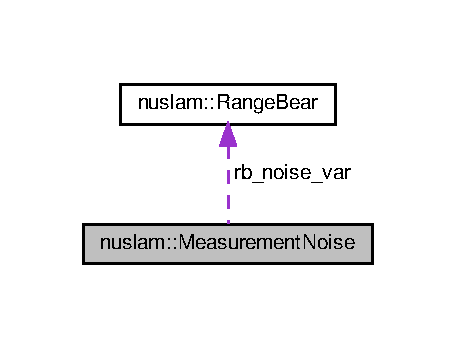
\includegraphics[width=219pt]{d8/de3/structnuslam_1_1MeasurementNoise__coll__graph}
\end{center}
\end{figure}
\subsection*{Public Member Functions}
\begin{DoxyCompactItemize}
\item 
\mbox{\Hypertarget{structnuslam_1_1MeasurementNoise_acad5ae4aedf60cfa75b7aa4432964010}\label{structnuslam_1_1MeasurementNoise_acad5ae4aedf60cfa75b7aa4432964010}} 
\hyperlink{structnuslam_1_1MeasurementNoise_acad5ae4aedf60cfa75b7aa4432964010}{Measurement\+Noise} ()
\begin{DoxyCompactList}\small\item\em constructor for Measurement noise matrix with xyt\+\_\+noise set to zero \end{DoxyCompactList}\item 
\mbox{\Hypertarget{structnuslam_1_1MeasurementNoise_abfbe4352cca0d9e8416142ce442f207e}\label{structnuslam_1_1MeasurementNoise_abfbe4352cca0d9e8416142ce442f207e}} 
\hyperlink{structnuslam_1_1MeasurementNoise_abfbe4352cca0d9e8416142ce442f207e}{Measurement\+Noise} (const \hyperlink{structnuslam_1_1RangeBear}{Range\+Bear} \&rb\+\_\+noise\+\_\+var\+\_\+)
\begin{DoxyCompactList}\small\item\em constructor for Measurement noise matrix with xyt\+\_\+noise set to user input \end{DoxyCompactList}\end{DoxyCompactItemize}
\subsection*{Public Attributes}
\begin{DoxyCompactItemize}
\item 
\mbox{\Hypertarget{structnuslam_1_1MeasurementNoise_a628b3f7c9c5a8a9aa53207d156ed7b0a}\label{structnuslam_1_1MeasurementNoise_a628b3f7c9c5a8a9aa53207d156ed7b0a}} 
\hyperlink{structnuslam_1_1RangeBear}{Range\+Bear} {\bfseries rb\+\_\+noise\+\_\+var}
\item 
\mbox{\Hypertarget{structnuslam_1_1MeasurementNoise_a857eb26ca831b2b4f4fe1d73e007a148}\label{structnuslam_1_1MeasurementNoise_a857eb26ca831b2b4f4fe1d73e007a148}} 
Eigen\+::\+Matrix\+Xd {\bfseries R}
\end{DoxyCompactItemize}


The documentation for this struct was generated from the following files\+:\begin{DoxyCompactItemize}
\item 
nuslam/include/nuslam/\hyperlink{ekf_8hpp}{ekf.\+hpp}\item 
nuslam/src/nuslam/ekf.\+cpp\end{DoxyCompactItemize}

\hypertarget{structnuslam_1_1Point}{}\section{nuslam\+:\+:Point Struct Reference}
\label{structnuslam_1_1Point}\index{nuslam\+::\+Point@{nuslam\+::\+Point}}


Collaboration diagram for nuslam\+:\+:Point\+:
\nopagebreak
\begin{figure}[H]
\begin{center}
\leavevmode
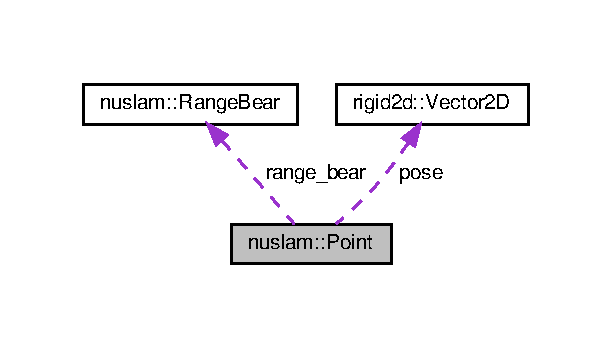
\includegraphics[width=294pt]{d4/d4a/structnuslam_1_1Point__coll__graph}
\end{center}
\end{figure}
\subsection*{Public Member Functions}
\begin{DoxyCompactItemize}
\item 
\mbox{\Hypertarget{structnuslam_1_1Point_a1cd12ede357a20cfbc3d640cea56a9ba}\label{structnuslam_1_1Point_a1cd12ede357a20cfbc3d640cea56a9ba}} 
{\bfseries Point} (const \hyperlink{structrigid2d_1_1Vector2D}{Vector2D} \&pose\+\_\+)
\item 
\mbox{\Hypertarget{structnuslam_1_1Point_ae021d2a3b0c1fc860170204937266e0b}\label{structnuslam_1_1Point_ae021d2a3b0c1fc860170204937266e0b}} 
{\bfseries Point} (const \hyperlink{structnuslam_1_1RangeBear}{Range\+Bear} \&range\+\_\+bear\+\_\+)
\end{DoxyCompactItemize}
\subsection*{Public Attributes}
\begin{DoxyCompactItemize}
\item 
\mbox{\Hypertarget{structnuslam_1_1Point_a9d15c2114308b18dc09d02ea937a49b4}\label{structnuslam_1_1Point_a9d15c2114308b18dc09d02ea937a49b4}} 
\hyperlink{structnuslam_1_1RangeBear}{Range\+Bear} {\bfseries range\+\_\+bear}
\item 
\mbox{\Hypertarget{structnuslam_1_1Point_ae1b635297f9325be42073330bb84e313}\label{structnuslam_1_1Point_ae1b635297f9325be42073330bb84e313}} 
\hyperlink{structrigid2d_1_1Vector2D}{Vector2D} {\bfseries pose}
\item 
\mbox{\Hypertarget{structnuslam_1_1Point_a11054da1181cccdae3641decfa504e42}\label{structnuslam_1_1Point_a11054da1181cccdae3641decfa504e42}} 
bool {\bfseries init}
\item 
\mbox{\Hypertarget{structnuslam_1_1Point_ac98cd6504662abd30438dd3c7d04c6f9}\label{structnuslam_1_1Point_ac98cd6504662abd30438dd3c7d04c6f9}} 
int {\bfseries index}
\item 
\mbox{\Hypertarget{structnuslam_1_1Point_a18c00024a973264ab5cad5c43fcd5bfc}\label{structnuslam_1_1Point_a18c00024a973264ab5cad5c43fcd5bfc}} 
int {\bfseries seen\+\_\+count}
\end{DoxyCompactItemize}


The documentation for this struct was generated from the following files\+:\begin{DoxyCompactItemize}
\item 
nuslam/include/nuslam/\hyperlink{landmarks_8hpp}{landmarks.\+hpp}\item 
nuslam/src/nuslam/landmarks.\+cpp\end{DoxyCompactItemize}

\hypertarget{structrigid2d_1_1Pose2D}{}\section{rigid2d\+:\+:Pose2D Struct Reference}
\label{structrigid2d_1_1Pose2D}\index{rigid2d\+::\+Pose2D@{rigid2d\+::\+Pose2D}}


A 2-\/\+Dimensional Pose.  




{\ttfamily \#include $<$diff\+\_\+drive.\+hpp$>$}

\subsection*{Public Member Functions}
\begin{DoxyCompactItemize}
\item 
\mbox{\Hypertarget{structrigid2d_1_1Pose2D_a03bb138e7b821c64241b8b6c2f633ec8}\label{structrigid2d_1_1Pose2D_a03bb138e7b821c64241b8b6c2f633ec8}} 
{\bfseries Pose2D} (double x\+\_\+, double y\+\_\+, double theta\+\_\+)
\end{DoxyCompactItemize}
\subsection*{Public Attributes}
\begin{DoxyCompactItemize}
\item 
\mbox{\Hypertarget{structrigid2d_1_1Pose2D_a706d15249c213d0236481ff1bd13c42d}\label{structrigid2d_1_1Pose2D_a706d15249c213d0236481ff1bd13c42d}} 
double {\bfseries x}
\item 
\mbox{\Hypertarget{structrigid2d_1_1Pose2D_a13f985853cc2b924ed87ed37e1857e7f}\label{structrigid2d_1_1Pose2D_a13f985853cc2b924ed87ed37e1857e7f}} 
double {\bfseries y}
\item 
\mbox{\Hypertarget{structrigid2d_1_1Pose2D_a4c872d777d0f72635b4c0c30c6d423c8}\label{structrigid2d_1_1Pose2D_a4c872d777d0f72635b4c0c30c6d423c8}} 
double {\bfseries theta}
\end{DoxyCompactItemize}


\subsection{Detailed Description}
A 2-\/\+Dimensional Pose. 

The documentation for this struct was generated from the following files\+:\begin{DoxyCompactItemize}
\item 
rigid2d/include/rigid2d/\hyperlink{diff__drive_8hpp}{diff\+\_\+drive.\+hpp}\item 
rigid2d/src/rigid2d/diff\+\_\+drive.\+cpp\end{DoxyCompactItemize}

\hypertarget{structnuslam_1_1ProcessNoise}{}\section{nuslam\+:\+:Process\+Noise Struct Reference}
\label{structnuslam_1_1ProcessNoise}\index{nuslam\+::\+Process\+Noise@{nuslam\+::\+Process\+Noise}}


Collaboration diagram for nuslam\+:\+:Process\+Noise\+:\nopagebreak
\begin{figure}[H]
\begin{center}
\leavevmode
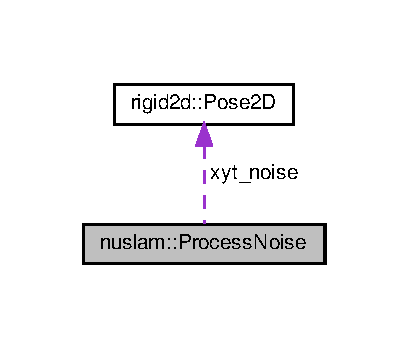
\includegraphics[width=196pt]{d7/d18/structnuslam_1_1ProcessNoise__coll__graph}
\end{center}
\end{figure}
\subsection*{Public Member Functions}
\begin{DoxyCompactItemize}
\item 
\mbox{\Hypertarget{structnuslam_1_1ProcessNoise_a9127539d5903305591394d3483d8b74b}\label{structnuslam_1_1ProcessNoise_a9127539d5903305591394d3483d8b74b}} 
\hyperlink{structnuslam_1_1ProcessNoise_a9127539d5903305591394d3483d8b74b}{Process\+Noise} ()
\begin{DoxyCompactList}\small\item\em constructor for process noise matrix with xyt\+\_\+noise set to zero \end{DoxyCompactList}\item 
\mbox{\Hypertarget{structnuslam_1_1ProcessNoise_accbf7987fa5b945ecae3a11d662ee6e7}\label{structnuslam_1_1ProcessNoise_accbf7987fa5b945ecae3a11d662ee6e7}} 
\hyperlink{structnuslam_1_1ProcessNoise_accbf7987fa5b945ecae3a11d662ee6e7}{Process\+Noise} (const \hyperlink{structrigid2d_1_1Pose2D}{Pose2D} \&xyt\+\_\+noise\+\_\+var, const unsigned long int \&map\+\_\+size\+\_\+)
\begin{DoxyCompactList}\small\item\em constructor for process noise matrix with xyt\+\_\+noise set to user input \end{DoxyCompactList}\end{DoxyCompactItemize}
\subsection*{Public Attributes}
\begin{DoxyCompactItemize}
\item 
\mbox{\Hypertarget{structnuslam_1_1ProcessNoise_a6f3cca68cb5cbea26a72324dde7787f2}\label{structnuslam_1_1ProcessNoise_a6f3cca68cb5cbea26a72324dde7787f2}} 
unsigned long int {\bfseries map\+\_\+size}
\item 
\mbox{\Hypertarget{structnuslam_1_1ProcessNoise_a1dc460a9ab6bb0e3f2c549c1cee87e42}\label{structnuslam_1_1ProcessNoise_a1dc460a9ab6bb0e3f2c549c1cee87e42}} 
\hyperlink{structrigid2d_1_1Pose2D}{Pose2D} {\bfseries xyt\+\_\+noise}
\item 
\mbox{\Hypertarget{structnuslam_1_1ProcessNoise_ab4c8c91544d776373fb415baf95cb9f8}\label{structnuslam_1_1ProcessNoise_ab4c8c91544d776373fb415baf95cb9f8}} 
Eigen\+::\+Matrix\+Xd {\bfseries q}
\item 
\mbox{\Hypertarget{structnuslam_1_1ProcessNoise_a01f5722b2393473f4bb3ccb2994a6dbe}\label{structnuslam_1_1ProcessNoise_a01f5722b2393473f4bb3ccb2994a6dbe}} 
Eigen\+::\+Matrix\+Xd {\bfseries Q}
\end{DoxyCompactItemize}


The documentation for this struct was generated from the following files\+:\begin{DoxyCompactItemize}
\item 
nuslam/include/nuslam/\hyperlink{ekf_8hpp}{ekf.\+hpp}\item 
nuslam/src/nuslam/ekf.\+cpp\end{DoxyCompactItemize}

\hypertarget{structnuslam_1_1RangeBear}{}\section{nuslam\+:\+:Range\+Bear Struct Reference}
\label{structnuslam_1_1RangeBear}\index{nuslam\+::\+Range\+Bear@{nuslam\+::\+Range\+Bear}}
\subsection*{Public Member Functions}
\begin{DoxyCompactItemize}
\item 
\mbox{\Hypertarget{structnuslam_1_1RangeBear_acafea61691e1944e68f033ff09d02ca0}\label{structnuslam_1_1RangeBear_acafea61691e1944e68f033ff09d02ca0}} 
{\bfseries Range\+Bear} (const double \&range\+\_\+, const double \&bearing\+\_\+)
\end{DoxyCompactItemize}
\subsection*{Public Attributes}
\begin{DoxyCompactItemize}
\item 
\mbox{\Hypertarget{structnuslam_1_1RangeBear_a1c6950401d08691b6cf6113bf3d35b25}\label{structnuslam_1_1RangeBear_a1c6950401d08691b6cf6113bf3d35b25}} 
double {\bfseries range}
\item 
\mbox{\Hypertarget{structnuslam_1_1RangeBear_a354541685ae24f2ed2e3503a7a96d5d6}\label{structnuslam_1_1RangeBear_a354541685ae24f2ed2e3503a7a96d5d6}} 
double {\bfseries bearing}
\end{DoxyCompactItemize}


The documentation for this struct was generated from the following files\+:\begin{DoxyCompactItemize}
\item 
nuslam/include/nuslam/\hyperlink{landmarks_8hpp}{landmarks.\+hpp}\item 
nuslam/src/nuslam/landmarks.\+cpp\end{DoxyCompactItemize}

\hypertarget{structrigid2d_1_1Screw2D}{}\section{rigid2d\+:\+:Screw2D Struct Reference}
\label{structrigid2d_1_1Screw2D}\index{rigid2d\+::\+Screw2D@{rigid2d\+::\+Screw2D}}


Screw Axis.  




{\ttfamily \#include $<$rigid2d.\+hpp$>$}

\subsection*{Public Member Functions}
\begin{DoxyCompactItemize}
\item 
\mbox{\Hypertarget{structrigid2d_1_1Screw2D_aafc846cdd1ce1482ac033720374a6581}\label{structrigid2d_1_1Screw2D_aafc846cdd1ce1482ac033720374a6581}} 
{\bfseries Screw2D} (double w\+\_\+z\+\_\+, double v\+\_\+x\+\_\+, double v\+\_\+y\+\_\+)
\end{DoxyCompactItemize}
\subsection*{Public Attributes}
\begin{DoxyCompactItemize}
\item 
\mbox{\Hypertarget{structrigid2d_1_1Screw2D_a834830a5bd4a0e86b51505405c10e6d7}\label{structrigid2d_1_1Screw2D_a834830a5bd4a0e86b51505405c10e6d7}} 
double {\bfseries w\+\_\+z}
\item 
\mbox{\Hypertarget{structrigid2d_1_1Screw2D_ac92d63f90c5cd05a8cbdbc8a30949596}\label{structrigid2d_1_1Screw2D_ac92d63f90c5cd05a8cbdbc8a30949596}} 
double {\bfseries v\+\_\+x}
\item 
\mbox{\Hypertarget{structrigid2d_1_1Screw2D_a8869a41619ecc359ff934d24189e85c7}\label{structrigid2d_1_1Screw2D_a8869a41619ecc359ff934d24189e85c7}} 
double {\bfseries v\+\_\+y}
\end{DoxyCompactItemize}


\subsection{Detailed Description}
Screw Axis. 

The documentation for this struct was generated from the following files\+:\begin{DoxyCompactItemize}
\item 
rigid2d/include/rigid2d/\hyperlink{rigid2d_8hpp}{rigid2d.\+hpp}\item 
rigid2d/src/rigid2d/rigid2d.\+cpp\end{DoxyCompactItemize}

\hypertarget{classrigid2d_1_1Transform2D}{}\section{rigid2d\+:\+:Transform2D Class Reference}
\label{classrigid2d_1_1Transform2D}\index{rigid2d\+::\+Transform2D@{rigid2d\+::\+Transform2D}}


a rigid body transformation in 2 dimensions  




{\ttfamily \#include $<$rigid2d.\+hpp$>$}

\subsection*{Public Member Functions}
\begin{DoxyCompactItemize}
\item 
\mbox{\Hypertarget{classrigid2d_1_1Transform2D_a455fbd07f86d3aeaaeca954a0904397a}\label{classrigid2d_1_1Transform2D_a455fbd07f86d3aeaaeca954a0904397a}} 
\hyperlink{classrigid2d_1_1Transform2D_a455fbd07f86d3aeaaeca954a0904397a}{Transform2D} ()
\begin{DoxyCompactList}\small\item\em Create an identity transformation. \end{DoxyCompactList}\item 
\hyperlink{classrigid2d_1_1Transform2D_ab3e595da2315ed50ba8eb24ead0c8d78}{Transform2D} (const \hyperlink{structrigid2d_1_1Vector2D}{Vector2D} \&trans)
\begin{DoxyCompactList}\small\item\em create a transformation that is a pure translation \end{DoxyCompactList}\item 
\hyperlink{classrigid2d_1_1Transform2D_a3f2f654cb039320e331931c0877b39a3}{Transform2D} (double radians)
\begin{DoxyCompactList}\small\item\em create a pure rotation \end{DoxyCompactList}\item 
\hyperlink{classrigid2d_1_1Transform2D_a47de6c24f25c57da553a0fdaf13e2138}{Transform2D} (const \hyperlink{structrigid2d_1_1Vector2D}{Vector2D} \&trans, double radians)
\begin{DoxyCompactList}\small\item\em Create a transformation with a translational and rotational component. \end{DoxyCompactList}\item 
\hyperlink{structrigid2d_1_1Vector2D}{Vector2D} \hyperlink{classrigid2d_1_1Transform2D_a80fbe5f0ea600b82812749d3c9e0f219}{operator()} (\hyperlink{structrigid2d_1_1Vector2D}{Vector2D} v) const
\begin{DoxyCompactList}\small\item\em apply a transformation to a \hyperlink{structrigid2d_1_1Vector2D}{Vector2D} \end{DoxyCompactList}\item 
\hyperlink{classrigid2d_1_1Transform2D}{Transform2D} \hyperlink{classrigid2d_1_1Transform2D_a2d324a150b852834b68629159e1b723b}{inv} () const
\begin{DoxyCompactList}\small\item\em invert the transformation \end{DoxyCompactList}\item 
\hyperlink{classrigid2d_1_1Transform2D}{Transform2D} \hyperlink{classrigid2d_1_1Transform2D_a56730e2d2c235e3909361cc0774f1c6e}{integrate\+Twist} (const \hyperlink{classrigid2d_1_1Twist2D}{Twist2D} \&tw) const
\begin{DoxyCompactList}\small\item\em compute transformation corresponding to a rigid body following a constant twist for one time unit \end{DoxyCompactList}\item 
\hyperlink{structrigid2d_1_1Transform2DS}{rigid2d\+::\+Transform2\+DS} \hyperlink{classrigid2d_1_1Transform2D_a2566972da0bb1c13f54b7ba948efd4f7}{displacement} () const
\begin{DoxyCompactList}\small\item\em return theta, x, y of Transform \end{DoxyCompactList}\item 
\hyperlink{classrigid2d_1_1Transform2D}{Transform2D} \& \hyperlink{classrigid2d_1_1Transform2D_a39a7a37c3be80717b8d2fe6cf00c1fbf}{operator$\ast$=} (const \hyperlink{classrigid2d_1_1Transform2D}{Transform2D} \&rhs)
\begin{DoxyCompactList}\small\item\em compose this transform with another and store the result in this object \end{DoxyCompactList}\end{DoxyCompactItemize}
\subsection*{Friends}
\begin{DoxyCompactItemize}
\item 
\mbox{\Hypertarget{classrigid2d_1_1Transform2D_addec8146e4e13196f026a35c51c03c55}\label{classrigid2d_1_1Transform2D_addec8146e4e13196f026a35c51c03c55}} 
class \hyperlink{classrigid2d_1_1Transform2D_addec8146e4e13196f026a35c51c03c55}{Twist2D}
\begin{DoxyCompactList}\small\item\em declare \hyperlink{classrigid2d_1_1Twist2D}{Twist2D} as friend so it can access \hyperlink{classrigid2d_1_1Transform2D}{Transform2D}\textquotesingle{}s private params \end{DoxyCompactList}\item 
\mbox{\Hypertarget{classrigid2d_1_1Transform2D_a43d7c8fc235f7592079bde4168cd48d8}\label{classrigid2d_1_1Transform2D_a43d7c8fc235f7592079bde4168cd48d8}} 
class \hyperlink{classrigid2d_1_1Transform2D_a43d7c8fc235f7592079bde4168cd48d8}{Diff\+Drive}
\begin{DoxyCompactList}\small\item\em declare \hyperlink{classrigid2d_1_1DiffDrive}{Diff\+Drive} as friend so it can access \hyperlink{classrigid2d_1_1Transform2D}{Transform2D}\textquotesingle{}s private params \end{DoxyCompactList}\item 
std\+::ostream \& \hyperlink{classrigid2d_1_1Transform2D_ad5239a3fa3a0f9cebd73c39f34c2075f}{operator$<$$<$} (std\+::ostream \&os, const \hyperlink{classrigid2d_1_1Transform2D}{Transform2D} \&tf)
\begin{DoxyCompactList}\small\item\em should print a human readable version of the transform\+: An example output\+: dtheta (degrees)\+: 90 dx\+: 3 dy\+: 5 \end{DoxyCompactList}\item 
std\+::istream \& \hyperlink{classrigid2d_1_1Transform2D_a7184f9b63deb3b10878054c34b02682b}{operator$>$$>$} (std\+::istream \&is, \hyperlink{classrigid2d_1_1Transform2D}{Transform2D} \&tf)
\begin{DoxyCompactList}\small\item\em Read a transformation from stdin Should be able to read input either as output by operator$<$$<$ or as 3 numbers (degrees, dx, dy) separated by spaces or newlines. \end{DoxyCompactList}\end{DoxyCompactItemize}


\subsection{Detailed Description}
a rigid body transformation in 2 dimensions 

\subsection{Constructor \& Destructor Documentation}
\mbox{\Hypertarget{classrigid2d_1_1Transform2D_ab3e595da2315ed50ba8eb24ead0c8d78}\label{classrigid2d_1_1Transform2D_ab3e595da2315ed50ba8eb24ead0c8d78}} 
\index{rigid2d\+::\+Transform2D@{rigid2d\+::\+Transform2D}!Transform2D@{Transform2D}}
\index{Transform2D@{Transform2D}!rigid2d\+::\+Transform2D@{rigid2d\+::\+Transform2D}}
\subsubsection{\texorpdfstring{Transform2\+D()}{Transform2D()}\hspace{0.1cm}{\footnotesize\ttfamily [1/3]}}
{\footnotesize\ttfamily rigid2d\+::\+Transform2\+D\+::\+Transform2D (\begin{DoxyParamCaption}\item[{const \hyperlink{structrigid2d_1_1Vector2D}{Vector2D} \&}]{trans }\end{DoxyParamCaption})\hspace{0.3cm}{\ttfamily [explicit]}}



create a transformation that is a pure translation 


\begin{DoxyParams}{Parameters}
{\em trans} & -\/ the vector by which to translate \\
\hline
\end{DoxyParams}
\mbox{\Hypertarget{classrigid2d_1_1Transform2D_a3f2f654cb039320e331931c0877b39a3}\label{classrigid2d_1_1Transform2D_a3f2f654cb039320e331931c0877b39a3}} 
\index{rigid2d\+::\+Transform2D@{rigid2d\+::\+Transform2D}!Transform2D@{Transform2D}}
\index{Transform2D@{Transform2D}!rigid2d\+::\+Transform2D@{rigid2d\+::\+Transform2D}}
\subsubsection{\texorpdfstring{Transform2\+D()}{Transform2D()}\hspace{0.1cm}{\footnotesize\ttfamily [2/3]}}
{\footnotesize\ttfamily rigid2d\+::\+Transform2\+D\+::\+Transform2D (\begin{DoxyParamCaption}\item[{double}]{radians }\end{DoxyParamCaption})\hspace{0.3cm}{\ttfamily [explicit]}}



create a pure rotation 


\begin{DoxyParams}{Parameters}
{\em radians} & -\/ angle of the rotation, in radians \\
\hline
\end{DoxyParams}
\mbox{\Hypertarget{classrigid2d_1_1Transform2D_a47de6c24f25c57da553a0fdaf13e2138}\label{classrigid2d_1_1Transform2D_a47de6c24f25c57da553a0fdaf13e2138}} 
\index{rigid2d\+::\+Transform2D@{rigid2d\+::\+Transform2D}!Transform2D@{Transform2D}}
\index{Transform2D@{Transform2D}!rigid2d\+::\+Transform2D@{rigid2d\+::\+Transform2D}}
\subsubsection{\texorpdfstring{Transform2\+D()}{Transform2D()}\hspace{0.1cm}{\footnotesize\ttfamily [3/3]}}
{\footnotesize\ttfamily rigid2d\+::\+Transform2\+D\+::\+Transform2D (\begin{DoxyParamCaption}\item[{const \hyperlink{structrigid2d_1_1Vector2D}{Vector2D} \&}]{trans,  }\item[{double}]{radians }\end{DoxyParamCaption})}



Create a transformation with a translational and rotational component. 


\begin{DoxyParams}{Parameters}
{\em trans} & -\/ the translation \\
\hline
{\em rot} & -\/ the rotation, in radians \\
\hline
\end{DoxyParams}


\subsection{Member Function Documentation}
\mbox{\Hypertarget{classrigid2d_1_1Transform2D_a2566972da0bb1c13f54b7ba948efd4f7}\label{classrigid2d_1_1Transform2D_a2566972da0bb1c13f54b7ba948efd4f7}} 
\index{rigid2d\+::\+Transform2D@{rigid2d\+::\+Transform2D}!displacement@{displacement}}
\index{displacement@{displacement}!rigid2d\+::\+Transform2D@{rigid2d\+::\+Transform2D}}
\subsubsection{\texorpdfstring{displacement()}{displacement()}}
{\footnotesize\ttfamily \hyperlink{structrigid2d_1_1Transform2DS}{rigid2d\+::\+Transform2\+DS} rigid2d\+::\+Transform2\+D\+::displacement (\begin{DoxyParamCaption}{ }\end{DoxyParamCaption}) const}



return theta, x, y of Transform 

\begin{DoxyReturn}{Returns}
\hyperlink{structrigid2d_1_1Transform2DS}{Transform2\+DS} struct with theta, x, y values. 
\end{DoxyReturn}
\mbox{\Hypertarget{classrigid2d_1_1Transform2D_a56730e2d2c235e3909361cc0774f1c6e}\label{classrigid2d_1_1Transform2D_a56730e2d2c235e3909361cc0774f1c6e}} 
\index{rigid2d\+::\+Transform2D@{rigid2d\+::\+Transform2D}!integrate\+Twist@{integrate\+Twist}}
\index{integrate\+Twist@{integrate\+Twist}!rigid2d\+::\+Transform2D@{rigid2d\+::\+Transform2D}}
\subsubsection{\texorpdfstring{integrate\+Twist()}{integrateTwist()}}
{\footnotesize\ttfamily \hyperlink{classrigid2d_1_1Transform2D}{rigid2d\+::\+Transform2D} rigid2d\+::\+Transform2\+D\+::integrate\+Twist (\begin{DoxyParamCaption}\item[{const \hyperlink{classrigid2d_1_1Twist2D}{Twist2D} \&}]{tw }\end{DoxyParamCaption}) const}



compute transformation corresponding to a rigid body following a constant twist for one time unit 


\begin{DoxyParams}{Parameters}
{\em tw} & -\/ \hyperlink{classrigid2d_1_1Twist2D}{Twist2D} which the transform follows \\
\hline
\end{DoxyParams}
\begin{DoxyReturn}{Returns}
new transformation of a rigid body following a twist 
\end{DoxyReturn}
\mbox{\Hypertarget{classrigid2d_1_1Transform2D_a2d324a150b852834b68629159e1b723b}\label{classrigid2d_1_1Transform2D_a2d324a150b852834b68629159e1b723b}} 
\index{rigid2d\+::\+Transform2D@{rigid2d\+::\+Transform2D}!inv@{inv}}
\index{inv@{inv}!rigid2d\+::\+Transform2D@{rigid2d\+::\+Transform2D}}
\subsubsection{\texorpdfstring{inv()}{inv()}}
{\footnotesize\ttfamily \hyperlink{classrigid2d_1_1Transform2D}{rigid2d\+::\+Transform2D} rigid2d\+::\+Transform2\+D\+::inv (\begin{DoxyParamCaption}{ }\end{DoxyParamCaption}) const}



invert the transformation 

\begin{DoxyReturn}{Returns}
the inverse transformation 
\end{DoxyReturn}
\mbox{\Hypertarget{classrigid2d_1_1Transform2D_a80fbe5f0ea600b82812749d3c9e0f219}\label{classrigid2d_1_1Transform2D_a80fbe5f0ea600b82812749d3c9e0f219}} 
\index{rigid2d\+::\+Transform2D@{rigid2d\+::\+Transform2D}!operator()@{operator()}}
\index{operator()@{operator()}!rigid2d\+::\+Transform2D@{rigid2d\+::\+Transform2D}}
\subsubsection{\texorpdfstring{operator()()}{operator()()}}
{\footnotesize\ttfamily \hyperlink{structrigid2d_1_1Vector2D}{rigid2d\+::\+Vector2D} rigid2d\+::\+Transform2\+D\+::operator() (\begin{DoxyParamCaption}\item[{\hyperlink{structrigid2d_1_1Vector2D}{rigid2d\+::\+Vector2D}}]{v }\end{DoxyParamCaption}) const}



apply a transformation to a \hyperlink{structrigid2d_1_1Vector2D}{Vector2D} 


\begin{DoxyParams}{Parameters}
{\em v} & -\/ the vector to transform \\
\hline
\end{DoxyParams}
\begin{DoxyReturn}{Returns}
a vector in the new coordinate system 
\end{DoxyReturn}
\mbox{\Hypertarget{classrigid2d_1_1Transform2D_a39a7a37c3be80717b8d2fe6cf00c1fbf}\label{classrigid2d_1_1Transform2D_a39a7a37c3be80717b8d2fe6cf00c1fbf}} 
\index{rigid2d\+::\+Transform2D@{rigid2d\+::\+Transform2D}!operator$\ast$=@{operator$\ast$=}}
\index{operator$\ast$=@{operator$\ast$=}!rigid2d\+::\+Transform2D@{rigid2d\+::\+Transform2D}}
\subsubsection{\texorpdfstring{operator$\ast$=()}{operator*=()}}
{\footnotesize\ttfamily \hyperlink{classrigid2d_1_1Transform2D}{rigid2d\+::\+Transform2D} \& rigid2d\+::\+Transform2\+D\+::operator$\ast$= (\begin{DoxyParamCaption}\item[{const \hyperlink{classrigid2d_1_1Transform2D}{Transform2D} \&}]{rhs }\end{DoxyParamCaption})}



compose this transform with another and store the result in this object 


\begin{DoxyParams}{Parameters}
{\em rhs} & -\/ the first transform to apply \\
\hline
\end{DoxyParams}
\begin{DoxyReturn}{Returns}
a reference to the newly transformed operator 
\end{DoxyReturn}


\subsection{Friends And Related Function Documentation}
\mbox{\Hypertarget{classrigid2d_1_1Transform2D_ad5239a3fa3a0f9cebd73c39f34c2075f}\label{classrigid2d_1_1Transform2D_ad5239a3fa3a0f9cebd73c39f34c2075f}} 
\index{rigid2d\+::\+Transform2D@{rigid2d\+::\+Transform2D}!operator$<$$<$@{operator$<$$<$}}
\index{operator$<$$<$@{operator$<$$<$}!rigid2d\+::\+Transform2D@{rigid2d\+::\+Transform2D}}
\subsubsection{\texorpdfstring{operator$<$$<$}{operator<<}}
{\footnotesize\ttfamily std\+::ostream\& operator$<$$<$ (\begin{DoxyParamCaption}\item[{std\+::ostream \&}]{os,  }\item[{const \hyperlink{classrigid2d_1_1Transform2D}{Transform2D} \&}]{tf }\end{DoxyParamCaption})\hspace{0.3cm}{\ttfamily [friend]}}



should print a human readable version of the transform\+: An example output\+: dtheta (degrees)\+: 90 dx\+: 3 dy\+: 5 

\begin{DoxySeeAlso}{See also}
operator$<$$<$(...) (declared outside this class) for a description. friend tag allows non-\/member functions to access private params.
\end{DoxySeeAlso}

\begin{DoxyParams}{Parameters}
{\em os} & -\/ an output stream \\
\hline
{\em tf} & -\/ the transform to print \\
\hline
\end{DoxyParams}
\mbox{\Hypertarget{classrigid2d_1_1Transform2D_a7184f9b63deb3b10878054c34b02682b}\label{classrigid2d_1_1Transform2D_a7184f9b63deb3b10878054c34b02682b}} 
\index{rigid2d\+::\+Transform2D@{rigid2d\+::\+Transform2D}!operator$>$$>$@{operator$>$$>$}}
\index{operator$>$$>$@{operator$>$$>$}!rigid2d\+::\+Transform2D@{rigid2d\+::\+Transform2D}}
\subsubsection{\texorpdfstring{operator$>$$>$}{operator>>}}
{\footnotesize\ttfamily std\+::istream\& operator$>$$>$ (\begin{DoxyParamCaption}\item[{std\+::istream \&}]{is,  }\item[{\hyperlink{classrigid2d_1_1Transform2D}{Transform2D} \&}]{tf }\end{DoxyParamCaption})\hspace{0.3cm}{\ttfamily [friend]}}



Read a transformation from stdin Should be able to read input either as output by operator$<$$<$ or as 3 numbers (degrees, dx, dy) separated by spaces or newlines. 

\begin{DoxySeeAlso}{See also}
operator$>$$>$(...) (declared outside this class) for a description. friend tag allows non-\/member functions to access private params. 
\end{DoxySeeAlso}


The documentation for this class was generated from the following files\+:\begin{DoxyCompactItemize}
\item 
rigid2d/include/rigid2d/\hyperlink{rigid2d_8hpp}{rigid2d.\+hpp}\item 
rigid2d/src/rigid2d/rigid2d.\+cpp\end{DoxyCompactItemize}

\hypertarget{structrigid2d_1_1Transform2DS}{}\section{rigid2d\+:\+:Transform2\+DS Struct Reference}
\label{structrigid2d_1_1Transform2DS}\index{rigid2d\+::\+Transform2\+DS@{rigid2d\+::\+Transform2\+DS}}


Struct version of \hyperlink{classrigid2d_1_1Transform2D}{Transform2D} to return private params.  




{\ttfamily \#include $<$rigid2d.\+hpp$>$}

\subsection*{Public Member Functions}
\begin{DoxyCompactItemize}
\item 
\mbox{\Hypertarget{structrigid2d_1_1Transform2DS_ab566ee31ab671eb49db65a254c52dc7d}\label{structrigid2d_1_1Transform2DS_ab566ee31ab671eb49db65a254c52dc7d}} 
{\bfseries Transform2\+DS} (double theta\+\_\+, double x\+\_\+, double y\+\_\+)
\end{DoxyCompactItemize}
\subsection*{Public Attributes}
\begin{DoxyCompactItemize}
\item 
\mbox{\Hypertarget{structrigid2d_1_1Transform2DS_a44142569bdca7073ad89509db66e511b}\label{structrigid2d_1_1Transform2DS_a44142569bdca7073ad89509db66e511b}} 
double {\bfseries theta}
\item 
\mbox{\Hypertarget{structrigid2d_1_1Transform2DS_a9fe0aecd3f0061557ca29194495f85bf}\label{structrigid2d_1_1Transform2DS_a9fe0aecd3f0061557ca29194495f85bf}} 
double {\bfseries x}
\item 
\mbox{\Hypertarget{structrigid2d_1_1Transform2DS_a1a4d9456f6dbe8a11ef90e1f1b09be84}\label{structrigid2d_1_1Transform2DS_a1a4d9456f6dbe8a11ef90e1f1b09be84}} 
double {\bfseries y}
\end{DoxyCompactItemize}


\subsection{Detailed Description}
Struct version of \hyperlink{classrigid2d_1_1Transform2D}{Transform2D} to return private params. 

The documentation for this struct was generated from the following files\+:\begin{DoxyCompactItemize}
\item 
rigid2d/include/rigid2d/\hyperlink{rigid2d_8hpp}{rigid2d.\+hpp}\item 
rigid2d/src/rigid2d/rigid2d.\+cpp\end{DoxyCompactItemize}

\hypertarget{classgazebo_1_1TurtleDrivePlugin}{}\section{gazebo\+:\+:Turtle\+Drive\+Plugin Class Reference}
\label{classgazebo_1_1TurtleDrivePlugin}\index{gazebo\+::\+Turtle\+Drive\+Plugin@{gazebo\+::\+Turtle\+Drive\+Plugin}}


Inheritance diagram for gazebo\+:\+:Turtle\+Drive\+Plugin\+:
\nopagebreak
\begin{figure}[H]
\begin{center}
\leavevmode
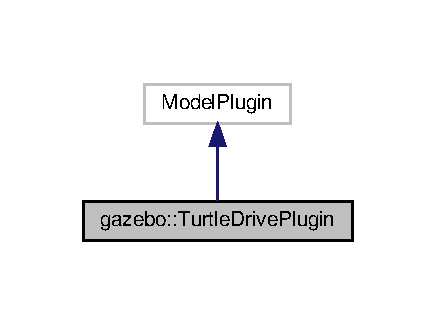
\includegraphics[width=209pt]{d6/d21/classgazebo_1_1TurtleDrivePlugin__inherit__graph}
\end{center}
\end{figure}


Collaboration diagram for gazebo\+:\+:Turtle\+Drive\+Plugin\+:
\nopagebreak
\begin{figure}[H]
\begin{center}
\leavevmode
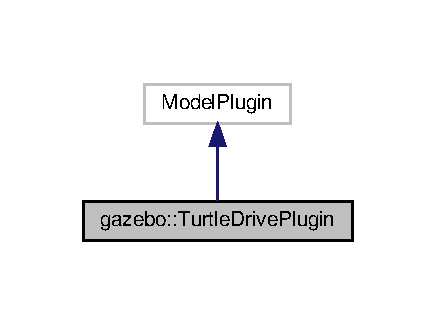
\includegraphics[width=209pt]{da/d2c/classgazebo_1_1TurtleDrivePlugin__coll__graph}
\end{center}
\end{figure}
\subsection*{Public Member Functions}
\begin{DoxyCompactItemize}
\item 
\hyperlink{classgazebo_1_1TurtleDrivePlugin_a7a36efc4658c4e4b1cedcdd70517e7dc}{Turtle\+Drive\+Plugin} ()
\begin{DoxyCompactList}\small\item\em Constructor for \hyperlink{classgazebo_1_1TurtleDrivePlugin}{Turtle\+Drive\+Plugin}. Models real Turtlebot interface for use in Gazebo. \end{DoxyCompactList}\item 
void \hyperlink{classgazebo_1_1TurtleDrivePlugin_ab80df6990ee5bc40d968834ba97c7bb2}{wheel\+\_\+cmd\+Callback} (const nuturtlebot\+::\+Wheel\+Commands \&wc)
\begin{DoxyCompactList}\small\item\em callback to convert wheel commands (+-\/ 256) to velocities and applies them to gazebo model \end{DoxyCompactList}\item 
virtual void \hyperlink{classgazebo_1_1TurtleDrivePlugin_a41993122444281e45f38a5e5171be76a}{Load} (physics\+::\+Model\+Ptr \+\_\+model, sdf\+::\+Element\+Ptr \+\_\+sdf)
\begin{DoxyCompactList}\small\item\em Loads the plugin and uses the physics\+::\+Model\+Ptr object to manipulate model physics and the sdf\+::\+Element\+Ptr to read user-\/specified parameters such as joint names and ros topics. \end{DoxyCompactList}\end{DoxyCompactItemize}


\subsection{Constructor \& Destructor Documentation}
\mbox{\Hypertarget{classgazebo_1_1TurtleDrivePlugin_a7a36efc4658c4e4b1cedcdd70517e7dc}\label{classgazebo_1_1TurtleDrivePlugin_a7a36efc4658c4e4b1cedcdd70517e7dc}} 
\index{gazebo\+::\+Turtle\+Drive\+Plugin@{gazebo\+::\+Turtle\+Drive\+Plugin}!Turtle\+Drive\+Plugin@{Turtle\+Drive\+Plugin}}
\index{Turtle\+Drive\+Plugin@{Turtle\+Drive\+Plugin}!gazebo\+::\+Turtle\+Drive\+Plugin@{gazebo\+::\+Turtle\+Drive\+Plugin}}
\subsubsection{\texorpdfstring{Turtle\+Drive\+Plugin()}{TurtleDrivePlugin()}}
{\footnotesize\ttfamily gazebo\+::\+Turtle\+Drive\+Plugin\+::\+Turtle\+Drive\+Plugin (\begin{DoxyParamCaption}{ }\end{DoxyParamCaption})}



Constructor for \hyperlink{classgazebo_1_1TurtleDrivePlugin}{Turtle\+Drive\+Plugin}. Models real Turtlebot interface for use in Gazebo. 

empty constructor for plugin 

\subsection{Member Function Documentation}
\mbox{\Hypertarget{classgazebo_1_1TurtleDrivePlugin_a41993122444281e45f38a5e5171be76a}\label{classgazebo_1_1TurtleDrivePlugin_a41993122444281e45f38a5e5171be76a}} 
\index{gazebo\+::\+Turtle\+Drive\+Plugin@{gazebo\+::\+Turtle\+Drive\+Plugin}!Load@{Load}}
\index{Load@{Load}!gazebo\+::\+Turtle\+Drive\+Plugin@{gazebo\+::\+Turtle\+Drive\+Plugin}}
\subsubsection{\texorpdfstring{Load()}{Load()}}
{\footnotesize\ttfamily void gazebo\+::\+Turtle\+Drive\+Plugin\+::\+Load (\begin{DoxyParamCaption}\item[{physics\+::\+Model\+Ptr}]{\+\_\+model,  }\item[{sdf\+::\+Element\+Ptr}]{\+\_\+sdf }\end{DoxyParamCaption})\hspace{0.3cm}{\ttfamily [virtual]}}



Loads the plugin and uses the physics\+::\+Model\+Ptr object to manipulate model physics and the sdf\+::\+Element\+Ptr to read user-\/specified parameters such as joint names and ros topics. 


\begin{DoxyParams}{Parameters}
{\em physics\+::\+Model\+Ptr} & pointer to manipulate model physics (set joint speeds/torques etc) \\
\hline
{\em sdf\+::\+Element\+Ptr} & pointer to read user input from .gazebo.\+xacro file to set plugin parameters \\
\hline
\end{DoxyParams}
\mbox{\Hypertarget{classgazebo_1_1TurtleDrivePlugin_ab80df6990ee5bc40d968834ba97c7bb2}\label{classgazebo_1_1TurtleDrivePlugin_ab80df6990ee5bc40d968834ba97c7bb2}} 
\index{gazebo\+::\+Turtle\+Drive\+Plugin@{gazebo\+::\+Turtle\+Drive\+Plugin}!wheel\+\_\+cmd\+Callback@{wheel\+\_\+cmd\+Callback}}
\index{wheel\+\_\+cmd\+Callback@{wheel\+\_\+cmd\+Callback}!gazebo\+::\+Turtle\+Drive\+Plugin@{gazebo\+::\+Turtle\+Drive\+Plugin}}
\subsubsection{\texorpdfstring{wheel\+\_\+cmd\+Callback()}{wheel\_cmdCallback()}}
{\footnotesize\ttfamily void gazebo\+::\+Turtle\+Drive\+Plugin\+::wheel\+\_\+cmd\+Callback (\begin{DoxyParamCaption}\item[{const nuturtlebot\+::\+Wheel\+Commands \&}]{wc }\end{DoxyParamCaption})}



callback to convert wheel commands (+-\/ 256) to velocities and applies them to gazebo model 


\begin{DoxyParams}{Parameters}
{\em nuturtlebot\+::\+Wheel\+Commands} & integer value between +-\/256 to indicate wheel speed \\
\hline
\end{DoxyParams}


The documentation for this class was generated from the following files\+:\begin{DoxyCompactItemize}
\item 
nuturtle\+\_\+gazebo/include/nuturtle\+\_\+gazebo/turtle\+\_\+drive\+\_\+plugin.\+hpp\item 
nuturtle\+\_\+gazebo/src/turtle\+\_\+drive\+\_\+plugin.\+cpp\end{DoxyCompactItemize}

\hypertarget{classrigid2d_1_1Twist2D}{}\section{rigid2d\+:\+:Twist2D Class Reference}
\label{classrigid2d_1_1Twist2D}\index{rigid2d\+::\+Twist2D@{rigid2d\+::\+Twist2D}}


a two-\/dimensional twist  




{\ttfamily \#include $<$rigid2d.\+hpp$>$}

\subsection*{Public Member Functions}
\begin{DoxyCompactItemize}
\item 
\mbox{\Hypertarget{classrigid2d_1_1Twist2D_a8a317315c9dc111b01e0f3c53af072b4}\label{classrigid2d_1_1Twist2D_a8a317315c9dc111b01e0f3c53af072b4}} 
\hyperlink{classrigid2d_1_1Twist2D_a8a317315c9dc111b01e0f3c53af072b4}{Twist2D} ()
\begin{DoxyCompactList}\small\item\em Create a zero-\/\+Twist. \end{DoxyCompactList}\item 
\mbox{\Hypertarget{classrigid2d_1_1Twist2D_ac08464a283d6577dd5daffb82b2652ce}\label{classrigid2d_1_1Twist2D_ac08464a283d6577dd5daffb82b2652ce}} 
\hyperlink{classrigid2d_1_1Twist2D_ac08464a283d6577dd5daffb82b2652ce}{Twist2D} (double w\+\_\+z\+\_\+, double v\+\_\+x\+\_\+, double v\+\_\+y\+\_\+)
\begin{DoxyCompactList}\small\item\em Create a non-\/zero Twist. \end{DoxyCompactList}\item 
\hyperlink{classrigid2d_1_1Twist2D}{Twist2D} \hyperlink{classrigid2d_1_1Twist2D_af5d38e8a9b62c7f414453ea37e012697}{convert} (const \hyperlink{classrigid2d_1_1Transform2D}{Transform2D} \&tf) const
\begin{DoxyCompactList}\small\item\em convert the twist using an adjoint \end{DoxyCompactList}\item 
\mbox{\Hypertarget{classrigid2d_1_1Twist2D_af9c23f13a251cbb56210a9fa870102ea}\label{classrigid2d_1_1Twist2D_af9c23f13a251cbb56210a9fa870102ea}} 
void \hyperlink{classrigid2d_1_1Twist2D_af9c23f13a251cbb56210a9fa870102ea}{reassign} (double w\+\_\+z\+\_\+, double v\+\_\+x\+\_\+, double v\+\_\+y\+\_\+)
\begin{DoxyCompactList}\small\item\em reassign \hyperlink{classrigid2d_1_1Twist2D}{Twist2D} values \end{DoxyCompactList}\end{DoxyCompactItemize}
\subsection*{Public Attributes}
\begin{DoxyCompactItemize}
\item 
\mbox{\Hypertarget{classrigid2d_1_1Twist2D_ad2f8bedd3dab17667975cac0b2742d45}\label{classrigid2d_1_1Twist2D_ad2f8bedd3dab17667975cac0b2742d45}} 
double {\bfseries v\+\_\+x}
\item 
\mbox{\Hypertarget{classrigid2d_1_1Twist2D_a3daf139ba86cb48702e00ac5a815a56c}\label{classrigid2d_1_1Twist2D_a3daf139ba86cb48702e00ac5a815a56c}} 
double {\bfseries v\+\_\+y}
\item 
\mbox{\Hypertarget{classrigid2d_1_1Twist2D_aa1c51383a57fe07b3a944f99801d2058}\label{classrigid2d_1_1Twist2D_aa1c51383a57fe07b3a944f99801d2058}} 
double {\bfseries w\+\_\+z}
\end{DoxyCompactItemize}
\subsection*{Friends}
\begin{DoxyCompactItemize}
\item 
\mbox{\Hypertarget{classrigid2d_1_1Twist2D_a49f4e819b5084b5347aff6e6559b596b}\label{classrigid2d_1_1Twist2D_a49f4e819b5084b5347aff6e6559b596b}} 
class \hyperlink{classrigid2d_1_1Twist2D_a49f4e819b5084b5347aff6e6559b596b}{Transform2D}
\begin{DoxyCompactList}\small\item\em declare \hyperlink{classrigid2d_1_1Transform2D}{Transform2D} as friend so it can access \hyperlink{classrigid2d_1_1Twist2D}{Twist2D}\textquotesingle{}s private params \end{DoxyCompactList}\item 
\mbox{\Hypertarget{classrigid2d_1_1Twist2D_a43d7c8fc235f7592079bde4168cd48d8}\label{classrigid2d_1_1Twist2D_a43d7c8fc235f7592079bde4168cd48d8}} 
class {\bfseries Diff\+Drive}
\item 
\mbox{\Hypertarget{classrigid2d_1_1Twist2D_afeca09cf85f3491b24cdc9f9d41bab3d}\label{classrigid2d_1_1Twist2D_afeca09cf85f3491b24cdc9f9d41bab3d}} 
class {\bfseries Waypoints}
\item 
std\+::ostream \& \hyperlink{classrigid2d_1_1Twist2D_aa73bc548f9e2f87b66c08cd96443e792}{operator$<$$<$} (std\+::ostream \&os, const \hyperlink{classrigid2d_1_1Twist2D}{Twist2D} \&tw)
\begin{DoxyCompactList}\small\item\em should print a human readable version of the twist\+: An example output\+: dtheta (degrees)\+: 90 dx\+: 3 dy\+: 5 \end{DoxyCompactList}\item 
std\+::istream \& \hyperlink{classrigid2d_1_1Twist2D_a123979c39440643723bcd0e3e04812df}{operator$>$$>$} (std\+::istream \&is, \hyperlink{classrigid2d_1_1Twist2D}{Twist2D} \&tw)
\begin{DoxyCompactList}\small\item\em Read a twist from stdin Should be able to read input either as output by operator$<$$<$ or as 3 numbers (w\+\_\+z, v\+\_\+x, v\+\_\+y) separated by spaces or newlines. \end{DoxyCompactList}\end{DoxyCompactItemize}


\subsection{Detailed Description}
a two-\/dimensional twist 

\subsection{Member Function Documentation}
\mbox{\Hypertarget{classrigid2d_1_1Twist2D_af5d38e8a9b62c7f414453ea37e012697}\label{classrigid2d_1_1Twist2D_af5d38e8a9b62c7f414453ea37e012697}} 
\index{rigid2d\+::\+Twist2D@{rigid2d\+::\+Twist2D}!convert@{convert}}
\index{convert@{convert}!rigid2d\+::\+Twist2D@{rigid2d\+::\+Twist2D}}
\subsubsection{\texorpdfstring{convert()}{convert()}}
{\footnotesize\ttfamily \hyperlink{classrigid2d_1_1Twist2D}{rigid2d\+::\+Twist2D} rigid2d\+::\+Twist2\+D\+::convert (\begin{DoxyParamCaption}\item[{const \hyperlink{classrigid2d_1_1Transform2D}{Transform2D} \&}]{tf }\end{DoxyParamCaption}) const}



convert the twist using an adjoint 


\begin{DoxyParams}{Parameters}
{\em tf} & -\/ the frame to which the twist is converted. \\
\hline
\end{DoxyParams}
\begin{DoxyReturn}{Returns}
the converted twist. 
\end{DoxyReturn}


\subsection{Friends And Related Function Documentation}
\mbox{\Hypertarget{classrigid2d_1_1Twist2D_aa73bc548f9e2f87b66c08cd96443e792}\label{classrigid2d_1_1Twist2D_aa73bc548f9e2f87b66c08cd96443e792}} 
\index{rigid2d\+::\+Twist2D@{rigid2d\+::\+Twist2D}!operator$<$$<$@{operator$<$$<$}}
\index{operator$<$$<$@{operator$<$$<$}!rigid2d\+::\+Twist2D@{rigid2d\+::\+Twist2D}}
\subsubsection{\texorpdfstring{operator$<$$<$}{operator<<}}
{\footnotesize\ttfamily std\+::ostream\& operator$<$$<$ (\begin{DoxyParamCaption}\item[{std\+::ostream \&}]{os,  }\item[{const \hyperlink{classrigid2d_1_1Twist2D}{Twist2D} \&}]{tw }\end{DoxyParamCaption})\hspace{0.3cm}{\ttfamily [friend]}}



should print a human readable version of the twist\+: An example output\+: dtheta (degrees)\+: 90 dx\+: 3 dy\+: 5 

\begin{DoxySeeAlso}{See also}
operator$<$$<$(...) (declared outside this class) for a description. friend tag allows non-\/member functions to access private params.
\end{DoxySeeAlso}

\begin{DoxyParams}{Parameters}
{\em os} & -\/ an output stream \\
\hline
{\em tf} & -\/ the twist to print \\
\hline
\end{DoxyParams}
\mbox{\Hypertarget{classrigid2d_1_1Twist2D_a123979c39440643723bcd0e3e04812df}\label{classrigid2d_1_1Twist2D_a123979c39440643723bcd0e3e04812df}} 
\index{rigid2d\+::\+Twist2D@{rigid2d\+::\+Twist2D}!operator$>$$>$@{operator$>$$>$}}
\index{operator$>$$>$@{operator$>$$>$}!rigid2d\+::\+Twist2D@{rigid2d\+::\+Twist2D}}
\subsubsection{\texorpdfstring{operator$>$$>$}{operator>>}}
{\footnotesize\ttfamily std\+::istream\& operator$>$$>$ (\begin{DoxyParamCaption}\item[{std\+::istream \&}]{is,  }\item[{\hyperlink{classrigid2d_1_1Twist2D}{Twist2D} \&}]{tw }\end{DoxyParamCaption})\hspace{0.3cm}{\ttfamily [friend]}}



Read a twist from stdin Should be able to read input either as output by operator$<$$<$ or as 3 numbers (w\+\_\+z, v\+\_\+x, v\+\_\+y) separated by spaces or newlines. 

\begin{DoxySeeAlso}{See also}
operator$>$$>$(...) (declared outside this class) for a description. friend tag allows non-\/member functions to access private params. 
\end{DoxySeeAlso}


The documentation for this class was generated from the following files\+:\begin{DoxyCompactItemize}
\item 
rigid2d/include/rigid2d/\hyperlink{rigid2d_8hpp}{rigid2d.\+hpp}\item 
rigid2d/src/rigid2d/rigid2d.\+cpp\end{DoxyCompactItemize}

\hypertarget{structrigid2d_1_1Vector2D}{}\section{rigid2d\+:\+:Vector2D Struct Reference}
\label{structrigid2d_1_1Vector2D}\index{rigid2d\+::\+Vector2D@{rigid2d\+::\+Vector2D}}


A 2-\/\+Dimensional Vector.  




{\ttfamily \#include $<$rigid2d.\+hpp$>$}

\subsection*{Public Member Functions}
\begin{DoxyCompactItemize}
\item 
\mbox{\Hypertarget{structrigid2d_1_1Vector2D_a7676be61234533fc4c569fc27fd78a9e}\label{structrigid2d_1_1Vector2D_a7676be61234533fc4c569fc27fd78a9e}} 
{\bfseries Vector2D} (double x\+\_\+, double y\+\_\+)
\item 
\mbox{\Hypertarget{structrigid2d_1_1Vector2D_a0be56967b3920a398291ea722c540114}\label{structrigid2d_1_1Vector2D_a0be56967b3920a398291ea722c540114}} 
void {\bfseries normalize} ()
\item 
\hyperlink{structrigid2d_1_1Vector2D}{Vector2D} \& \hyperlink{structrigid2d_1_1Vector2D_a2e20ab3a7d186527955370e58df504ec}{operator+=} (const \hyperlink{structrigid2d_1_1Vector2D}{Vector2D} \&rhs)
\begin{DoxyCompactList}\small\item\em perform vector addition \end{DoxyCompactList}\item 
\hyperlink{structrigid2d_1_1Vector2D}{Vector2D} \& \hyperlink{structrigid2d_1_1Vector2D_a43ee2a20c766c24809e243cebbdae224}{operator-\/=} (const \hyperlink{structrigid2d_1_1Vector2D}{Vector2D} \&rhs)
\begin{DoxyCompactList}\small\item\em perform vector subtraction \end{DoxyCompactList}\item 
\hyperlink{structrigid2d_1_1Vector2D}{Vector2D} \& \hyperlink{structrigid2d_1_1Vector2D_a28ed19c24dd07b32695109c55fe95686}{operator$\ast$=} (const double \&scalar)
\begin{DoxyCompactList}\small\item\em perform scalar multiplication on a vector \end{DoxyCompactList}\end{DoxyCompactItemize}
\subsection*{Public Attributes}
\begin{DoxyCompactItemize}
\item 
\mbox{\Hypertarget{structrigid2d_1_1Vector2D_a1876d655fe2da548c4813777c450845c}\label{structrigid2d_1_1Vector2D_a1876d655fe2da548c4813777c450845c}} 
double {\bfseries x}
\item 
\mbox{\Hypertarget{structrigid2d_1_1Vector2D_aa814ea37ffe4a161b0020609580e4d17}\label{structrigid2d_1_1Vector2D_aa814ea37ffe4a161b0020609580e4d17}} 
double {\bfseries y}
\item 
\mbox{\Hypertarget{structrigid2d_1_1Vector2D_a187215ccee09402486afad8107592639}\label{structrigid2d_1_1Vector2D_a187215ccee09402486afad8107592639}} 
double {\bfseries norm\+\_\+x}
\item 
\mbox{\Hypertarget{structrigid2d_1_1Vector2D_ad4a3b1bc820490672c5a339e61ff8db2}\label{structrigid2d_1_1Vector2D_ad4a3b1bc820490672c5a339e61ff8db2}} 
double {\bfseries norm\+\_\+y}
\end{DoxyCompactItemize}


\subsection{Detailed Description}
A 2-\/\+Dimensional Vector. 

static\+\_\+assertions test compile time assumptions. You should write at least one more test for each function You should also purposely (and temporarily) make one of these tests fail just to see what happens 

\subsection{Member Function Documentation}
\mbox{\Hypertarget{structrigid2d_1_1Vector2D_a28ed19c24dd07b32695109c55fe95686}\label{structrigid2d_1_1Vector2D_a28ed19c24dd07b32695109c55fe95686}} 
\index{rigid2d\+::\+Vector2D@{rigid2d\+::\+Vector2D}!operator$\ast$=@{operator$\ast$=}}
\index{operator$\ast$=@{operator$\ast$=}!rigid2d\+::\+Vector2D@{rigid2d\+::\+Vector2D}}
\subsubsection{\texorpdfstring{operator$\ast$=()}{operator*=()}}
{\footnotesize\ttfamily \hyperlink{structrigid2d_1_1Vector2D}{rigid2d\+::\+Vector2D} \& rigid2d\+::\+Vector2\+D\+::operator$\ast$= (\begin{DoxyParamCaption}\item[{const double \&}]{scalar }\end{DoxyParamCaption})}



perform scalar multiplication on a vector 


\begin{DoxyParams}{Parameters}
{\em rhs} & -\/ the vector to add \\
\hline
\end{DoxyParams}
\begin{DoxyReturn}{Returns}
a reference to the newly transformed operator 
\end{DoxyReturn}
\mbox{\Hypertarget{structrigid2d_1_1Vector2D_a2e20ab3a7d186527955370e58df504ec}\label{structrigid2d_1_1Vector2D_a2e20ab3a7d186527955370e58df504ec}} 
\index{rigid2d\+::\+Vector2D@{rigid2d\+::\+Vector2D}!operator+=@{operator+=}}
\index{operator+=@{operator+=}!rigid2d\+::\+Vector2D@{rigid2d\+::\+Vector2D}}
\subsubsection{\texorpdfstring{operator+=()}{operator+=()}}
{\footnotesize\ttfamily \hyperlink{structrigid2d_1_1Vector2D}{rigid2d\+::\+Vector2D} \& rigid2d\+::\+Vector2\+D\+::operator+= (\begin{DoxyParamCaption}\item[{const \hyperlink{structrigid2d_1_1Vector2D}{Vector2D} \&}]{rhs }\end{DoxyParamCaption})}



perform vector addition 


\begin{DoxyParams}{Parameters}
{\em rhs} & -\/ the vector to add \\
\hline
\end{DoxyParams}
\begin{DoxyReturn}{Returns}
a reference to the newly transformed operator 
\end{DoxyReturn}
\mbox{\Hypertarget{structrigid2d_1_1Vector2D_a43ee2a20c766c24809e243cebbdae224}\label{structrigid2d_1_1Vector2D_a43ee2a20c766c24809e243cebbdae224}} 
\index{rigid2d\+::\+Vector2D@{rigid2d\+::\+Vector2D}!operator-\/=@{operator-\/=}}
\index{operator-\/=@{operator-\/=}!rigid2d\+::\+Vector2D@{rigid2d\+::\+Vector2D}}
\subsubsection{\texorpdfstring{operator-\/=()}{operator-=()}}
{\footnotesize\ttfamily \hyperlink{structrigid2d_1_1Vector2D}{rigid2d\+::\+Vector2D} \& rigid2d\+::\+Vector2\+D\+::operator-\/= (\begin{DoxyParamCaption}\item[{const \hyperlink{structrigid2d_1_1Vector2D}{Vector2D} \&}]{rhs }\end{DoxyParamCaption})}



perform vector subtraction 


\begin{DoxyParams}{Parameters}
{\em rhs} & -\/ the vector to subtract \\
\hline
\end{DoxyParams}
\begin{DoxyReturn}{Returns}
a reference to the newly transformed operator 
\end{DoxyReturn}


The documentation for this struct was generated from the following files\+:\begin{DoxyCompactItemize}
\item 
rigid2d/include/rigid2d/\hyperlink{rigid2d_8hpp}{rigid2d.\+hpp}\item 
rigid2d/src/rigid2d/rigid2d.\+cpp\end{DoxyCompactItemize}

\hypertarget{classrigid2d_1_1Waypoints}{}\section{rigid2d\+:\+:Waypoints Class Reference}
\label{classrigid2d_1_1Waypoints}\index{rigid2d\+::\+Waypoints@{rigid2d\+::\+Waypoints}}
\subsection*{Public Member Functions}
\begin{DoxyCompactItemize}
\item 
\mbox{\Hypertarget{classrigid2d_1_1Waypoints_a8e7579d65c588966c0f53866a73fee43}\label{classrigid2d_1_1Waypoints_a8e7579d65c588966c0f53866a73fee43}} 
\hyperlink{classrigid2d_1_1Waypoints_a8e7579d65c588966c0f53866a73fee43}{Waypoints} ()
\begin{DoxyCompactList}\small\item\em the default constructor creates a vectour of four waypoints in a rectangle \end{DoxyCompactList}\item 
\hyperlink{classrigid2d_1_1Waypoints_a2d80cabdd52bc5291ddab198be441618}{Waypoints} (const std\+::vector$<$ \hyperlink{structrigid2d_1_1Vector2D}{Vector2D} $>$ \&waypoints\+\_\+)
\begin{DoxyCompactList}\small\item\em create a \hyperlink{classrigid2d_1_1Waypoints}{Waypoints} instance by specifying the waypoints to visit in a vector \end{DoxyCompactList}\item 
\hyperlink{classrigid2d_1_1Waypoints_a45bc2c3d9687047b403d08f14456961e}{Waypoints} (const std\+::vector$<$ \hyperlink{structrigid2d_1_1Vector2D}{Vector2D} $>$ \&waypoints\+\_\+, const double \&P\+\_\+h\+\_\+, const double \&P\+\_\+l\+\_\+, const double \&w\+\_\+z\+\_\+max\+\_\+, const double \&v\+\_\+x\+\_\+max\+\_\+, const double \&threshold\+\_\+)
\begin{DoxyCompactList}\small\item\em create a \hyperlink{classrigid2d_1_1Waypoints}{Waypoints} instance by specifying the waypoints to visit in a vector, the proportional controller gains, the maximum twist thresholds and the pose threshold \end{DoxyCompactList}\item 
\hyperlink{classrigid2d_1_1Twist2D}{Twist2D} \hyperlink{classrigid2d_1_1Waypoints_a9431a48c1fad67270b4fe27712fee09a}{next\+Waypoint} (const \hyperlink{structrigid2d_1_1Pose2D}{Pose2D} \&pose)
\begin{DoxyCompactList}\small\item\em computes the required \hyperlink{classrigid2d_1_1Twist2D}{Twist2D} to reach the next waypoint, whether linear or angular, and pushes waypoints back for cyclical motion when necessary \end{DoxyCompactList}\end{DoxyCompactItemize}


\subsection{Constructor \& Destructor Documentation}
\mbox{\Hypertarget{classrigid2d_1_1Waypoints_a2d80cabdd52bc5291ddab198be441618}\label{classrigid2d_1_1Waypoints_a2d80cabdd52bc5291ddab198be441618}} 
\index{rigid2d\+::\+Waypoints@{rigid2d\+::\+Waypoints}!Waypoints@{Waypoints}}
\index{Waypoints@{Waypoints}!rigid2d\+::\+Waypoints@{rigid2d\+::\+Waypoints}}
\subsubsection{\texorpdfstring{Waypoints()}{Waypoints()}\hspace{0.1cm}{\footnotesize\ttfamily [1/2]}}
{\footnotesize\ttfamily rigid2d\+::\+Waypoints\+::\+Waypoints (\begin{DoxyParamCaption}\item[{const std\+::vector$<$ \hyperlink{structrigid2d_1_1Vector2D}{Vector2D} $>$ \&}]{waypoints\+\_\+ }\end{DoxyParamCaption})}



create a \hyperlink{classrigid2d_1_1Waypoints}{Waypoints} instance by specifying the waypoints to visit in a vector 


\begin{DoxyParams}{Parameters}
{\em std\+::vector$<$rigid2d\+::\+Vector2\+D$>$} & -\/ the waypoints to visit \\
\hline
\end{DoxyParams}
\mbox{\Hypertarget{classrigid2d_1_1Waypoints_a45bc2c3d9687047b403d08f14456961e}\label{classrigid2d_1_1Waypoints_a45bc2c3d9687047b403d08f14456961e}} 
\index{rigid2d\+::\+Waypoints@{rigid2d\+::\+Waypoints}!Waypoints@{Waypoints}}
\index{Waypoints@{Waypoints}!rigid2d\+::\+Waypoints@{rigid2d\+::\+Waypoints}}
\subsubsection{\texorpdfstring{Waypoints()}{Waypoints()}\hspace{0.1cm}{\footnotesize\ttfamily [2/2]}}
{\footnotesize\ttfamily rigid2d\+::\+Waypoints\+::\+Waypoints (\begin{DoxyParamCaption}\item[{const std\+::vector$<$ \hyperlink{structrigid2d_1_1Vector2D}{Vector2D} $>$ \&}]{waypoints\+\_\+,  }\item[{const double \&}]{P\+\_\+h\+\_\+,  }\item[{const double \&}]{P\+\_\+l\+\_\+,  }\item[{const double \&}]{w\+\_\+z\+\_\+max\+\_\+,  }\item[{const double \&}]{v\+\_\+x\+\_\+max\+\_\+,  }\item[{const double \&}]{threshold\+\_\+ }\end{DoxyParamCaption})}



create a \hyperlink{classrigid2d_1_1Waypoints}{Waypoints} instance by specifying the waypoints to visit in a vector, the proportional controller gains, the maximum twist thresholds and the pose threshold 


\begin{DoxyParams}{Parameters}
{\em std\+::vector$<$rigid2d\+::\+Vector2\+D$>$} & -\/ the waypoints to visit \\
\hline
{\em (double)} & P\+\_\+h -\/ proportional control for heading \\
\hline
{\em (double)} & P\+\_\+h -\/ proportional control for cartesian position \\
\hline
{\em (double)} & w\+\_\+z\+\_\+max -\/ maximum angular velocity \\
\hline
{\em (double)} & v\+\_\+x\+\_\+max -\/ maximum linear velocity \\
\hline
\end{DoxyParams}


\subsection{Member Function Documentation}
\mbox{\Hypertarget{classrigid2d_1_1Waypoints_a9431a48c1fad67270b4fe27712fee09a}\label{classrigid2d_1_1Waypoints_a9431a48c1fad67270b4fe27712fee09a}} 
\index{rigid2d\+::\+Waypoints@{rigid2d\+::\+Waypoints}!next\+Waypoint@{next\+Waypoint}}
\index{next\+Waypoint@{next\+Waypoint}!rigid2d\+::\+Waypoints@{rigid2d\+::\+Waypoints}}
\subsubsection{\texorpdfstring{next\+Waypoint()}{nextWaypoint()}}
{\footnotesize\ttfamily \hyperlink{classrigid2d_1_1Twist2D}{Twist2D} rigid2d\+::\+Waypoints\+::next\+Waypoint (\begin{DoxyParamCaption}\item[{const \hyperlink{structrigid2d_1_1Pose2D}{Pose2D} \&}]{pose }\end{DoxyParamCaption})}



computes the required \hyperlink{classrigid2d_1_1Twist2D}{Twist2D} to reach the next waypoint, whether linear or angular, and pushes waypoints back for cyclical motion when necessary 


\begin{DoxyParams}{Parameters}
{\em \hyperlink{classrigid2d_1_1DiffDrive}{Diff\+Drive}} & -\/ instance of robot for which we compute a \hyperlink{classrigid2d_1_1Twist2D}{Twist2D} \\
\hline
\end{DoxyParams}
\begin{DoxyReturn}{Returns}
\hyperlink{classrigid2d_1_1Twist2D}{Twist2D} required to follow the current waypoint 
\end{DoxyReturn}


The documentation for this class was generated from the following files\+:\begin{DoxyCompactItemize}
\item 
rigid2d/include/rigid2d/\hyperlink{waypoints_8hpp}{waypoints.\+hpp}\item 
rigid2d/src/rigid2d/waypoints.\+cpp\end{DoxyCompactItemize}

\hypertarget{structrigid2d_1_1WheelVelocities}{}\section{rigid2d\+:\+:Wheel\+Velocities Struct Reference}
\label{structrigid2d_1_1WheelVelocities}\index{rigid2d\+::\+Wheel\+Velocities@{rigid2d\+::\+Wheel\+Velocities}}


Wheel Velocities (rad/s)  




{\ttfamily \#include $<$diff\+\_\+drive.\+hpp$>$}

\subsection*{Public Member Functions}
\begin{DoxyCompactItemize}
\item 
\mbox{\Hypertarget{structrigid2d_1_1WheelVelocities_aad8c1b4f7b1ae11ced0df0e5bab6caee}\label{structrigid2d_1_1WheelVelocities_aad8c1b4f7b1ae11ced0df0e5bab6caee}} 
{\bfseries Wheel\+Velocities} (double ul\+\_\+, double ur\+\_\+)
\end{DoxyCompactItemize}
\subsection*{Public Attributes}
\begin{DoxyCompactItemize}
\item 
\mbox{\Hypertarget{structrigid2d_1_1WheelVelocities_a7e2524297e82e99d40e575633184d060}\label{structrigid2d_1_1WheelVelocities_a7e2524297e82e99d40e575633184d060}} 
double {\bfseries ul}
\item 
\mbox{\Hypertarget{structrigid2d_1_1WheelVelocities_a647f6d1dd95af0323780c8b7d639ccf3}\label{structrigid2d_1_1WheelVelocities_a647f6d1dd95af0323780c8b7d639ccf3}} 
double {\bfseries ur}
\end{DoxyCompactItemize}


\subsection{Detailed Description}
Wheel Velocities (rad/s) 

The documentation for this struct was generated from the following files\+:\begin{DoxyCompactItemize}
\item 
rigid2d/include/rigid2d/\hyperlink{diff__drive_8hpp}{diff\+\_\+drive.\+hpp}\item 
rigid2d/src/rigid2d/diff\+\_\+drive.\+cpp\end{DoxyCompactItemize}

\chapter{File Documentation}
\hypertarget{ekf_8hpp}{}\section{nuslam/include/nuslam/ekf.hpp File Reference}
\label{ekf_8hpp}\index{nuslam/include/nuslam/ekf.\+hpp@{nuslam/include/nuslam/ekf.\+hpp}}


Library E\+KF E\+KF detection and classification.  


{\ttfamily \#include $<$rigid2d/rigid2d.\+hpp$>$}\newline
{\ttfamily \#include $<$rigid2d/diff\+\_\+drive.\+hpp$>$}\newline
{\ttfamily \#include $<$nuslam/landmarks.\+hpp$>$}\newline
{\ttfamily \#include $<$vector$>$}\newline
{\ttfamily \#include $<$eigen3/\+Eigen/\+Dense$>$}\newline
{\ttfamily \#include $<$numeric$>$}\newline
{\ttfamily \#include $<$functional$>$}\newline
{\ttfamily \#include $<$ros/ros.\+h$>$}\newline
{\ttfamily \#include $<$limits$>$}\newline
{\ttfamily \#include $<$random$>$}\newline
Include dependency graph for ekf.\+hpp\+:\nopagebreak
\begin{figure}[H]
\begin{center}
\leavevmode
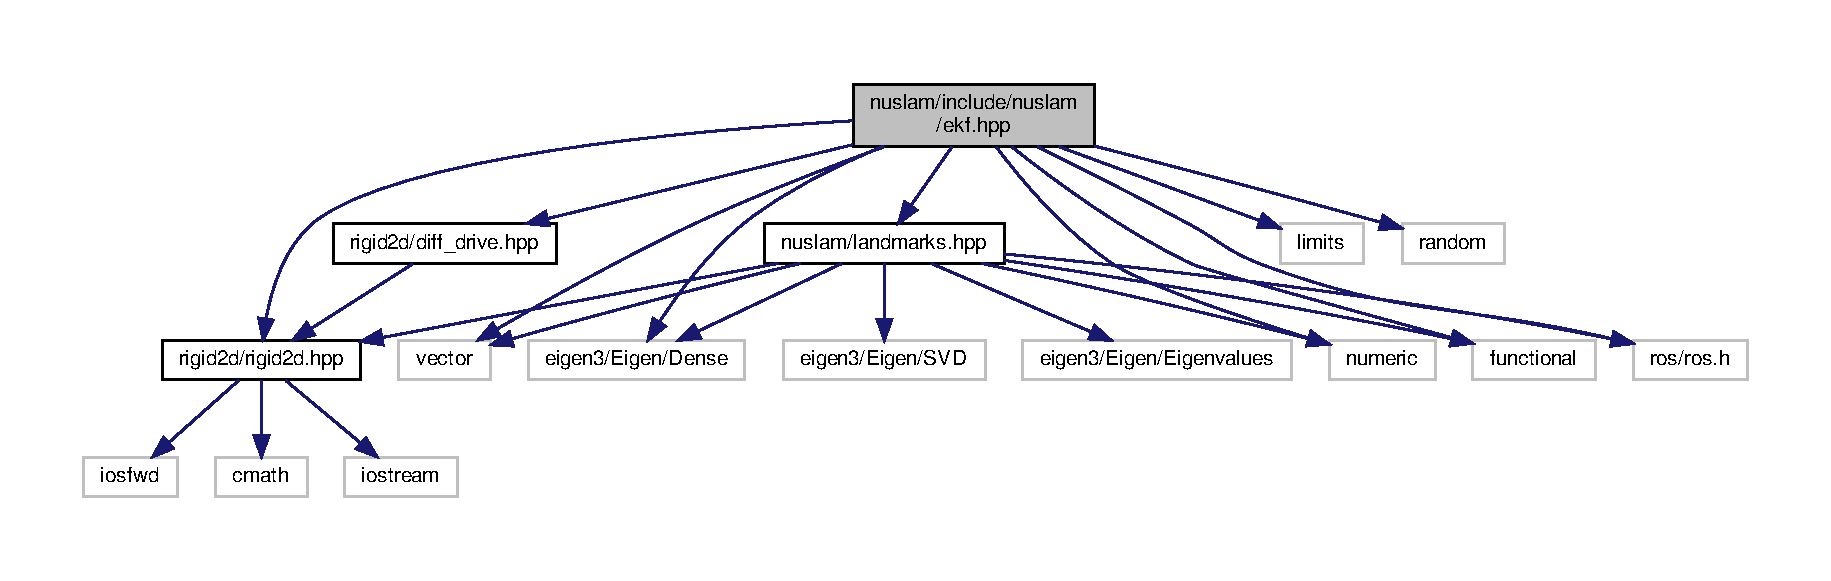
\includegraphics[width=350pt]{d0/dc6/ekf_8hpp__incl}
\end{center}
\end{figure}
This graph shows which files directly or indirectly include this file\+:\nopagebreak
\begin{figure}[H]
\begin{center}
\leavevmode
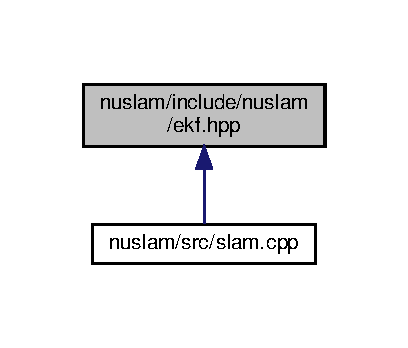
\includegraphics[width=196pt]{d8/dd5/ekf_8hpp__dep__incl}
\end{center}
\end{figure}
\subsection*{Classes}
\begin{DoxyCompactItemize}
\item 
struct \hyperlink{structnuslam_1_1CovarianceMatrix}{nuslam\+::\+Covariance\+Matrix}
\item 
struct \hyperlink{structnuslam_1_1ProcessNoise}{nuslam\+::\+Process\+Noise}
\item 
struct \hyperlink{structnuslam_1_1MeasurementNoise}{nuslam\+::\+Measurement\+Noise}
\item 
class \hyperlink{classnuslam_1_1EKF}{nuslam\+::\+E\+KF}
\begin{DoxyCompactList}\small\item\em handles model propagation for \hyperlink{classnuslam_1_1EKF}{E\+KF} S\+L\+AM \end{DoxyCompactList}\end{DoxyCompactItemize}
\subsection*{Functions}
\begin{DoxyCompactItemize}
\item 
std\+::mt19937 \& \hyperlink{ekf_8hpp_abbd1324d49509faf3e5d749aac18a8e5}{nuslam\+::get\+\_\+random} ()
\begin{DoxyCompactList}\small\item\em create random number generator with common seed \end{DoxyCompactList}\item 
Eigen\+::\+Vector\+Xd \hyperlink{ekf_8hpp_ad7de408dbbbab0e7ccd8ab5472de02d7}{nuslam\+::sample\+Normal\+Distribution} (int mtx\+\_\+dimension)
\begin{DoxyCompactList}\small\item\em sample normal distribution \end{DoxyCompactList}\item 
Eigen\+::\+Vector\+Xd \hyperlink{ekf_8hpp_aeb4d0c73a3d4fb1c60d70cb02a547f75}{nuslam\+::get\+Multivar\+Noise} (const Eigen\+::\+Matrix\+Xd \&noise\+\_\+mtx)
\begin{DoxyCompactList}\small\item\em returns noise for each dimension (x,y,theta) extracted from 3D normal distribution using Cholesky Decomposition \end{DoxyCompactList}\end{DoxyCompactItemize}


\subsection{Detailed Description}
Library E\+KF E\+KF detection and classification. 



\subsection{Function Documentation}
\mbox{\Hypertarget{ekf_8hpp_file_abbd1324d49509faf3e5d749aac18a8e5}\label{ekf_8hpp_file_abbd1324d49509faf3e5d749aac18a8e5}} 
\index{ekf.\+hpp@{ekf.\+hpp}!get\+\_\+random@{get\+\_\+random}}
\index{get\+\_\+random@{get\+\_\+random}!ekf.\+hpp@{ekf.\+hpp}}
\subsubsection{\texorpdfstring{get\+\_\+random()}{get\_random()}}
{\footnotesize\ttfamily std\+::mt19937 \& nuslam\+::get\+\_\+random (\begin{DoxyParamCaption}{ }\end{DoxyParamCaption})}



create random number generator with common seed 

\begin{DoxyReturn}{Returns}
number generator 
\end{DoxyReturn}
\mbox{\Hypertarget{ekf_8hpp_file_aeb4d0c73a3d4fb1c60d70cb02a547f75}\label{ekf_8hpp_file_aeb4d0c73a3d4fb1c60d70cb02a547f75}} 
\index{ekf.\+hpp@{ekf.\+hpp}!get\+Multivar\+Noise@{get\+Multivar\+Noise}}
\index{get\+Multivar\+Noise@{get\+Multivar\+Noise}!ekf.\+hpp@{ekf.\+hpp}}
\subsubsection{\texorpdfstring{get\+Multivar\+Noise()}{getMultivarNoise()}}
{\footnotesize\ttfamily Eigen\+::\+Vector\+Xd nuslam\+::get\+Multivar\+Noise (\begin{DoxyParamCaption}\item[{const Eigen\+::\+Matrix\+Xd \&}]{noise\+\_\+mtx }\end{DoxyParamCaption})}



returns noise for each dimension (x,y,theta) extracted from 3D normal distribution using Cholesky Decomposition 

\begin{DoxyReturn}{Returns}
noise matrix 
\end{DoxyReturn}
\mbox{\Hypertarget{ekf_8hpp_file_ad7de408dbbbab0e7ccd8ab5472de02d7}\label{ekf_8hpp_file_ad7de408dbbbab0e7ccd8ab5472de02d7}} 
\index{ekf.\+hpp@{ekf.\+hpp}!sample\+Normal\+Distribution@{sample\+Normal\+Distribution}}
\index{sample\+Normal\+Distribution@{sample\+Normal\+Distribution}!ekf.\+hpp@{ekf.\+hpp}}
\subsubsection{\texorpdfstring{sample\+Normal\+Distribution()}{sampleNormalDistribution()}}
{\footnotesize\ttfamily Eigen\+::\+Vector\+Xd nuslam\+::sample\+Normal\+Distribution (\begin{DoxyParamCaption}\item[{int}]{mtx\+\_\+dimension }\end{DoxyParamCaption})}



sample normal distribution 

\begin{DoxyReturn}{Returns}
noies vector 
\end{DoxyReturn}

\hypertarget{landmarks_8hpp}{}\section{nuslam/include/nuslam/landmarks.hpp File Reference}
\label{landmarks_8hpp}\index{nuslam/include/nuslam/landmarks.\+hpp@{nuslam/include/nuslam/landmarks.\+hpp}}


Library Landmarks landmark detection and classification.  


{\ttfamily \#include $<$rigid2d/rigid2d.\+hpp$>$}\newline
{\ttfamily \#include $<$vector$>$}\newline
{\ttfamily \#include $<$eigen3/\+Eigen/\+Dense$>$}\newline
{\ttfamily \#include $<$eigen3/\+Eigen/\+S\+VD$>$}\newline
{\ttfamily \#include $<$eigen3/\+Eigen/\+Eigenvalues$>$}\newline
{\ttfamily \#include $<$numeric$>$}\newline
{\ttfamily \#include $<$functional$>$}\newline
{\ttfamily \#include $<$ros/ros.\+h$>$}\newline
Include dependency graph for landmarks.\+hpp\+:
\nopagebreak
\begin{figure}[H]
\begin{center}
\leavevmode
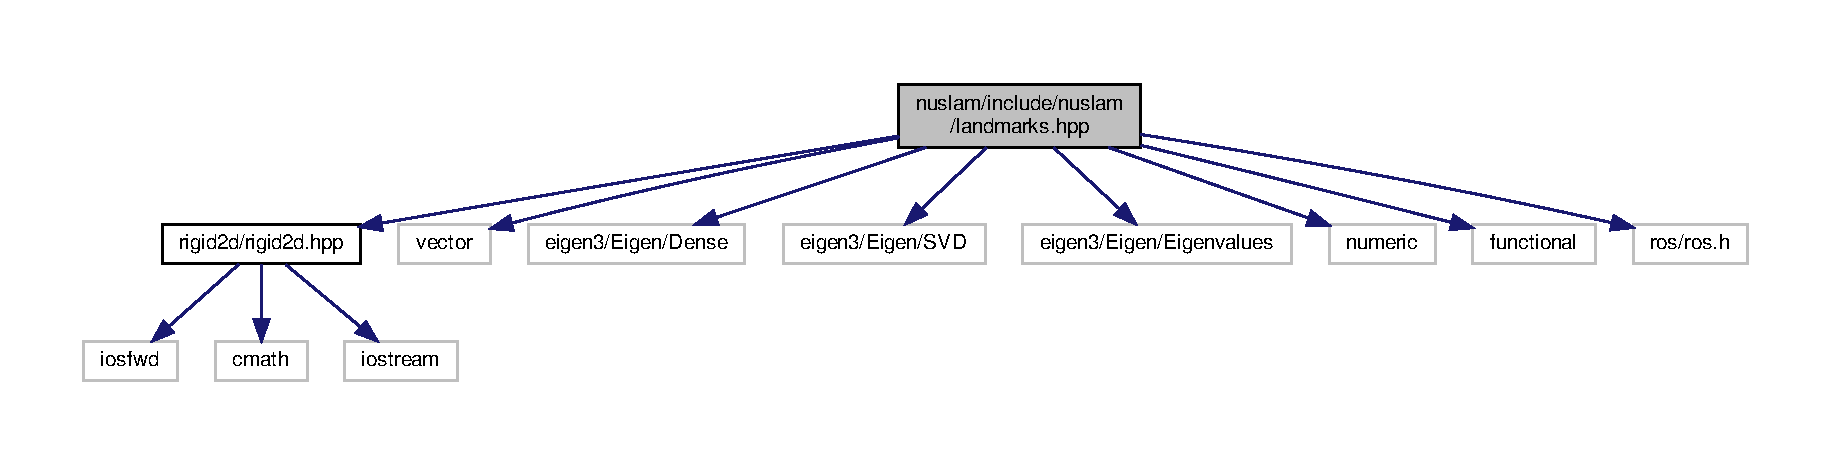
\includegraphics[width=350pt]{d4/d7b/landmarks_8hpp__incl}
\end{center}
\end{figure}
This graph shows which files directly or indirectly include this file\+:
\nopagebreak
\begin{figure}[H]
\begin{center}
\leavevmode
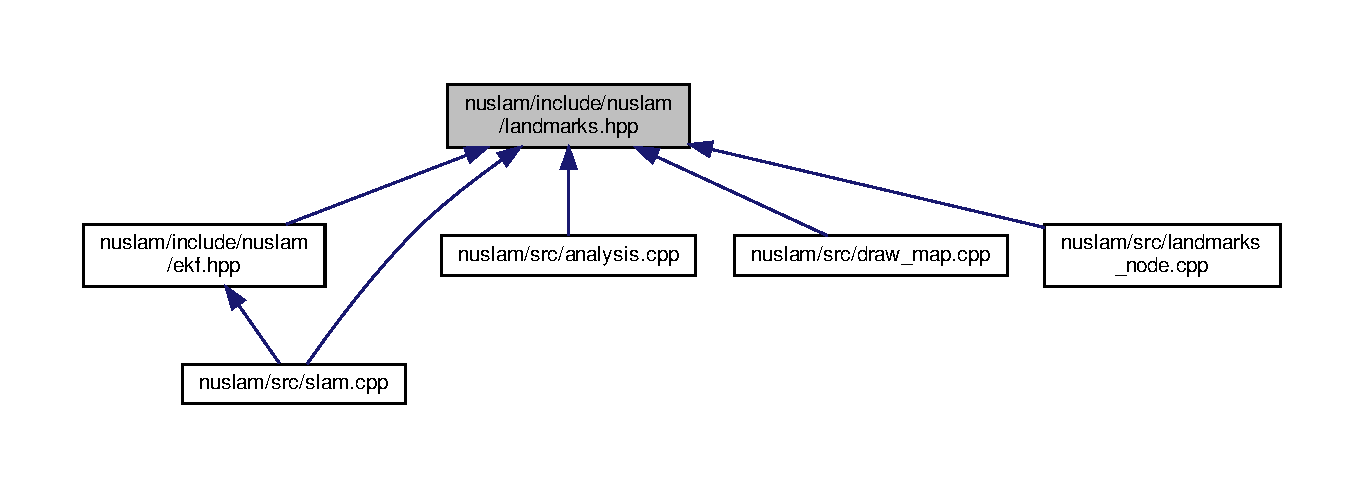
\includegraphics[width=350pt]{d6/dc7/landmarks_8hpp__dep__incl}
\end{center}
\end{figure}
\subsection*{Classes}
\begin{DoxyCompactItemize}
\item 
struct \hyperlink{structnuslam_1_1RangeBear}{nuslam\+::\+Range\+Bear}
\item 
struct \hyperlink{structnuslam_1_1Point}{nuslam\+::\+Point}
\item 
class \hyperlink{classnuslam_1_1Landmark}{nuslam\+::\+Landmark}
\begin{DoxyCompactList}\small\item\em create a \hyperlink{classnuslam_1_1Landmark}{Landmark} with pose relative to turtlebot3 \end{DoxyCompactList}\end{DoxyCompactItemize}
\subsection*{Functions}
\begin{DoxyCompactItemize}
\item 
Range\+Bear \hyperlink{landmarks_8hpp_a89c1543adf36dbb0ab21be32cfd40d13}{nuslam\+::cartesian\+To\+Polar} (const Vector2D \&pose)
\begin{DoxyCompactList}\small\item\em gets polar coordinates from cartesian coodinates \end{DoxyCompactList}\item 
Vector2D \hyperlink{landmarks_8hpp_aa8d74c83e481a6b574639b241b925f2f}{nuslam\+::polar\+To\+Cartesian} (const Range\+Bear \&range\+\_\+bear)
\begin{DoxyCompactList}\small\item\em gets cartesian coordinates from polar coodinates \end{DoxyCompactList}\end{DoxyCompactItemize}


\subsection{Detailed Description}
Library Landmarks landmark detection and classification. 



\subsection{Function Documentation}
\mbox{\Hypertarget{landmarks_8hpp_file_a89c1543adf36dbb0ab21be32cfd40d13}\label{landmarks_8hpp_file_a89c1543adf36dbb0ab21be32cfd40d13}} 
\index{landmarks.\+hpp@{landmarks.\+hpp}!cartesian\+To\+Polar@{cartesian\+To\+Polar}}
\index{cartesian\+To\+Polar@{cartesian\+To\+Polar}!landmarks.\+hpp@{landmarks.\+hpp}}
\subsubsection{\texorpdfstring{cartesian\+To\+Polar()}{cartesianToPolar()}}
{\footnotesize\ttfamily Range\+Bear nuslam\+::cartesian\+To\+Polar (\begin{DoxyParamCaption}\item[{const \hyperlink{structrigid2d_1_1Vector2D}{Vector2D} \&}]{pose }\end{DoxyParamCaption})}



gets polar coordinates from cartesian coodinates 


\begin{DoxyParams}{Parameters}
{\em pose} & containing x and y position relative to robot \\
\hline
\end{DoxyParams}
\begin{DoxyReturn}{Returns}
Range\+Bear struct containing range and bearing 
\end{DoxyReturn}
\mbox{\Hypertarget{landmarks_8hpp_file_aa8d74c83e481a6b574639b241b925f2f}\label{landmarks_8hpp_file_aa8d74c83e481a6b574639b241b925f2f}} 
\index{landmarks.\+hpp@{landmarks.\+hpp}!polar\+To\+Cartesian@{polar\+To\+Cartesian}}
\index{polar\+To\+Cartesian@{polar\+To\+Cartesian}!landmarks.\+hpp@{landmarks.\+hpp}}
\subsubsection{\texorpdfstring{polar\+To\+Cartesian()}{polarToCartesian()}}
{\footnotesize\ttfamily Vector2D nuslam\+::polar\+To\+Cartesian (\begin{DoxyParamCaption}\item[{const \hyperlink{structnuslam_1_1RangeBear}{Range\+Bear} \&}]{range\+\_\+bear }\end{DoxyParamCaption})}



gets cartesian coordinates from polar coodinates 


\begin{DoxyParams}{Parameters}
{\em Range\+Bear} & struct containing range and bearing \\
\hline
\end{DoxyParams}
\begin{DoxyReturn}{Returns}
Vector2D containing cartesian coordinates 
\end{DoxyReturn}

\hypertarget{analysis_8cpp}{}\section{nuslam/src/analysis.cpp File Reference}
\label{analysis_8cpp}\index{nuslam/src/analysis.\+cpp@{nuslam/src/analysis.\+cpp}}


Publishes coordinates of available landmarks straight from gazebo (no noise) relative to robot.  


{\ttfamily \#include $<$ros/ros.\+h$>$}\newline
{\ttfamily \#include $<$std\+\_\+srvs/\+Empty.\+h$>$}\newline
{\ttfamily \#include $<$math.\+h$>$}\newline
{\ttfamily \#include $<$string$>$}\newline
{\ttfamily \#include $<$vector$>$}\newline
{\ttfamily \#include $<$boost/iterator/zip\+\_\+iterator.\+hpp$>$}\newline
{\ttfamily \#include \char`\"{}nuslam/\+Turtle\+Map.\+h\char`\"{}}\newline
{\ttfamily \#include $<$gazebo\+\_\+msgs/\+Model\+States.\+h$>$}\newline
{\ttfamily \#include $<$geometry\+\_\+msgs/\+Pose.\+h$>$}\newline
{\ttfamily \#include $<$functional$>$}\newline
{\ttfamily \#include $<$algorithm$>$}\newline
{\ttfamily \#include \char`\"{}nuslam/landmarks.\+hpp\char`\"{}}\newline
{\ttfamily \#include $<$tf2/\+Linear\+Math/\+Quaternion.\+h$>$}\newline
{\ttfamily \#include $<$tf2/\+Linear\+Math/\+Matrix3x3.\+h$>$}\newline
Include dependency graph for analysis.\+cpp\+:\nopagebreak
\begin{figure}[H]
\begin{center}
\leavevmode
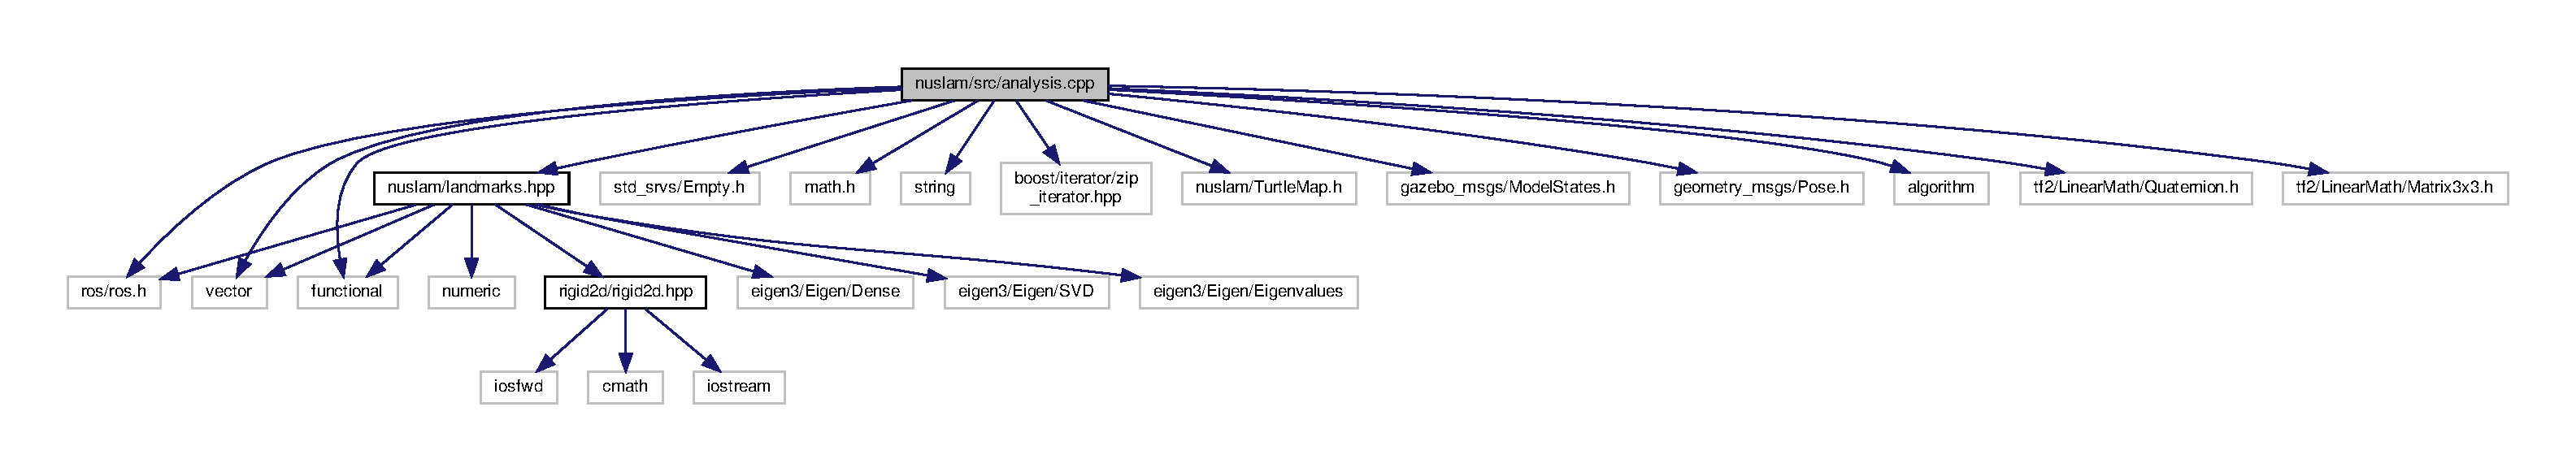
\includegraphics[width=350pt]{d5/dbb/analysis_8cpp__incl}
\end{center}
\end{figure}
\subsection*{Functions}
\begin{DoxyCompactItemize}
\item 
void \hyperlink{analysis_8cpp_adbc02ba8fb4d3eeee5b172ca53ebf61c}{gazebo\+\_\+callback} (const gazebo\+\_\+msgs\+::\+Model\+States \&model)
\item 
\mbox{\Hypertarget{analysis_8cpp_a3c04138a5bfe5d72780bb7e82a18e627}\label{analysis_8cpp_a3c04138a5bfe5d72780bb7e82a18e627}} 
int \hyperlink{analysis_8cpp_a3c04138a5bfe5d72780bb7e82a18e627}{main} (int argc, char $\ast$$\ast$argv)
\begin{DoxyCompactList}\small\item\em The Main Function ///. \end{DoxyCompactList}\end{DoxyCompactItemize}
\subsection*{Variables}
\begin{DoxyCompactItemize}
\item 
\mbox{\Hypertarget{analysis_8cpp_a3ee0ad2c2fb892e39c44a42e14f18ce4}\label{analysis_8cpp_a3ee0ad2c2fb892e39c44a42e14f18ce4}} 
bool {\bfseries callback\+\_\+flag} = false
\item 
\mbox{\Hypertarget{analysis_8cpp_a479b2db06058877d6bc4eea716274724}\label{analysis_8cpp_a479b2db06058877d6bc4eea716274724}} 
nuslam\+::\+Turtle\+Map {\bfseries map}
\item 
\mbox{\Hypertarget{analysis_8cpp_a4df94e397e7df41d9894ed8e0a069ae1}\label{analysis_8cpp_a4df94e397e7df41d9894ed8e0a069ae1}} 
std\+::string {\bfseries landmark\+\_\+name} = \char`\"{}cylinder\char`\"{}
\item 
\mbox{\Hypertarget{analysis_8cpp_a3b5bbcd0e93dca30ec3cc609f1f5373e}\label{analysis_8cpp_a3b5bbcd0e93dca30ec3cc609f1f5373e}} 
std\+::string {\bfseries robot\+\_\+name} = \char`\"{}diff\+\_\+drive\char`\"{}
\end{DoxyCompactItemize}


\subsection{Detailed Description}
Publishes coordinates of available landmarks straight from gazebo (no noise) relative to robot. 

P\+A\+R\+A\+M\+E\+T\+E\+RS\+: callback\+\_\+flag (bool)\+: specifies whether to draw landmarks from based on callback trigger map (nuslam\+::\+Turtle\+Map)\+: stores lists of x,y coordinates and radii of landmarks to publish frequency (double)\+: frequency of control loop. frame\+\_\+id\+\_\+ (string)\+: frame with respect to which landmark coordinates are published (\char`\"{}base\+\_\+scan\char`\"{} here)

P\+U\+B\+L\+I\+S\+H\+ES\+: landmarks (nuslam\+::\+Turtle\+Map)\+: publishes Turtle\+Map message containing landmark coordinates (x,y) and radii

S\+U\+B\+S\+C\+R\+I\+B\+ES\+: /gazebo/model\+\_\+states (gazebo\+\_\+msgs\+::\+Model\+States) to read robot and landmark Poses

F\+U\+N\+C\+T\+I\+O\+NS\+: gazebo\+\_\+callback (void)\+: callback for /gazebo/model\+\_\+states subscriber to get landmark coordinates relative to robot 

\subsection{Function Documentation}
\mbox{\Hypertarget{analysis_8cpp_adbc02ba8fb4d3eeee5b172ca53ebf61c}\label{analysis_8cpp_adbc02ba8fb4d3eeee5b172ca53ebf61c}} 
\index{analysis.\+cpp@{analysis.\+cpp}!gazebo\+\_\+callback@{gazebo\+\_\+callback}}
\index{gazebo\+\_\+callback@{gazebo\+\_\+callback}!analysis.\+cpp@{analysis.\+cpp}}
\subsubsection{\texorpdfstring{gazebo\+\_\+callback()}{gazebo\_callback()}}
{\footnotesize\ttfamily void gazebo\+\_\+callback (\begin{DoxyParamCaption}\item[{const gazebo\+\_\+msgs\+::\+Model\+States \&}]{model }\end{DoxyParamCaption})}

extract turtlebot pose and landmark poses from Model\+States, then computes relative cartesian coordinates to publish as Turtle\+Map message with arbitrary radius 
\begin{DoxyParams}{Parameters}
{\em gazebo\+\_\+msgs\+::\+Model\+States,containing} & the pose of all models in the environment \\
\hline
\end{DoxyParams}

\hypertarget{draw__map_8cpp}{}\section{nuslam/src/draw\+\_\+map.cpp File Reference}
\label{draw__map_8cpp}\index{nuslam/src/draw\+\_\+map.\+cpp@{nuslam/src/draw\+\_\+map.\+cpp}}


Receives Turtle\+Map data and publishes markers to R\+Viz which indicate landmark estimations.  


{\ttfamily \#include $<$ros/ros.\+h$>$}\newline
{\ttfamily \#include $<$std\+\_\+srvs/\+Empty.\+h$>$}\newline
{\ttfamily \#include $<$visualization\+\_\+msgs/\+Marker.\+h$>$}\newline
{\ttfamily \#include $<$sensor\+\_\+msgs/\+Laser\+Scan.\+h$>$}\newline
{\ttfamily \#include $<$math.\+h$>$}\newline
{\ttfamily \#include $<$string$>$}\newline
{\ttfamily \#include $<$vector$>$}\newline
{\ttfamily \#include $<$boost/iterator/zip\+\_\+iterator.\+hpp$>$}\newline
{\ttfamily \#include \char`\"{}nuslam/landmarks.\+hpp\char`\"{}}\newline
{\ttfamily \#include \char`\"{}nuslam/\+Turtle\+Map.\+h\char`\"{}}\newline
{\ttfamily \#include $<$functional$>$}\newline
Include dependency graph for draw\+\_\+map.\+cpp\+:\nopagebreak
\begin{figure}[H]
\begin{center}
\leavevmode
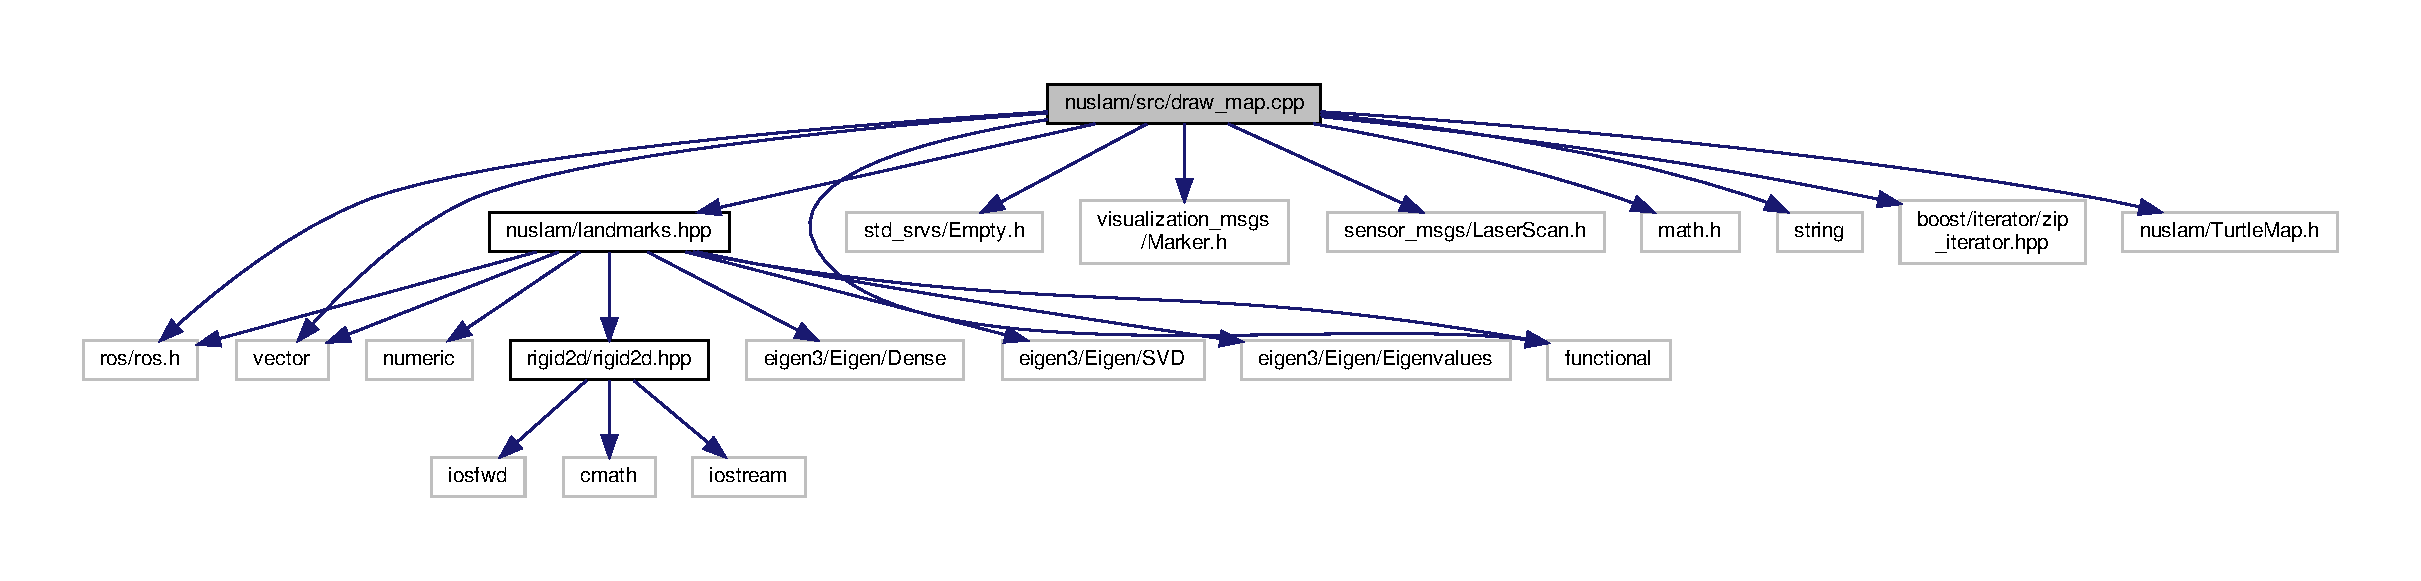
\includegraphics[width=350pt]{df/de5/draw__map_8cpp__incl}
\end{center}
\end{figure}
\subsection*{Functions}
\begin{DoxyCompactItemize}
\item 
void \hyperlink{draw__map_8cpp_a7b3e91ec368e7d5a4082f972e7cdd0a2}{map\+Callback} (const nuslam\+::\+Turtle\+Map \&map)
\item 
\mbox{\Hypertarget{draw__map_8cpp_a3c04138a5bfe5d72780bb7e82a18e627}\label{draw__map_8cpp_a3c04138a5bfe5d72780bb7e82a18e627}} 
int \hyperlink{draw__map_8cpp_a3c04138a5bfe5d72780bb7e82a18e627}{main} (int argc, char $\ast$$\ast$argv)
\begin{DoxyCompactList}\small\item\em The Main Function ///. \end{DoxyCompactList}\end{DoxyCompactItemize}
\subsection*{Variables}
\begin{DoxyCompactItemize}
\item 
\mbox{\Hypertarget{draw__map_8cpp_a3ee0ad2c2fb892e39c44a42e14f18ce4}\label{draw__map_8cpp_a3ee0ad2c2fb892e39c44a42e14f18ce4}} 
bool {\bfseries callback\+\_\+flag} = false
\item 
\mbox{\Hypertarget{draw__map_8cpp_add282c3ccb897740380532389b28dded}\label{draw__map_8cpp_add282c3ccb897740380532389b28dded}} 
nuslam\+::\+Turtle\+Map {\bfseries global\+\_\+map}
\end{DoxyCompactItemize}


\subsection{Detailed Description}
Receives Turtle\+Map data and publishes markers to R\+Viz which indicate landmark estimations. 

P\+A\+R\+A\+M\+E\+T\+E\+RS\+: callback\+\_\+flag (bool)\+: specifies whether to draw landmarks from based on callback trigger global\+\_\+map (nuslam\+::\+Turtle\+Map)\+: stores lists of x,y coordinates and radii of landmarks to publish frequency (double)\+: frequency of control loop. color (string)\+: \char`\"{}gazebo\char`\"{}, \char`\"{}scan\char`\"{}, or \char`\"{}slam\char`\"{} determines color and size of markers for clarity

P\+U\+B\+L\+I\+S\+H\+ES\+: scan/marker (visualization\+\_\+msgs\+::\+Marker)\+: publishes markers to indicate detected landmark positions

S\+U\+B\+S\+C\+R\+I\+B\+ES\+: /landmarks\+\_\+node/landmarks (nuslam\+::\+Turtle\+Map), stores lists of x,y coordinates and radii of detected landmarks

F\+U\+N\+C\+T\+I\+O\+NS\+: map\+Callback (void)\+: callback for /landmarks\+\_\+node/landmarks subscriber, which stores Turtle\+Map data for exraction 

\subsection{Function Documentation}
\mbox{\Hypertarget{draw__map_8cpp_a7b3e91ec368e7d5a4082f972e7cdd0a2}\label{draw__map_8cpp_a7b3e91ec368e7d5a4082f972e7cdd0a2}} 
\index{draw\+\_\+map.\+cpp@{draw\+\_\+map.\+cpp}!map\+Callback@{map\+Callback}}
\index{map\+Callback@{map\+Callback}!draw\+\_\+map.\+cpp@{draw\+\_\+map.\+cpp}}
\subsubsection{\texorpdfstring{map\+Callback()}{mapCallback()}}
{\footnotesize\ttfamily void map\+Callback (\begin{DoxyParamCaption}\item[{const nuslam\+::\+Turtle\+Map \&}]{map }\end{DoxyParamCaption})}

store Turtle\+Map data for converting into marker coordinates 
\begin{DoxyParams}{Parameters}
{\em nuslam\+::\+Turtle\+Map,which} & stores lists of x,y coordinates and radii of detected landmarks \\
\hline
\end{DoxyParams}

\hypertarget{landmarks__node_8cpp}{}\section{nuslam/src/landmarks\+\_\+node.cpp File Reference}
\label{landmarks__node_8cpp}\index{nuslam/src/landmarks\+\_\+node.\+cpp@{nuslam/src/landmarks\+\_\+node.\+cpp}}


Interprets Laser\+Scan data and detects and publishes attributes of discovered landmarks.  


{\ttfamily \#include $<$ros/ros.\+h$>$}\newline
{\ttfamily \#include $<$std\+\_\+srvs/\+Empty.\+h$>$}\newline
{\ttfamily \#include $<$visualization\+\_\+msgs/\+Marker.\+h$>$}\newline
{\ttfamily \#include $<$sensor\+\_\+msgs/\+Laser\+Scan.\+h$>$}\newline
{\ttfamily \#include $<$sensor\+\_\+msgs/\+Point\+Cloud.\+h$>$}\newline
{\ttfamily \#include $<$geometry\+\_\+msgs/\+Point32.\+h$>$}\newline
{\ttfamily \#include $<$math.\+h$>$}\newline
{\ttfamily \#include $<$string$>$}\newline
{\ttfamily \#include $<$vector$>$}\newline
{\ttfamily \#include $<$boost/iterator/zip\+\_\+iterator.\+hpp$>$}\newline
{\ttfamily \#include \char`\"{}nuslam/landmarks.\+hpp\char`\"{}}\newline
{\ttfamily \#include \char`\"{}nuslam/\+Turtle\+Map.\+h\char`\"{}}\newline
{\ttfamily \#include $<$functional$>$}\newline
Include dependency graph for landmarks\+\_\+node.\+cpp\+:
\nopagebreak
\begin{figure}[H]
\begin{center}
\leavevmode
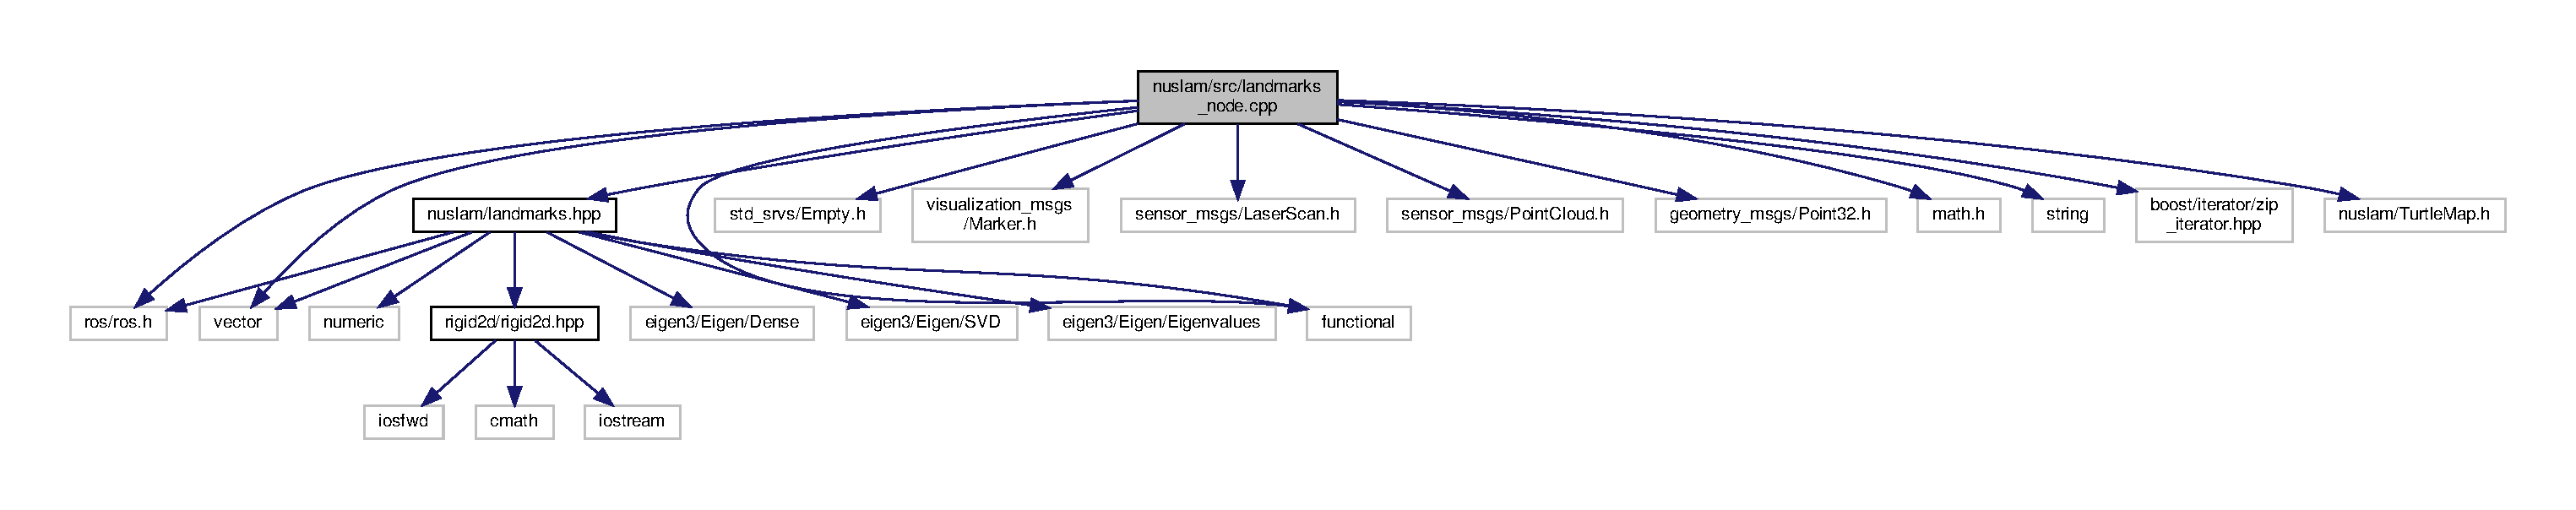
\includegraphics[width=350pt]{d6/d59/landmarks__node_8cpp__incl}
\end{center}
\end{figure}
\subsection*{Functions}
\begin{DoxyCompactItemize}
\item 
void \hyperlink{landmarks__node_8cpp_a2ba8b69ec42a8dcac8c1f47c66c3f87b}{scan\+\_\+callback} (const sensor\+\_\+msgs\+::\+Laser\+Scan \&lsr)
\item 
\mbox{\Hypertarget{landmarks__node_8cpp_a3c04138a5bfe5d72780bb7e82a18e627}\label{landmarks__node_8cpp_a3c04138a5bfe5d72780bb7e82a18e627}} 
int \hyperlink{landmarks__node_8cpp_a3c04138a5bfe5d72780bb7e82a18e627}{main} (int argc, char $\ast$$\ast$argv)
\begin{DoxyCompactList}\small\item\em The Main Function ///. \end{DoxyCompactList}\end{DoxyCompactItemize}
\subsection*{Variables}
\begin{DoxyCompactItemize}
\item 
\mbox{\Hypertarget{landmarks__node_8cpp_ad7f9420c5db55e41dcaf2e64df8153e0}\label{landmarks__node_8cpp_ad7f9420c5db55e41dcaf2e64df8153e0}} 
double {\bfseries threshold\+\_\+} = 0.\+15
\item 
\mbox{\Hypertarget{landmarks__node_8cpp_a3ee0ad2c2fb892e39c44a42e14f18ce4}\label{landmarks__node_8cpp_a3ee0ad2c2fb892e39c44a42e14f18ce4}} 
bool {\bfseries callback\+\_\+flag} = false
\item 
\mbox{\Hypertarget{landmarks__node_8cpp_a479b2db06058877d6bc4eea716274724}\label{landmarks__node_8cpp_a479b2db06058877d6bc4eea716274724}} 
nuslam\+::\+Turtle\+Map {\bfseries map}
\item 
\mbox{\Hypertarget{landmarks__node_8cpp_a258c4690fc0d9b08db17b585fc214738}\label{landmarks__node_8cpp_a258c4690fc0d9b08db17b585fc214738}} 
sensor\+\_\+msgs\+::\+Point\+Cloud {\bfseries pc}
\end{DoxyCompactItemize}


\subsection{Detailed Description}
Interprets Laser\+Scan data and detects and publishes attributes of discovered landmarks. 

P\+A\+R\+A\+M\+E\+T\+E\+RS\+: threshold (double)\+: used to determine whether two points from Laser\+Scan belong to one cluster callback\+\_\+flag (bool)\+: specifies whether to publish landmarks based on callback trigger pc (sensor\+\_\+msgs\+::\+Point\+Cloud)\+: contains interpreted pointcloud which is published for debugging purposes map (nuslam\+::\+Turtle\+Map)\+: stores lists of x,y coordinates and radii of detected landmarks frequency (double)\+: frequency of control loop. frame\+\_\+id\+\_\+ (string)\+: frame ID of discovered landmarks (in this case, relative to base\+\_\+scan)

P\+U\+B\+L\+I\+S\+H\+ES\+: landmarks (nuslam\+::\+Turtle\+Map)\+: publishes Turtle\+Map message containing landmark coordinates (x,y) and radii pointcloud (sensor\+\_\+msgs\+::\+Point\+Cloud)\+: publishes Point\+Cloud for visualization in R\+Viz for debugging purposees

S\+U\+B\+S\+C\+R\+I\+B\+ES\+: /scan (sensor\+\_\+msgs\+::\+Laser\+Scan), which contains data with which it is possible to extract range,bearing measurements

F\+U\+N\+C\+T\+I\+O\+NS\+: scan\+\_\+callback (void)\+: callback for /scan subscriber, which processes Laser\+Scan data and detects landmarks 

\subsection{Function Documentation}
\mbox{\Hypertarget{landmarks__node_8cpp_a2ba8b69ec42a8dcac8c1f47c66c3f87b}\label{landmarks__node_8cpp_a2ba8b69ec42a8dcac8c1f47c66c3f87b}} 
\index{landmarks\+\_\+node.\+cpp@{landmarks\+\_\+node.\+cpp}!scan\+\_\+callback@{scan\+\_\+callback}}
\index{scan\+\_\+callback@{scan\+\_\+callback}!landmarks\+\_\+node.\+cpp@{landmarks\+\_\+node.\+cpp}}
\subsubsection{\texorpdfstring{scan\+\_\+callback()}{scan\_callback()}}
{\footnotesize\ttfamily void scan\+\_\+callback (\begin{DoxyParamCaption}\item[{const sensor\+\_\+msgs\+::\+Laser\+Scan \&}]{lsr }\end{DoxyParamCaption})}

forms clusters from Laser\+Scan data and fits circles to them before assessing whether or not they are landmarks (or walls) 
\begin{DoxyParams}{Parameters}
{\em sensor\+\_\+msgs\+::\+Laser\+Scan,which} & contains data with which it is possible to extract range,bearing measurements \\
\hline
\end{DoxyParams}

\hypertarget{slam_8cpp}{}\section{nuslam/src/slam.cpp File Reference}
\label{slam_8cpp}\index{nuslam/src/slam.\+cpp@{nuslam/src/slam.\+cpp}}


Main\+: Publishes Odometry messages for diff drive robot using Extended Kalman Filter S\+L\+AM.  


{\ttfamily \#include $<$ros/ros.\+h$>$}\newline
{\ttfamily \#include $<$sensor\+\_\+msgs/\+Joint\+State.\+h$>$}\newline
{\ttfamily \#include $<$nav\+\_\+msgs/\+Odometry.\+h$>$}\newline
{\ttfamily \#include $<$tf2/\+Linear\+Math/\+Quaternion.\+h$>$}\newline
{\ttfamily \#include $<$tf2\+\_\+ros/transform\+\_\+broadcaster.\+h$>$}\newline
{\ttfamily \#include $<$tf2\+\_\+geometry\+\_\+msgs/tf2\+\_\+geometry\+\_\+msgs.\+h$>$}\newline
{\ttfamily \#include \char`\"{}rigid2d/\+Set\+Pose.\+h\char`\"{}}\newline
{\ttfamily \#include $<$string$>$}\newline
{\ttfamily \#include \char`\"{}nuslam/landmarks.\+hpp\char`\"{}}\newline
{\ttfamily \#include \char`\"{}nuslam/ekf.\+hpp\char`\"{}}\newline
{\ttfamily \#include \char`\"{}nuslam/\+Turtle\+Map.\+h\char`\"{}}\newline
{\ttfamily \#include \char`\"{}rigid2d/rigid2d.\+hpp\char`\"{}}\newline
{\ttfamily \#include \char`\"{}rigid2d/diff\+\_\+drive.\+hpp\char`\"{}}\newline
Include dependency graph for slam.\+cpp\+:
\nopagebreak
\begin{figure}[H]
\begin{center}
\leavevmode
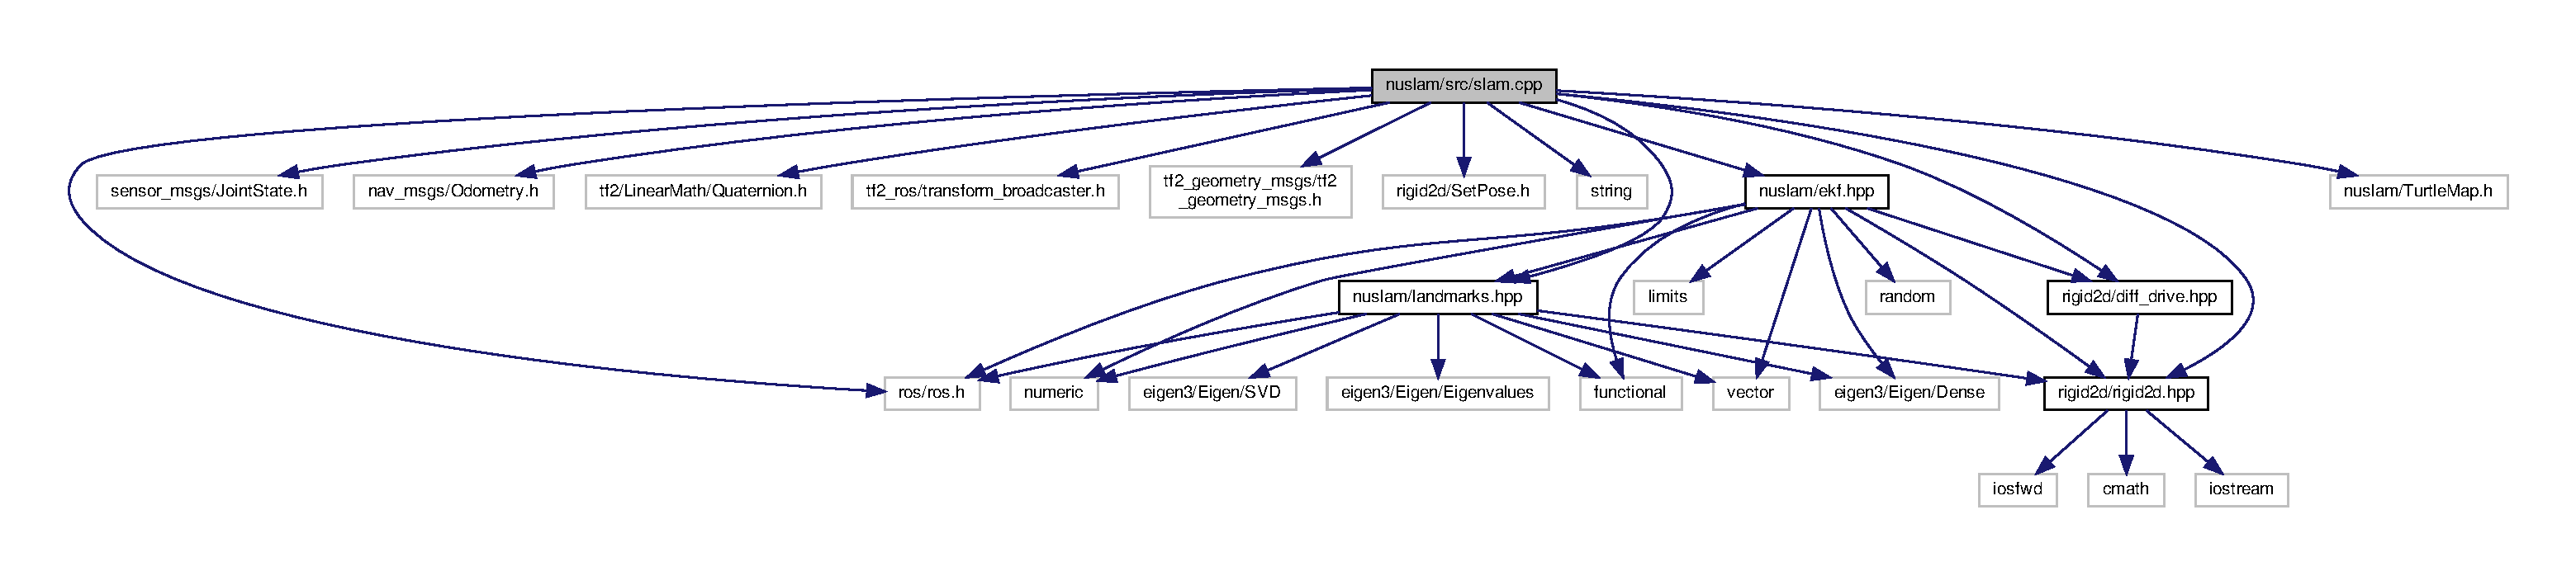
\includegraphics[width=350pt]{d2/d57/slam_8cpp__incl}
\end{center}
\end{figure}
\subsection*{Functions}
\begin{DoxyCompactItemize}
\item 
void \hyperlink{slam_8cpp_a8f0c3d2ac4fed55d807bd69afb5243b4}{js\+\_\+callback} (const sensor\+\_\+msgs\+::\+Joint\+State\+::\+Const\+Ptr \&js)
\item 
void \hyperlink{slam_8cpp_a7c7402381f220beb7cf9b6be1a846a0d}{landmark\+\_\+callback} (const nuslam\+::\+Turtle\+Map \&map)
\item 
bool \hyperlink{slam_8cpp_adb6929707bcc4d4fb332481cb33e4f2b}{set\+\_\+pose\+Callback} (rigid2d\+::\+Set\+Pose\+::\+Request \&req, rigid2d\+::\+Set\+Pose\+::\+Response \&res)
\begin{DoxyCompactList}\small\item\em set\+\_\+pose service callback. Sets the turtlebot\textquotesingle{}s pose belief to desired value. \end{DoxyCompactList}\item 
\mbox{\Hypertarget{slam_8cpp_a3c04138a5bfe5d72780bb7e82a18e627}\label{slam_8cpp_a3c04138a5bfe5d72780bb7e82a18e627}} 
int \hyperlink{slam_8cpp_a3c04138a5bfe5d72780bb7e82a18e627}{main} (int argc, char $\ast$$\ast$argv)
\begin{DoxyCompactList}\small\item\em The Main Function ///. \end{DoxyCompactList}\end{DoxyCompactItemize}
\subsection*{Variables}
\begin{DoxyCompactItemize}
\item 
\mbox{\Hypertarget{slam_8cpp_ad1ee493a9c3d90ec79d68e9de39a0d62}\label{slam_8cpp_ad1ee493a9c3d90ec79d68e9de39a0d62}} 
float {\bfseries wl\+\_\+enc} = 0
\item 
\mbox{\Hypertarget{slam_8cpp_a82d2473bdd4614b5a4532a95a0382487}\label{slam_8cpp_a82d2473bdd4614b5a4532a95a0382487}} 
float {\bfseries wr\+\_\+enc} = 0
\item 
\mbox{\Hypertarget{slam_8cpp_a9cac548254b5baa18c6e6234daf6b363}\label{slam_8cpp_a9cac548254b5baa18c6e6234daf6b363}} 
float {\bfseries ekf\+\_\+wl\+\_\+enc} = 0
\item 
\mbox{\Hypertarget{slam_8cpp_a0f595671e79941a5327ce59a25c848af}\label{slam_8cpp_a0f595671e79941a5327ce59a25c848af}} 
float {\bfseries ekf\+\_\+wr\+\_\+enc} = 0
\item 
\mbox{\Hypertarget{slam_8cpp_abb35a308e88b2a5d113795948e6273a3}\label{slam_8cpp_abb35a308e88b2a5d113795948e6273a3}} 
\hyperlink{classrigid2d_1_1Twist2D}{rigid2d\+::\+Twist2D} {\bfseries Vb}
\item 
\mbox{\Hypertarget{slam_8cpp_a002f817728ce76d60fecd0d2b5bcd214}\label{slam_8cpp_a002f817728ce76d60fecd0d2b5bcd214}} 
\hyperlink{structrigid2d_1_1WheelVelocities}{rigid2d\+::\+Wheel\+Velocities} {\bfseries w\+\_\+vel}
\item 
\mbox{\Hypertarget{slam_8cpp_aabf3dfeb602efbe1bc76a7918ae6e838}\label{slam_8cpp_aabf3dfeb602efbe1bc76a7918ae6e838}} 
\hyperlink{structrigid2d_1_1Pose2D}{rigid2d\+::\+Pose2D} {\bfseries reset\+\_\+pose}
\item 
\mbox{\Hypertarget{slam_8cpp_aae05b70475acb90fabcbcb02075b4a5c}\label{slam_8cpp_aae05b70475acb90fabcbcb02075b4a5c}} 
\hyperlink{classrigid2d_1_1DiffDrive}{rigid2d\+::\+Diff\+Drive} {\bfseries driver}
\item 
\mbox{\Hypertarget{slam_8cpp_a0f9be3dafe77e9ce1672b5991913de9c}\label{slam_8cpp_a0f9be3dafe77e9ce1672b5991913de9c}} 
\hyperlink{classrigid2d_1_1DiffDrive}{rigid2d\+::\+Diff\+Drive} {\bfseries ekf\+\_\+driver}
\item 
\mbox{\Hypertarget{slam_8cpp_a3ee0ad2c2fb892e39c44a42e14f18ce4}\label{slam_8cpp_a3ee0ad2c2fb892e39c44a42e14f18ce4}} 
bool {\bfseries callback\+\_\+flag} = false
\item 
\mbox{\Hypertarget{slam_8cpp_aec95f3184024dd2d359b2aed43355edd}\label{slam_8cpp_aec95f3184024dd2d359b2aed43355edd}} 
bool {\bfseries landmark\+\_\+flag} = false
\item 
\mbox{\Hypertarget{slam_8cpp_a766d6358d6980b16819f330ea0160e5d}\label{slam_8cpp_a766d6358d6980b16819f330ea0160e5d}} 
bool {\bfseries odom\+\_\+flag} = false
\item 
\mbox{\Hypertarget{slam_8cpp_a13c6e8170f4eaffabda3cd95e02d139c}\label{slam_8cpp_a13c6e8170f4eaffabda3cd95e02d139c}} 
bool {\bfseries service\+\_\+flag} = false
\item 
\mbox{\Hypertarget{slam_8cpp_a031d256a1ed5f4d7ff27d5bb5ae8eba1}\label{slam_8cpp_a031d256a1ed5f4d7ff27d5bb5ae8eba1}} 
\hyperlink{classnuslam_1_1EKF}{nuslam\+::\+E\+KF} {\bfseries ekf}
\item 
\mbox{\Hypertarget{slam_8cpp_a95ebc576c07050b8e37cbcddffab08e1}\label{slam_8cpp_a95ebc576c07050b8e37cbcddffab08e1}} 
std\+::vector$<$ double $>$ {\bfseries radii}
\item 
\mbox{\Hypertarget{slam_8cpp_a0c7bee542075db748c57c5b4604c062c}\label{slam_8cpp_a0c7bee542075db748c57c5b4604c062c}} 
std\+::vector$<$ double $>$ {\bfseries x\+\_\+pts}
\item 
\mbox{\Hypertarget{slam_8cpp_acbd567921dc5721dadae3d37c73d4c26}\label{slam_8cpp_acbd567921dc5721dadae3d37c73d4c26}} 
std\+::vector$<$ double $>$ {\bfseries y\+\_\+pts}
\end{DoxyCompactItemize}


\subsection{Detailed Description}
Main\+: Publishes Odometry messages for diff drive robot using Extended Kalman Filter S\+L\+AM. 

P\+A\+R\+A\+M\+E\+T\+E\+RS\+: o\+\_\+fid\+\_\+ (string)\+: parent frame ID for the published tf transform o\+\_\+fid\+\_\+ (string)\+: child frame ID for the published tf transform wbase\+\_\+ (float)\+: wheel base of modeled diff drive robot wrad\+\_\+ (float)\+: wheel radius of modeled diff drive robot frequency (double)\+: frequency of control loop. callback\+\_\+flag (bool)\+: specifies whether to send a new transform (only when new pose is read) odom\+\_\+flag (bool)\+: specifies whether a new joint position was recorded (used in E\+KF Prediction) landmark\+\_\+flag (bool)\+: specifies whether a new landmark position was recorded (used in E\+KF Update)

pose (\hyperlink{structrigid2d_1_1Pose2D}{rigid2d\+::\+Pose2D})\+: modeled diff drive robot pose based on read wheel encoder angles wl\+\_\+enc (float)\+: left wheel encoder angles wr\+\_\+enc (float)\+: right wheel encoder angles driver (\hyperlink{classrigid2d_1_1DiffDrive}{rigid2d\+::\+Diff\+Drive})\+: model of the diff drive robot Vb (\hyperlink{classrigid2d_1_1Twist2D}{rigid2d\+::\+Twist2D})\+: read from driver instances to publish to odom message N\+O\+TE\+: using Vb instead of E\+KF Vb for smoother visualization in R\+Viz; no impact on E\+K\+F\+S\+L\+AM estimate w\+\_\+vel (\hyperlink{structrigid2d_1_1WheelVelocities}{rigid2d\+::\+Wheel\+Velocities})\+: wheel velocities used to calculate ddrive robot twist

ekf\+\_\+wl\+\_\+enc (float)\+: left wheel encoder angles used for E\+K\+F\+S\+L\+AM ekf\+\_\+wr\+\_\+enc (float)\+: right wheel encoder angles used for E\+K\+F\+S\+L\+AM ekf\+\_\+driver (\hyperlink{classrigid2d_1_1DiffDrive}{rigid2d\+::\+Diff\+Drive})\+: model of the diff drive robot used for E\+K\+F\+S\+L\+AM ekf (\hyperlink{classnuslam_1_1EKF}{nuslam\+::\+E\+KF})\+: contains state vector for both robot and map state, as well as methods for computing estimates radii (std\+::vector$<$double$>$)\+: radii of landmarks reported by E\+KF estimate x\+\_\+pts (std\+::vector$<$double$>$)\+: x coordinates of landmarks reported by E\+KF estimate y\+\_\+pts (std\+::vector$<$double$>$)\+: y coordinates of landmarks reported by E\+KF estimate

odom\+\_\+tf (geometry\+\_\+msgs\+::\+Transform\+Stamped)\+: odometry frame transform used to update R\+Viz sim odom (nav\+\_\+msgs\+::\+Odometry)\+: odometry message containing pose and twist published to odom topic

P\+U\+B\+L\+I\+S\+H\+ES\+: odom (nav\+\_\+msgs\+::\+Odometry)\+: publishes odometry message containing pose(x,y,z) and twist(lin,ang) landmarks (nuslam\+::\+Turtle\+Map)\+: publishes Turtle\+Map message containing landmark coordinates (x,y) and radii

S\+U\+B\+S\+C\+R\+I\+B\+ES\+: /joint\+\_\+states (sensor\+\_\+msgs\+::\+Joint\+State), which records the ddrive robot\textquotesingle{}s joint states /landmarks\+\_\+node/landmarks (nuslam\+::\+Turtle\+Map), stores lists of x,y coordinates and radii of detected landmarks

F\+U\+N\+C\+T\+I\+O\+NS\+: js\+\_\+callback (void)\+: callback for /joint\+\_\+states subscriber, which records the ddrive robot\textquotesingle{}s joint states landmark\+\_\+callback (void)\+: callback for /landmarks\+\_\+node/landmarks subscriber, used to perform E\+K\+F\+S\+L\+AM set\+\_\+pose\+Callback (bool)\+: callback for set\+\_\+pose service, which resets the robot\textquotesingle{}s pose in the tf tree 

\subsection{Function Documentation}
\mbox{\Hypertarget{slam_8cpp_a8f0c3d2ac4fed55d807bd69afb5243b4}\label{slam_8cpp_a8f0c3d2ac4fed55d807bd69afb5243b4}} 
\index{slam.\+cpp@{slam.\+cpp}!js\+\_\+callback@{js\+\_\+callback}}
\index{js\+\_\+callback@{js\+\_\+callback}!slam.\+cpp@{slam.\+cpp}}
\subsubsection{\texorpdfstring{js\+\_\+callback()}{js\_callback()}}
{\footnotesize\ttfamily void js\+\_\+callback (\begin{DoxyParamCaption}\item[{const sensor\+\_\+msgs\+::\+Joint\+State\+::\+Const\+Ptr \&}]{js }\end{DoxyParamCaption})}

/joint\+\_\+states subscriber callback. Records left and right wheel angles


\begin{DoxyParams}{Parameters}
{\em js} & (sensor\+\_\+msgs\+::\+Joint\+State)\+: the left and right wheel joint angles \\
\hline
\end{DoxyParams}
\begin{DoxyReturn}{Returns}
pose (\hyperlink{structrigid2d_1_1Pose2D}{rigid2d\+::\+Pose2D})\+: modeled diff drive robot pose based on read wheel encoder angles
\end{DoxyReturn}
This function runs every time we get a sensor\+\_\+msgs\+::\+Joint\+State message on the \char`\"{}/joint\+\_\+states\char`\"{} topic. We generally use the const $<$message$>$Const\+Ptr \&msg syntax to prevent our node from accidentally changing the message, in the case that another node is also listening to it.\mbox{\Hypertarget{slam_8cpp_a7c7402381f220beb7cf9b6be1a846a0d}\label{slam_8cpp_a7c7402381f220beb7cf9b6be1a846a0d}} 
\index{slam.\+cpp@{slam.\+cpp}!landmark\+\_\+callback@{landmark\+\_\+callback}}
\index{landmark\+\_\+callback@{landmark\+\_\+callback}!slam.\+cpp@{slam.\+cpp}}
\subsubsection{\texorpdfstring{landmark\+\_\+callback()}{landmark\_callback()}}
{\footnotesize\ttfamily void landmark\+\_\+callback (\begin{DoxyParamCaption}\item[{const nuslam\+::\+Turtle\+Map \&}]{map }\end{DoxyParamCaption})}

/landmarks\+\_\+node/landmarks subscriber callback. Used to perform E\+K\+F\+S\+L\+AM Measurement Update. Prediction Update also happens here. Condition for both updates\+: both happen only if joint state callback and landmark are triggered


\begin{DoxyParams}{Parameters}
{\em map} & (nuslam\+::\+Turtle\+Map)\+: message containing landmark coordinates (x,y) and radii \\
\hline
\end{DoxyParams}
\mbox{\Hypertarget{slam_8cpp_adb6929707bcc4d4fb332481cb33e4f2b}\label{slam_8cpp_adb6929707bcc4d4fb332481cb33e4f2b}} 
\index{slam.\+cpp@{slam.\+cpp}!set\+\_\+pose\+Callback@{set\+\_\+pose\+Callback}}
\index{set\+\_\+pose\+Callback@{set\+\_\+pose\+Callback}!slam.\+cpp@{slam.\+cpp}}
\subsubsection{\texorpdfstring{set\+\_\+pose\+Callback()}{set\_poseCallback()}}
{\footnotesize\ttfamily bool set\+\_\+pose\+Callback (\begin{DoxyParamCaption}\item[{rigid2d\+::\+Set\+Pose\+::\+Request \&}]{req,  }\item[{rigid2d\+::\+Set\+Pose\+::\+Response \&}]{res }\end{DoxyParamCaption})}



set\+\_\+pose service callback. Sets the turtlebot\textquotesingle{}s pose belief to desired value. 


\begin{DoxyParams}{Parameters}
{\em x} & (float32)\+: desired x pose. \\
\hline
{\em y} & (float32)\+: desired y pose. \\
\hline
{\em theta} & (float32)\+: desired theta pose. \\
\hline
\end{DoxyParams}
\begin{DoxyReturn}{Returns}
result (bool)\+: True or False. 
\end{DoxyReturn}

\hypertarget{visualizer_8cpp}{}\section{nuslam/src/visualizer.cpp File Reference}
\label{visualizer_8cpp}\index{nuslam/src/visualizer.\+cpp@{nuslam/src/visualizer.\+cpp}}


Publishes aggregate robot paths based on pure odometry, ground truth (Gazebo data) or the S\+L\+AM estimate. Also publishes tsim\+::\+Pose\+Error message to display error in x,y,theta between odometry and ground truth, as well as S\+L\+AM and ground truth.  


{\ttfamily \#include $<$ros/ros.\+h$>$}\newline
{\ttfamily \#include $<$std\+\_\+srvs/\+Empty.\+h$>$}\newline
{\ttfamily \#include $<$math.\+h$>$}\newline
{\ttfamily \#include $<$string$>$}\newline
{\ttfamily \#include $<$vector$>$}\newline
{\ttfamily \#include $<$boost/iterator/zip\+\_\+iterator.\+hpp$>$}\newline
{\ttfamily \#include $<$gazebo\+\_\+msgs/\+Model\+States.\+h$>$}\newline
{\ttfamily \#include $<$geometry\+\_\+msgs/\+Pose.\+h$>$}\newline
{\ttfamily \#include $<$geometry\+\_\+msgs/\+Pose\+Stamped.\+h$>$}\newline
{\ttfamily \#include $<$nav\+\_\+msgs/\+Path.\+h$>$}\newline
{\ttfamily \#include $<$nav\+\_\+msgs/\+Odometry.\+h$>$}\newline
{\ttfamily \#include $<$functional$>$}\newline
{\ttfamily \#include $<$algorithm$>$}\newline
{\ttfamily \#include $<$tf2/\+Linear\+Math/\+Quaternion.\+h$>$}\newline
{\ttfamily \#include $<$tf2/\+Linear\+Math/\+Matrix3x3.\+h$>$}\newline
{\ttfamily \#include \char`\"{}tsim/\+Pose\+Error.\+h\char`\"{}}\newline
Include dependency graph for visualizer.\+cpp\+:\nopagebreak
\begin{figure}[H]
\begin{center}
\leavevmode
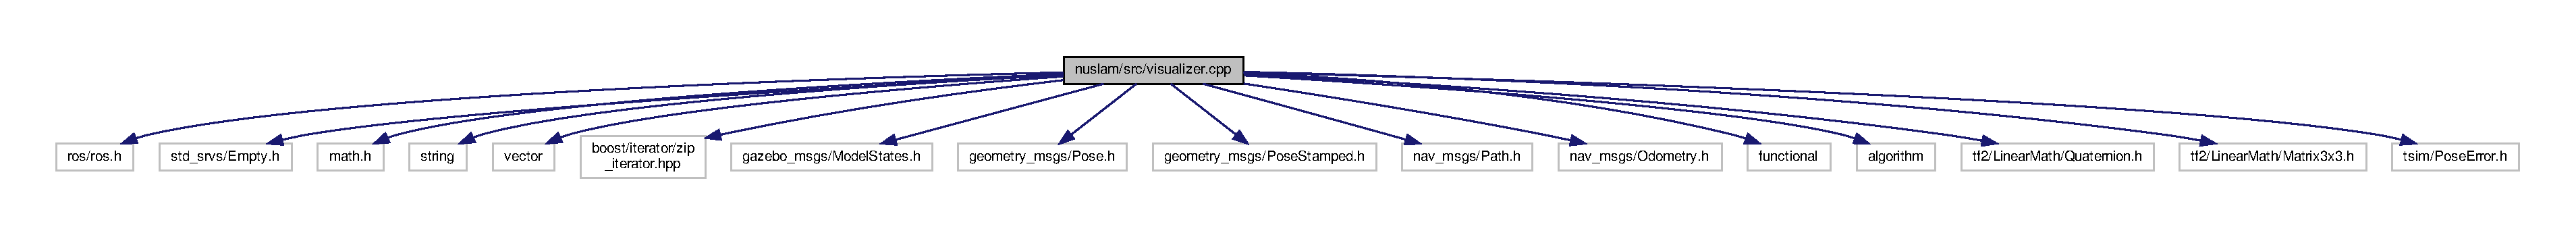
\includegraphics[width=350pt]{d1/de5/visualizer_8cpp__incl}
\end{center}
\end{figure}
\subsection*{Functions}
\begin{DoxyCompactItemize}
\item 
void \hyperlink{visualizer_8cpp_adbc02ba8fb4d3eeee5b172ca53ebf61c}{gazebo\+\_\+callback} (const gazebo\+\_\+msgs\+::\+Model\+States \&model)
\item 
void \hyperlink{visualizer_8cpp_a834848773a1eb06255ed987fa175c2fd}{odom\+\_\+callback} (const nav\+\_\+msgs\+::\+Odometry \&odom)
\item 
void \hyperlink{visualizer_8cpp_a6d0c68da38516d07a5b5ecef446a9e91}{slam\+\_\+callback} (const nav\+\_\+msgs\+::\+Odometry \&slam)
\item 
\mbox{\Hypertarget{visualizer_8cpp_a3c04138a5bfe5d72780bb7e82a18e627}\label{visualizer_8cpp_a3c04138a5bfe5d72780bb7e82a18e627}} 
int \hyperlink{visualizer_8cpp_a3c04138a5bfe5d72780bb7e82a18e627}{main} (int argc, char $\ast$$\ast$argv)
\begin{DoxyCompactList}\small\item\em The Main Function ///. \end{DoxyCompactList}\end{DoxyCompactItemize}
\subsection*{Variables}
\begin{DoxyCompactItemize}
\item 
\mbox{\Hypertarget{visualizer_8cpp_a8c7fd303c6f4941962c2ce0d0d7b01ca}\label{visualizer_8cpp_a8c7fd303c6f4941962c2ce0d0d7b01ca}} 
bool {\bfseries gazebo\+\_\+callback\+\_\+flag} = false
\item 
\mbox{\Hypertarget{visualizer_8cpp_ae812a1a12bd845b002bccc6f1e4b1d40}\label{visualizer_8cpp_ae812a1a12bd845b002bccc6f1e4b1d40}} 
bool {\bfseries odom\+\_\+callback\+\_\+flag} = false
\item 
\mbox{\Hypertarget{visualizer_8cpp_a8c94858359289e74cde99c0ca67fb47d}\label{visualizer_8cpp_a8c94858359289e74cde99c0ca67fb47d}} 
bool {\bfseries slam\+\_\+callback\+\_\+flag} = false
\item 
\mbox{\Hypertarget{visualizer_8cpp_ad5317fdaa1ce3c685ef2c6fb7d8b3a70}\label{visualizer_8cpp_ad5317fdaa1ce3c685ef2c6fb7d8b3a70}} 
std\+::vector$<$ geometry\+\_\+msgs\+::\+Pose\+Stamped $>$ {\bfseries gazebo\+\_\+poses}
\item 
\mbox{\Hypertarget{visualizer_8cpp_a72f240728be93041c5d5d63dbdcbae5a}\label{visualizer_8cpp_a72f240728be93041c5d5d63dbdcbae5a}} 
std\+::vector$<$ geometry\+\_\+msgs\+::\+Pose\+Stamped $>$ {\bfseries odom\+\_\+poses}
\item 
\mbox{\Hypertarget{visualizer_8cpp_a9727b4624cc3385d6397ff22951a58ba}\label{visualizer_8cpp_a9727b4624cc3385d6397ff22951a58ba}} 
std\+::vector$<$ geometry\+\_\+msgs\+::\+Pose\+Stamped $>$ {\bfseries slam\+\_\+poses}
\item 
\mbox{\Hypertarget{visualizer_8cpp_a30944405237aa5def944fbfd607393de}\label{visualizer_8cpp_a30944405237aa5def944fbfd607393de}} 
std\+::string {\bfseries frame\+\_\+id\+\_\+} = \char`\"{}map\char`\"{}
\end{DoxyCompactItemize}


\subsection{Detailed Description}
Publishes aggregate robot paths based on pure odometry, ground truth (Gazebo data) or the S\+L\+AM estimate. Also publishes tsim\+::\+Pose\+Error message to display error in x,y,theta between odometry and ground truth, as well as S\+L\+AM and ground truth. 

P\+A\+R\+A\+M\+E\+T\+E\+RS\+: gazebo\+\_\+callback\+\_\+flag (bool)\+: specifies whether to publish robot path from gazebo based on callback trigger odom\+\_\+callback\+\_\+flag (bool)\+: specifies whether to publish robot path from odometry based on callback trigger slam\+\_\+callback\+\_\+flag (bool)\+: specifies whether to publish robot path from S\+L\+AM estimate based on callback trigger gazebo\+\_\+poses (std\+::vector$<$geometry\+\_\+msgs\+::\+Pose\+Stamped$>$)\+: vector containing Pose\+Stamped messages for Path generation odom\+\_\+poses (std\+::vector$<$geometry\+\_\+msgs\+::\+Pose\+Stamped$>$)\+: vector containing Pose\+Stamped messages for Path generation slam\+\_\+poses (std\+::vector$<$geometry\+\_\+msgs\+::\+Pose\+Stamped$>$)\+: vector containing Pose\+Stamped messages for Path generation frame\+\_\+id\+\_\+ (string)\+: frame with respect to which path is published (\char`\"{}map\char`\"{} is the static frame in this implementation) frequency (double)\+: frequency of control loop.

P\+U\+B\+L\+I\+S\+H\+ES\+: gazebo\+\_\+path (nav\+\_\+msgs\+::\+Path)\+: publishes Path based on gazebo pose readings odom\+\_\+path (nav\+\_\+msgs\+::\+Path)\+: publishes Path based on odometry pose estimate slam\+\_\+path (nav\+\_\+msgs\+::\+Path)\+: publishes Path based on S\+L\+AM pose estimate odom\+\_\+err (tsim\+::\+Pose\+Error)\+: publishes error between odometry estimate and gazebo pose readings slam\+\_\+err (tsim\+::\+Pose\+Error)\+: publishes error between S\+L\+AM estimate and gazebo pose readings

S\+U\+B\+S\+C\+R\+I\+B\+ES\+: /gazebo/model\+\_\+states (gazebo\+\_\+msgs\+::\+Model\+States) to read robot Pose from gazebo estimate /odom (nav\+\_\+msgs\+::\+Odometry) to read robot pose from odometry estimate /slam/odom (nav\+\_\+msgs\+::\+Odometry) to read robot pose from S\+L\+AM estimate

F\+U\+N\+C\+T\+I\+O\+NS\+: gazebo\+\_\+callback (void)\+: callback for /gazebo/model\+\_\+states subscriber which appends the current pose to recorded pose history odom\+\_\+callback (void)\+: callback for /odom subscriber which appends the current pose to recorded pose history slam\+\_\+callback (void)\+: callback for /slam/odom subscriber which appends the current pose to recorded pose history 

\subsection{Function Documentation}
\mbox{\Hypertarget{visualizer_8cpp_adbc02ba8fb4d3eeee5b172ca53ebf61c}\label{visualizer_8cpp_adbc02ba8fb4d3eeee5b172ca53ebf61c}} 
\index{visualizer.\+cpp@{visualizer.\+cpp}!gazebo\+\_\+callback@{gazebo\+\_\+callback}}
\index{gazebo\+\_\+callback@{gazebo\+\_\+callback}!visualizer.\+cpp@{visualizer.\+cpp}}
\subsubsection{\texorpdfstring{gazebo\+\_\+callback()}{gazebo\_callback()}}
{\footnotesize\ttfamily void gazebo\+\_\+callback (\begin{DoxyParamCaption}\item[{const gazebo\+\_\+msgs\+::\+Model\+States \&}]{model }\end{DoxyParamCaption})}

extract turtlebot pose from Model\+States 
\begin{DoxyParams}{Parameters}
{\em gazebo\+\_\+msgs\+::\+Model\+States,containing} & the pose of all models in the environment \\
\hline
\end{DoxyParams}
\mbox{\Hypertarget{visualizer_8cpp_a834848773a1eb06255ed987fa175c2fd}\label{visualizer_8cpp_a834848773a1eb06255ed987fa175c2fd}} 
\index{visualizer.\+cpp@{visualizer.\+cpp}!odom\+\_\+callback@{odom\+\_\+callback}}
\index{odom\+\_\+callback@{odom\+\_\+callback}!visualizer.\+cpp@{visualizer.\+cpp}}
\subsubsection{\texorpdfstring{odom\+\_\+callback()}{odom\_callback()}}
{\footnotesize\ttfamily void odom\+\_\+callback (\begin{DoxyParamCaption}\item[{const nav\+\_\+msgs\+::\+Odometry \&}]{odom }\end{DoxyParamCaption})}

extract turtlebot pose from Odometry msg 
\begin{DoxyParams}{Parameters}
{\em nav\+\_\+msgs\+::\+Odometry,containing} & the robot pose \\
\hline
\end{DoxyParams}
\mbox{\Hypertarget{visualizer_8cpp_a6d0c68da38516d07a5b5ecef446a9e91}\label{visualizer_8cpp_a6d0c68da38516d07a5b5ecef446a9e91}} 
\index{visualizer.\+cpp@{visualizer.\+cpp}!slam\+\_\+callback@{slam\+\_\+callback}}
\index{slam\+\_\+callback@{slam\+\_\+callback}!visualizer.\+cpp@{visualizer.\+cpp}}
\subsubsection{\texorpdfstring{slam\+\_\+callback()}{slam\_callback()}}
{\footnotesize\ttfamily void slam\+\_\+callback (\begin{DoxyParamCaption}\item[{const nav\+\_\+msgs\+::\+Odometry \&}]{slam }\end{DoxyParamCaption})}

extract turtlebot pose from Odometry msg 
\begin{DoxyParams}{Parameters}
{\em nav\+\_\+msgs\+::\+Odometry,containing} & the robot pose \\
\hline
\end{DoxyParams}

\hypertarget{real__waypoint_8cpp}{}\section{nuturtle\+\_\+robot/src/real\+\_\+waypoint.cpp File Reference}
\label{real__waypoint_8cpp}\index{nuturtle\+\_\+robot/src/real\+\_\+waypoint.\+cpp@{nuturtle\+\_\+robot/src/real\+\_\+waypoint.\+cpp}}


Makes the turtlebot3 follow a series of waypoints using closed-\/loop odometer-\/based feedback control.  


{\ttfamily \#include $<$ros/ros.\+h$>$}\newline
{\ttfamily \#include $<$std\+\_\+srvs/\+Empty.\+h$>$}\newline
{\ttfamily \#include $<$nav\+\_\+msgs/\+Odometry.\+h$>$}\newline
{\ttfamily \#include \char`\"{}rigid2d/\+Set\+Pose.\+h\char`\"{}}\newline
{\ttfamily \#include $<$tf2/\+Linear\+Math/\+Quaternion.\+h$>$}\newline
{\ttfamily \#include $<$tf2/\+Linear\+Math/\+Matrix3x3.\+h$>$}\newline
{\ttfamily \#include $<$visualization\+\_\+msgs/\+Marker.\+h$>$}\newline
{\ttfamily \#include $<$math.\+h$>$}\newline
{\ttfamily \#include $<$string$>$}\newline
{\ttfamily \#include $<$vector$>$}\newline
{\ttfamily \#include $<$boost/iterator/zip\+\_\+iterator.\+hpp$>$}\newline
{\ttfamily \#include \char`\"{}rigid2d/waypoints.\+hpp\char`\"{}}\newline
Include dependency graph for real\+\_\+waypoint.\+cpp\+:
\nopagebreak
\begin{figure}[H]
\begin{center}
\leavevmode
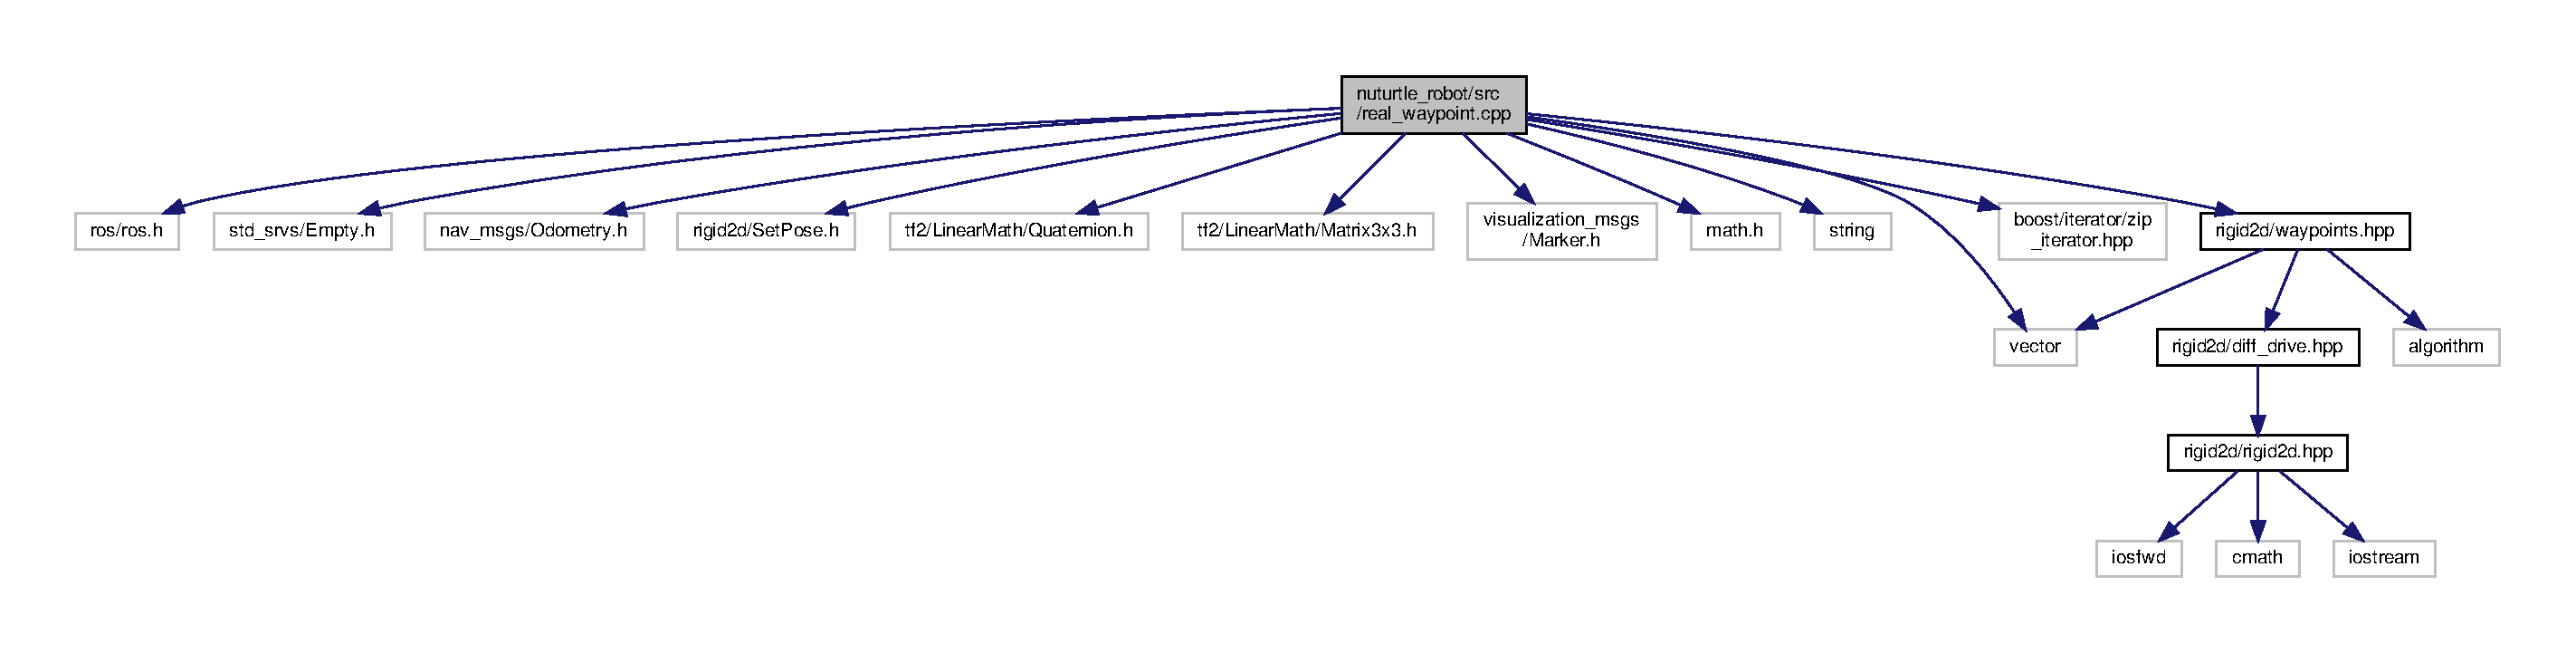
\includegraphics[width=350pt]{da/d22/real__waypoint_8cpp__incl}
\end{center}
\end{figure}
\subsection*{Functions}
\begin{DoxyCompactItemize}
\item 
void \hyperlink{real__waypoint_8cpp_ac23f42e23b70b13ce3255b21f487a507}{odom\+Callback} (const nav\+\_\+msgs\+::\+Odometry \&odom)
\item 
bool \hyperlink{real__waypoint_8cpp_aafcd8ac962841fac7d63c81baaf9369d}{start\+Callback} (std\+\_\+srvs\+::\+Empty\+::\+Request \&, std\+\_\+srvs\+::\+Empty\+::\+Response \&)
\item 
bool \hyperlink{real__waypoint_8cpp_af42b5fe5657dfc7828d0445ef89e988d}{stop\+Callback} (std\+\_\+srvs\+::\+Empty\+::\+Request \&, std\+\_\+srvs\+::\+Empty\+::\+Response \&)
\item 
\mbox{\Hypertarget{real__waypoint_8cpp_a3c04138a5bfe5d72780bb7e82a18e627}\label{real__waypoint_8cpp_a3c04138a5bfe5d72780bb7e82a18e627}} 
int \hyperlink{real__waypoint_8cpp_a3c04138a5bfe5d72780bb7e82a18e627}{main} (int argc, char $\ast$$\ast$argv)
\begin{DoxyCompactList}\small\item\em The Main Function ///. \end{DoxyCompactList}\end{DoxyCompactItemize}
\subsection*{Variables}
\begin{DoxyCompactItemize}
\item 
\mbox{\Hypertarget{real__waypoint_8cpp_a400d04156bbf7d9a5b3a3bc361d785d8}\label{real__waypoint_8cpp_a400d04156bbf7d9a5b3a3bc361d785d8}} 
\hyperlink{structrigid2d_1_1Pose2D}{rigid2d\+::\+Pose2D} {\bfseries pose}
\item 
\mbox{\Hypertarget{real__waypoint_8cpp_a44992affb21ddb63e4e7f0cc0090aca3}\label{real__waypoint_8cpp_a44992affb21ddb63e4e7f0cc0090aca3}} 
bool {\bfseries move} = false
\item 
\mbox{\Hypertarget{real__waypoint_8cpp_a3ee0ad2c2fb892e39c44a42e14f18ce4}\label{real__waypoint_8cpp_a3ee0ad2c2fb892e39c44a42e14f18ce4}} 
bool {\bfseries callback\+\_\+flag} = false
\end{DoxyCompactItemize}


\subsection{Detailed Description}
Makes the turtlebot3 follow a series of waypoints using closed-\/loop odometer-\/based feedback control. 

P\+A\+R\+A\+M\+E\+T\+E\+RS\+: waypoint\+\_\+x (vector$<$float$>$)\+: x-\/coordinates of the waypoints to visit waypoint\+\_\+y (vector$<$float$>$)\+: y-\/coordinates of the waypoints to visit frequency (int)\+: frequency of control loop. threshold (float)\+: specifies when the target pose has been reached. v\+\_\+x\+\_\+max\+\_\+ (float)\+: turtlebot3\textquotesingle{}s maximum linear velocity w\+\_\+z\+\_\+max\+\_\+ (float)\+: turtlebot3\textquotesingle{}s maximum rotational velocity frac\+\_\+vel (float)\+: fraction to be used of the turtlebot3\textquotesingle{}s maximum linear and angular velocities

pose (\hyperlink{structrigid2d_1_1Pose2D}{rigid2d\+::\+Pose2D})\+: modeled diff drive robot pose based on feedforward prediction move (bool)\+: flag to allow or prevent the publishing of Twists to cmd\+\_\+vel callback\+\_\+flag (bool)\+: flag to indicate that odometry message has been received tw (Twist)\+: used to publish linear and angular velocities to turtle1/cmd\+\_\+vel.

Vb (\hyperlink{classrigid2d_1_1Twist2D}{rigid2d\+::\+Twist2D})\+: calculated twist necessary for robot to reach current waypoint waypoints\+\_\+ (vector$<$rigid2d\+::\+Vector2\+D$>$)\+: intermediate storage of waypoints combined using waypoint\+\_\+x and y waypoints (\hyperlink{classrigid2d_1_1Waypoints}{rigid2d\+::\+Waypoints})\+: stores waypoints to visit and returns \hyperlink{classrigid2d_1_1Twist2D}{rigid2d\+::\+Twist2D} required to do so

marker (visualization\+\_\+msgs\+::\+Marker)\+: marker displayed in R\+Viz, which localizes waypoints on grid. started\+\_\+cycle (bool)\+:indicates whether new cycle has started.

P\+U\+B\+L\+I\+S\+H\+ES\+: cmd\+\_\+vel (geometry\+\_\+msgs\+::\+Twist)\+: publishes a twist with linear (x) and angular (z) velocities to command turtlebot3 visualization\+\_\+marker (visualization\+\_\+msgs\+::\+Marker)\+: publishes marker to R\+Viz to localize watpoints on grid S\+U\+B\+S\+C\+R\+I\+B\+ES\+: odom (nav\+\_\+msgs\+::\+Odometry)\+: feceives the position and orientation of the turtlebot3

F\+U\+N\+C\+T\+I\+O\+NS\+: odom\+Callback (void)\+: callback for odom subscriber, which records the turtle\textquotesingle{}s pose for use elsewhere. Also sets callback flag. start\+Callback (bool)\+: start service callback, sets move boolean to true to allow publishing of cmd\+\_\+vel stop\+Callback (bool)\+: stop service callback, sets move boolean to false to prevent publishing of cmd\+\_\+vel S\+E\+R\+V\+I\+C\+ES\+: start\+: sets move boolean to true to allow publishing of cmd\+\_\+vel stop\+: sets move boolean to false to prevent publishing of cmd\+\_\+vel 

\subsection{Function Documentation}
\mbox{\Hypertarget{real__waypoint_8cpp_ac23f42e23b70b13ce3255b21f487a507}\label{real__waypoint_8cpp_ac23f42e23b70b13ce3255b21f487a507}} 
\index{real\+\_\+waypoint.\+cpp@{real\+\_\+waypoint.\+cpp}!odom\+Callback@{odom\+Callback}}
\index{odom\+Callback@{odom\+Callback}!real\+\_\+waypoint.\+cpp@{real\+\_\+waypoint.\+cpp}}
\subsubsection{\texorpdfstring{odom\+Callback()}{odomCallback()}}
{\footnotesize\ttfamily void odom\+Callback (\begin{DoxyParamCaption}\item[{const nav\+\_\+msgs\+::\+Odometry \&}]{odom }\end{DoxyParamCaption})}

odom subscriber callback. Records turtlebot3 pose (x, y, theta)


\begin{DoxyParams}{Parameters}
{\em odom} & (nav\+\_\+msgs\+::\+Odometry) \\
\hline
\end{DoxyParams}
\begin{DoxyReturn}{Returns}
pose (\hyperlink{structrigid2d_1_1Pose2D}{rigid2d\+::\+Pose2D}) 
\end{DoxyReturn}
\mbox{\Hypertarget{real__waypoint_8cpp_aafcd8ac962841fac7d63c81baaf9369d}\label{real__waypoint_8cpp_aafcd8ac962841fac7d63c81baaf9369d}} 
\index{real\+\_\+waypoint.\+cpp@{real\+\_\+waypoint.\+cpp}!start\+Callback@{start\+Callback}}
\index{start\+Callback@{start\+Callback}!real\+\_\+waypoint.\+cpp@{real\+\_\+waypoint.\+cpp}}
\subsubsection{\texorpdfstring{start\+Callback()}{startCallback()}}
{\footnotesize\ttfamily bool start\+Callback (\begin{DoxyParamCaption}\item[{std\+\_\+srvs\+::\+Empty\+::\+Request \&}]{,  }\item[{std\+\_\+srvs\+::\+Empty\+::\+Response \&}]{ }\end{DoxyParamCaption})}

start service callback, sets move boolean to true to allow publishing of cmd\+\_\+vel \begin{DoxyReturn}{Returns}
sets move (bool) to true 
\end{DoxyReturn}
\mbox{\Hypertarget{real__waypoint_8cpp_af42b5fe5657dfc7828d0445ef89e988d}\label{real__waypoint_8cpp_af42b5fe5657dfc7828d0445ef89e988d}} 
\index{real\+\_\+waypoint.\+cpp@{real\+\_\+waypoint.\+cpp}!stop\+Callback@{stop\+Callback}}
\index{stop\+Callback@{stop\+Callback}!real\+\_\+waypoint.\+cpp@{real\+\_\+waypoint.\+cpp}}
\subsubsection{\texorpdfstring{stop\+Callback()}{stopCallback()}}
{\footnotesize\ttfamily bool stop\+Callback (\begin{DoxyParamCaption}\item[{std\+\_\+srvs\+::\+Empty\+::\+Request \&}]{,  }\item[{std\+\_\+srvs\+::\+Empty\+::\+Response \&}]{ }\end{DoxyParamCaption})}

stop service callback, sets move boolean to false to prevent publishing of cmd\+\_\+vel \begin{DoxyReturn}{Returns}
sets move (bool) to false 
\end{DoxyReturn}

\hypertarget{rotation_8cpp}{}\section{nuturtle\+\_\+robot/src/rotation.cpp File Reference}
\label{rotation_8cpp}\index{nuturtle\+\_\+robot/src/rotation.\+cpp@{nuturtle\+\_\+robot/src/rotation.\+cpp}}


Provides a /start service which makes the turtlebot3 perform either 20 rotation (C\+W/\+C\+CW) or a 2-\/meter traversal (F\+W\+D/\+B\+WD)  


{\ttfamily \#include $<$ros/ros.\+h$>$}\newline
{\ttfamily \#include $<$geometry\+\_\+msgs/\+Twist.\+h$>$}\newline
{\ttfamily \#include $<$sensor\+\_\+msgs/\+Joint\+State.\+h$>$}\newline
{\ttfamily \#include $<$string$>$}\newline
{\ttfamily \#include \char`\"{}rigid2d/rigid2d.\+hpp\char`\"{}}\newline
{\ttfamily \#include \char`\"{}rigid2d/diff\+\_\+drive.\+hpp\char`\"{}}\newline
{\ttfamily \#include \char`\"{}nuturtlebot/\+Wheel\+Commands.\+h\char`\"{}}\newline
{\ttfamily \#include \char`\"{}nuturtlebot/\+Sensor\+Data.\+h\char`\"{}}\newline
{\ttfamily \#include \char`\"{}nuturtle\+\_\+robot/\+Rotation.\+h\char`\"{}}\newline
{\ttfamily \#include \char`\"{}rigid2d/\+Set\+Pose.\+h\char`\"{}}\newline
{\ttfamily \#include $<$functional$>$}\newline
Include dependency graph for rotation.\+cpp\+:\nopagebreak
\begin{figure}[H]
\begin{center}
\leavevmode
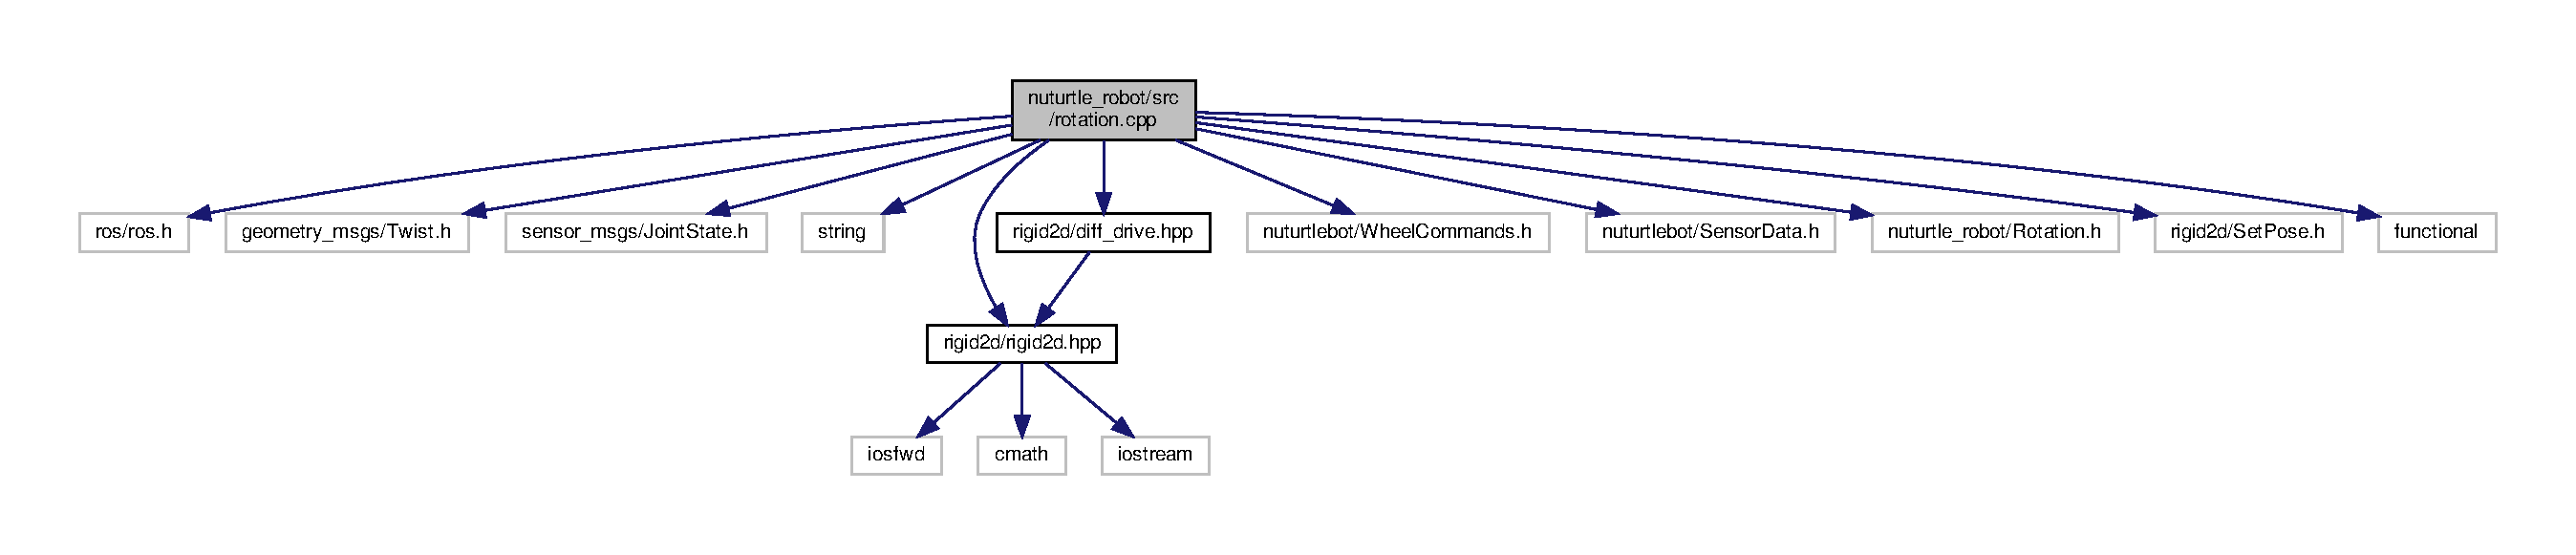
\includegraphics[width=350pt]{dc/df1/rotation_8cpp__incl}
\end{center}
\end{figure}
\subsection*{Functions}
\begin{DoxyCompactItemize}
\item 
bool \hyperlink{rotation_8cpp_a31ebe0e5041f663b63d48a54ec05494b}{start\+Callback} (nuturtle\+\_\+robot\+::\+Rotation\+::\+Request \&req, nuturtle\+\_\+robot\+::\+Rotation\+::\+Response \&res)
\item 
void \hyperlink{rotation_8cpp_aa3e1206390821164a4b362e7c55f2648}{timer\+Callback} (const ros\+::\+Timer\+Event \&, const ros\+::\+Publisher \&vel\+\_\+pub)
\item 
\mbox{\Hypertarget{rotation_8cpp_a3c04138a5bfe5d72780bb7e82a18e627}\label{rotation_8cpp_a3c04138a5bfe5d72780bb7e82a18e627}} 
int \hyperlink{rotation_8cpp_a3c04138a5bfe5d72780bb7e82a18e627}{main} (int argc, char $\ast$$\ast$argv)
\begin{DoxyCompactList}\small\item\em The Main Function ///. \end{DoxyCompactList}\end{DoxyCompactItemize}
\subsection*{Variables}
\begin{DoxyCompactItemize}
\item 
\mbox{\Hypertarget{rotation_8cpp_abf71dd72073c6c40ee2c364e567ae08c}\label{rotation_8cpp_abf71dd72073c6c40ee2c364e567ae08c}} 
nuturtle\+\_\+robot\+::\+Rotation\+::\+Request {\bfseries request}
\item 
\mbox{\Hypertarget{rotation_8cpp_a6e7901ce8d657fd6ac8c86e5e2500d25}\label{rotation_8cpp_a6e7901ce8d657fd6ac8c86e5e2500d25}} 
bool {\bfseries start\+\_\+called} = false
\item 
\mbox{\Hypertarget{rotation_8cpp_a6e85223fcd11d3cf3a1fff5b211332de}\label{rotation_8cpp_a6e85223fcd11d3cf3a1fff5b211332de}} 
int {\bfseries timer\+\_\+count} = 0
\item 
\mbox{\Hypertarget{rotation_8cpp_ab8429d3251f67d8ee440068406c90b82}\label{rotation_8cpp_ab8429d3251f67d8ee440068406c90b82}} 
bool {\bfseries cycle\+\_\+trigger} = false
\item 
\mbox{\Hypertarget{rotation_8cpp_a8c443db840e4be46a5d58abac0b85916}\label{rotation_8cpp_a8c443db840e4be46a5d58abac0b85916}} 
int {\bfseries rotation\+\_\+count} = 0
\item 
\mbox{\Hypertarget{rotation_8cpp_a5b4563ede08683c61879f1c679b11d88}\label{rotation_8cpp_a5b4563ede08683c61879f1c679b11d88}} 
int {\bfseries translation\+\_\+count} = 0
\item 
\mbox{\Hypertarget{rotation_8cpp_ad3f1aee58b6621b91b33841387188560}\label{rotation_8cpp_ad3f1aee58b6621b91b33841387188560}} 
int {\bfseries pause\+\_\+count} = 0
\item 
\mbox{\Hypertarget{rotation_8cpp_a485d7b3a5c34aa635315b70d16219ed8}\label{rotation_8cpp_a485d7b3a5c34aa635315b70d16219ed8}} 
int {\bfseries full\+\_\+rots} = 10000000
\item 
\mbox{\Hypertarget{rotation_8cpp_af7098fe636af27fcc90ed5ee1085fdb4}\label{rotation_8cpp_af7098fe636af27fcc90ed5ee1085fdb4}} 
int {\bfseries full\+\_\+trans} = 1000000
\item 
\mbox{\Hypertarget{rotation_8cpp_a5d694246db39ec0d20b46da16d6827f7}\label{rotation_8cpp_a5d694246db39ec0d20b46da16d6827f7}} 
float {\bfseries rot} = 0
\item 
\mbox{\Hypertarget{rotation_8cpp_ad618458d9c15ada2b6727db8e5a7cea5}\label{rotation_8cpp_ad618458d9c15ada2b6727db8e5a7cea5}} 
float {\bfseries trans} = 0
\end{DoxyCompactItemize}


\subsection{Detailed Description}
Provides a /start service which makes the turtlebot3 perform either 20 rotation (C\+W/\+C\+CW) or a 2-\/meter traversal (F\+W\+D/\+B\+WD) 

P\+A\+R\+A\+M\+E\+T\+E\+RS\+: request (nuturtle\+\_\+robot\+::\+Rotation\+::\+Request)\+: service request for /start service, which contains four booleans\+: rot\+\_\+trans, rot\+\_\+direction, trans\+\_\+direction start\+\_\+called (bool)\+: flag to indicate that service has been called, and rotation/translation sequence can commence. timer\+\_\+count (int)\+: keeps track of iterations required to perform one rotation or translation segment. cycle\+\_\+trigger (bool)\+: flag used to alternate between pause and actuation of turtlebot3 rotation\+\_\+count (int)\+: records the number of rotations completed since the start of the service call translation\+\_\+count (int)\+: records the number of translation completed since the start of the service call pause\+\_\+count (bool)\+: keeps track of iterations required to pause for the correct amount of time based on loop rate full\+\_\+rots (int)\+: value greater than maximum number of rotations, used for loop logic full\+\_\+trans (int)\+: value greater than maximum number of translations, used for loop logic

rot (float)\+: angular component of desired 2D twist trans (float)\+: linear component of desired 2D twist frac\+\_\+vel (float)\+: fraction to be used of the turtlebot3\textquotesingle{}s maximum linear and angular velocities max\+\_\+lin\+\_\+vel\+\_\+ (float)\+: turtlebot3\textquotesingle{}s maximum linear velocity max\+\_\+ang\+\_\+vel\+\_\+ (float)\+: turtlebot3\textquotesingle{}s maximum rotational velocity frequency (float)\+: loop rate for this operation

P\+U\+B\+L\+I\+S\+H\+ES\+: publishes Twist to cmd\+\_\+vel

F\+U\+N\+C\+T\+I\+O\+NS\+: start\+\_\+callback (bool)\+: callback for start service, which calls the set\+\_\+pose and fake/set\+\_\+pose services, then sets the appripriate flags to begin movement timer\+Callback (void)\+: deterministically publishes Twist message based on desired commands according to loop logic

S\+E\+R\+V\+I\+C\+ES\+: start\+: calls set\+\_\+pose service and intiates either 20 rotations, or a 2 meter traversal 

\subsection{Function Documentation}
\mbox{\Hypertarget{rotation_8cpp_a31ebe0e5041f663b63d48a54ec05494b}\label{rotation_8cpp_a31ebe0e5041f663b63d48a54ec05494b}} 
\index{rotation.\+cpp@{rotation.\+cpp}!start\+Callback@{start\+Callback}}
\index{start\+Callback@{start\+Callback}!rotation.\+cpp@{rotation.\+cpp}}
\subsubsection{\texorpdfstring{start\+Callback()}{startCallback()}}
{\footnotesize\ttfamily bool start\+Callback (\begin{DoxyParamCaption}\item[{nuturtle\+\_\+robot\+::\+Rotation\+::\+Request \&}]{req,  }\item[{nuturtle\+\_\+robot\+::\+Rotation\+::\+Response \&}]{res }\end{DoxyParamCaption})}

start service callback, calls set\+\_\+pose service and intiates either 20 rotations, or a 2 meter traversal 
\begin{DoxyParams}{Parameters}
{\em rot\+\_\+trans} & (bool)\+: False -\/ Rotation, True -\/ Translation \\
\hline
{\em rot\+\_\+direction} & (bool)\+: False -\/ CW, True -\/ C\+CW \\
\hline
{\em trans\+\_\+direction} & (bool)\+: False -\/ Forward, True -\/ Backwards \\
\hline
\end{DoxyParams}
\begin{DoxyReturn}{Returns}
result (bool)\+: True or False. 
\end{DoxyReturn}
\mbox{\Hypertarget{rotation_8cpp_aa3e1206390821164a4b362e7c55f2648}\label{rotation_8cpp_aa3e1206390821164a4b362e7c55f2648}} 
\index{rotation.\+cpp@{rotation.\+cpp}!timer\+Callback@{timer\+Callback}}
\index{timer\+Callback@{timer\+Callback}!rotation.\+cpp@{rotation.\+cpp}}
\subsubsection{\texorpdfstring{timer\+Callback()}{timerCallback()}}
{\footnotesize\ttfamily void timer\+Callback (\begin{DoxyParamCaption}\item[{const ros\+::\+Timer\+Event \&}]{,  }\item[{const ros\+::\+Publisher \&}]{vel\+\_\+pub }\end{DoxyParamCaption})}

deterministic timer to publish Twist messages to cmd\+\_\+vel 
\begin{DoxyParams}{Parameters}
{\em ros\+::\+Timer\+Event} & ensures loop is consistent (deterministic) \\
\hline
{\em vel\+\_\+pub} & (ros\+::\+Publisher)\+: publisher object used to send messages to cmd\+\_\+\+Vel \\
\hline
\end{DoxyParams}
\begin{DoxyReturn}{Returns}
publishes Twist to cmd\+\_\+vel 
\end{DoxyReturn}

\hypertarget{turtle__interface_8cpp}{}\section{nuturtle\+\_\+robot/src/turtle\+\_\+interface.cpp File Reference}
\label{turtle__interface_8cpp}\index{nuturtle\+\_\+robot/src/turtle\+\_\+interface.\+cpp@{nuturtle\+\_\+robot/src/turtle\+\_\+interface.\+cpp}}


This node executes low-\/level control for the turtlebot, engaging its motors depending on desired twist, and reading its wheel encoder values.  


{\ttfamily \#include $<$ros/ros.\+h$>$}\newline
{\ttfamily \#include $<$geometry\+\_\+msgs/\+Twist.\+h$>$}\newline
{\ttfamily \#include $<$sensor\+\_\+msgs/\+Joint\+State.\+h$>$}\newline
{\ttfamily \#include $<$string$>$}\newline
{\ttfamily \#include \char`\"{}rigid2d/rigid2d.\+hpp\char`\"{}}\newline
{\ttfamily \#include \char`\"{}rigid2d/diff\+\_\+drive.\+hpp\char`\"{}}\newline
{\ttfamily \#include \char`\"{}nuturtlebot/\+Wheel\+Commands.\+h\char`\"{}}\newline
{\ttfamily \#include \char`\"{}nuturtlebot/\+Sensor\+Data.\+h\char`\"{}}\newline
Include dependency graph for turtle\+\_\+interface.\+cpp\+:\nopagebreak
\begin{figure}[H]
\begin{center}
\leavevmode
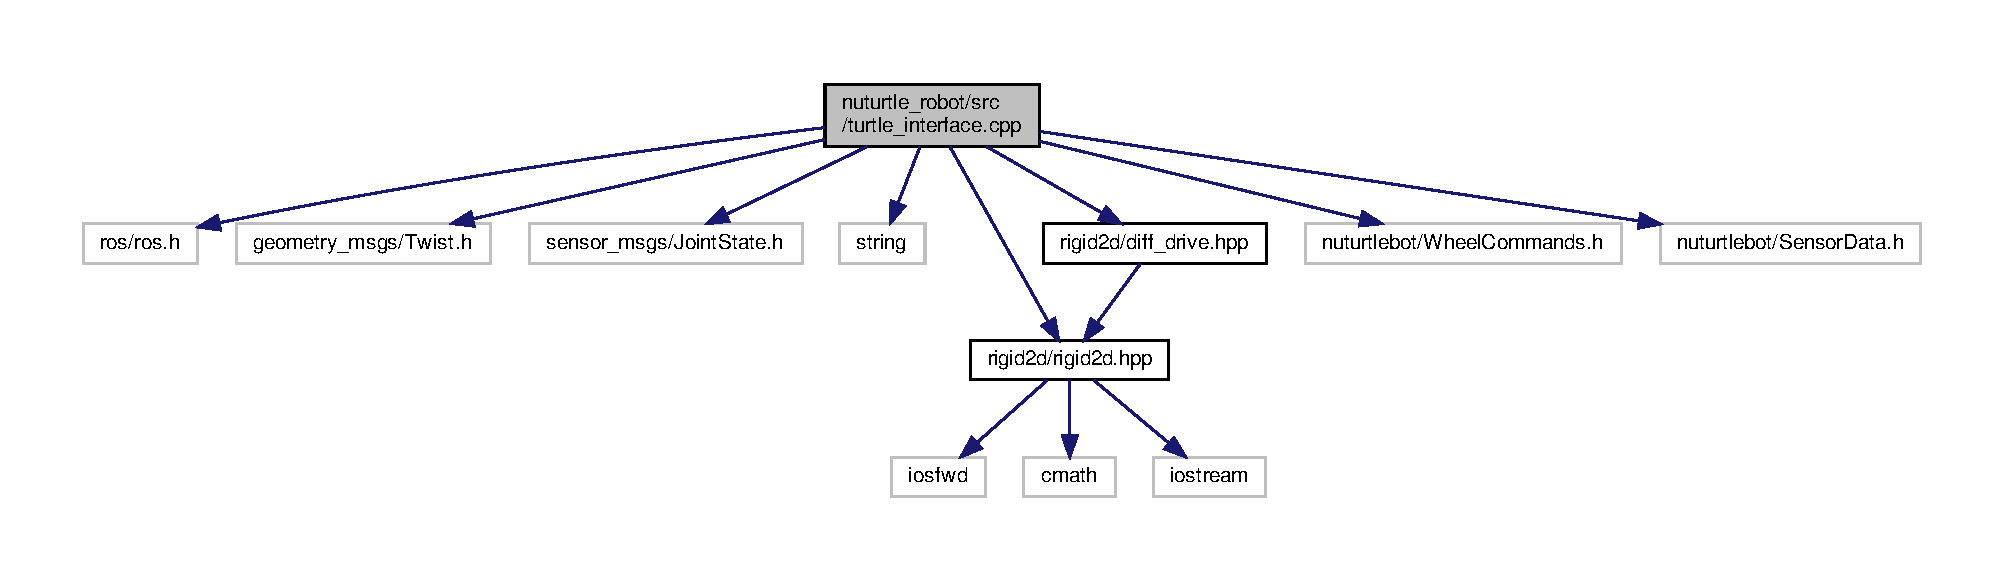
\includegraphics[width=350pt]{d5/d71/turtle__interface_8cpp__incl}
\end{center}
\end{figure}
\subsection*{Functions}
\begin{DoxyCompactItemize}
\item 
void \hyperlink{turtle__interface_8cpp_a647c2d49e90958302787373cf0bf90b7}{vel\+\_\+callback} (const geometry\+\_\+msgs\+::\+Twist \&tw)
\item 
void \hyperlink{turtle__interface_8cpp_aefea32b63b7ca4bc8c0d4d72245e3308}{sensor\+\_\+callback} (const nuturtlebot\+::\+Sensor\+Data \&sns)
\item 
\mbox{\Hypertarget{turtle__interface_8cpp_a3c04138a5bfe5d72780bb7e82a18e627}\label{turtle__interface_8cpp_a3c04138a5bfe5d72780bb7e82a18e627}} 
int \hyperlink{turtle__interface_8cpp_a3c04138a5bfe5d72780bb7e82a18e627}{main} (int argc, char $\ast$$\ast$argv)
\begin{DoxyCompactList}\small\item\em The Main Function ///. \end{DoxyCompactList}\end{DoxyCompactItemize}
\subsection*{Variables}
\begin{DoxyCompactItemize}
\item 
\mbox{\Hypertarget{turtle__interface_8cpp_a002f817728ce76d60fecd0d2b5bcd214}\label{turtle__interface_8cpp_a002f817728ce76d60fecd0d2b5bcd214}} 
\hyperlink{structrigid2d_1_1WheelVelocities}{rigid2d\+::\+Wheel\+Velocities} {\bfseries w\+\_\+vel}
\item 
\mbox{\Hypertarget{turtle__interface_8cpp_ac1f993698ce846b2cf46cc4b76f40e2f}\label{turtle__interface_8cpp_ac1f993698ce846b2cf46cc4b76f40e2f}} 
\hyperlink{structrigid2d_1_1WheelVelocities}{rigid2d\+::\+Wheel\+Velocities} {\bfseries w\+\_\+vel\+\_\+measured}
\item 
\mbox{\Hypertarget{turtle__interface_8cpp_a2e231184bf093953a82dd28fe0151cd6}\label{turtle__interface_8cpp_a2e231184bf093953a82dd28fe0151cd6}} 
\hyperlink{structrigid2d_1_1WheelVelocities}{rigid2d\+::\+Wheel\+Velocities} {\bfseries w\+\_\+ang}
\item 
\mbox{\Hypertarget{turtle__interface_8cpp_aae05b70475acb90fabcbcb02075b4a5c}\label{turtle__interface_8cpp_aae05b70475acb90fabcbcb02075b4a5c}} 
\hyperlink{classrigid2d_1_1DiffDrive}{rigid2d\+::\+Diff\+Drive} {\bfseries driver}
\item 
\mbox{\Hypertarget{turtle__interface_8cpp_a4c45cdff103e6644a620ba5061509f22}\label{turtle__interface_8cpp_a4c45cdff103e6644a620ba5061509f22}} 
double {\bfseries frequency} = 60
\item 
\mbox{\Hypertarget{turtle__interface_8cpp_a26852b023731e379cdad159adc7057a1}\label{turtle__interface_8cpp_a26852b023731e379cdad159adc7057a1}} 
bool {\bfseries vel\+\_\+flag} = false
\item 
\mbox{\Hypertarget{turtle__interface_8cpp_ad0f8f30758fdc7dce29ed6bc0c7ec022}\label{turtle__interface_8cpp_ad0f8f30758fdc7dce29ed6bc0c7ec022}} 
bool {\bfseries sensor\+\_\+flag} = false
\item 
\mbox{\Hypertarget{turtle__interface_8cpp_aa9a594746d47d94a5781f23394dc6552}\label{turtle__interface_8cpp_aa9a594746d47d94a5781f23394dc6552}} 
float {\bfseries max\+\_\+lin\+\_\+vel\+\_\+} = 0
\item 
\mbox{\Hypertarget{turtle__interface_8cpp_a1114e456737892d7ceea75bf06edb7b6}\label{turtle__interface_8cpp_a1114e456737892d7ceea75bf06edb7b6}} 
float {\bfseries max\+\_\+ang\+\_\+vel\+\_\+} = 0
\item 
\mbox{\Hypertarget{turtle__interface_8cpp_ae1f1f750988ce185081f948f43488cd2}\label{turtle__interface_8cpp_ae1f1f750988ce185081f948f43488cd2}} 
float {\bfseries motor\+\_\+rot\+\_\+max\+\_\+} = 0
\item 
\mbox{\Hypertarget{turtle__interface_8cpp_a4a7181cc1f73825c5452e0310f73d2a2}\label{turtle__interface_8cpp_a4a7181cc1f73825c5452e0310f73d2a2}} 
float {\bfseries encoder\+\_\+ticks\+\_\+per\+\_\+rev\+\_\+} = 0
\end{DoxyCompactItemize}


\subsection{Detailed Description}
This node executes low-\/level control for the turtlebot, engaging its motors depending on desired twist, and reading its wheel encoder values. 

P\+A\+R\+A\+M\+E\+T\+E\+RS\+: w\+\_\+vel (\hyperlink{structrigid2d_1_1WheelVelocities}{rigid2d\+::\+Wheel\+Velocities})\+: used to store wheel commands, ranging from -\/265 to +265 as converted from actual wheel velocities. w\+\_\+vel\+\_\+measured (\hyperlink{structrigid2d_1_1WheelVelocities}{rigid2d\+::\+Wheel\+Velocities})\+: measured wheel velocity, computed by feeding updated wheel encoder values to Diff\+Drive\+::update\+Odomtry() w\+\_\+ang (\hyperlink{structrigid2d_1_1WheelVelocities}{rigid2d\+::\+Wheel\+Velocities})\+: used to store wheel angles after they are converted from wheel encoder values, where 0-\/4096 maps to 0-\/2.\+0$\ast$\+PI driver (\hyperlink{classrigid2d_1_1DiffDrive}{rigid2d\+::\+Diff\+Drive})\+: diff\+\_\+drive object used to perform operations to set turtlebot3 commands and interpret its data. frequency (double)\+: the loop rate vel\+\_\+flag (bool)\+: flag to indicate that vel\+\_\+callback has been triggered, and that a wheel command should be published. sensor\+\_\+flag (bool)\+: flag to indicate that sensor\+\_\+callback has been triggered, and that wheel joint states should be published max\+\_\+lin\+\_\+vel\+\_\+ (float)\+: the turtlebot\textquotesingle{}s maximum linear velocity in m/s max\+\_\+ang\+\_\+vel\+\_\+ (float)\+: the turtlebot\textquotesingle{}s maximum angular velocity in rad/s motor\+\_\+rot\+\_\+max\+\_\+ (float)\+: the turtlebot wheels\textquotesingle{} maximum rotational speed in rad/s encoder\+\_\+ticks\+\_\+per\+\_\+rev\+\_\+ (float)\+: used to map between wheel encoder ticks and actual wheel rotation. Cast as float to use in division

o\+\_\+fid\+\_\+ (std\+::string)\+: odometer frame ID b\+\_\+fid\+\_\+ (std\+::string)\+: body frame ID wl\+\_\+fid\+\_\+ (std\+::string)\+: left wheel frame ID wr\+\_\+fid\+\_\+ (std\+::string)\+: right wheel frame ID wbase\+\_\+ (float)\+: wheel base wrad\+\_\+ (float)\+: wheel radius

P\+U\+B\+L\+I\+S\+H\+ES\+: joint\+\_\+states (sensor\+\_\+msgs\+::\+Joint\+State)\+: the turtlebot3\textquotesingle{}s wheel positions and velocities wheel\+\_\+cmd (nuturtlebot\+::\+Wheel\+Commands)\+: the turtlebot3\textquotesingle{}s wheel commands; integers corresponding to wheel velocities from -\/max to max in rad/s

S\+U\+B\+S\+C\+R\+I\+B\+ES\+: cmd\+\_\+vel (geometry\+\_\+msgs\+::\+Twist)\+: subscriber, which records the commanded twist sensor\+\_\+data (nuturtlebot\+::\+Sensor\+Data)\+: subscriber, which records wheel encoder values, among other turtlebot3 sensor data

F\+U\+N\+C\+T\+I\+O\+NS\+: vel\+\_\+callback (void)\+: callback for cmd\+\_\+vel subscriber, which records the commanded twist and sets a flag to publish wheel commands sensor\+\_\+callback (void)\+: callback for sensor\+\_\+data subscriber, which records the turtlebot3\textquotesingle{}s wheel positions and sets a flag to publish joint states 

\subsection{Function Documentation}
\mbox{\Hypertarget{turtle__interface_8cpp_aefea32b63b7ca4bc8c0d4d72245e3308}\label{turtle__interface_8cpp_aefea32b63b7ca4bc8c0d4d72245e3308}} 
\index{turtle\+\_\+interface.\+cpp@{turtle\+\_\+interface.\+cpp}!sensor\+\_\+callback@{sensor\+\_\+callback}}
\index{sensor\+\_\+callback@{sensor\+\_\+callback}!turtle\+\_\+interface.\+cpp@{turtle\+\_\+interface.\+cpp}}
\subsubsection{\texorpdfstring{sensor\+\_\+callback()}{sensor\_callback()}}
{\footnotesize\ttfamily void sensor\+\_\+callback (\begin{DoxyParamCaption}\item[{const nuturtlebot\+::\+Sensor\+Data \&}]{sns }\end{DoxyParamCaption})}

sensor\+\_\+data subscriber callback. Records left and right wheel angles


\begin{DoxyParams}{Parameters}
{\em sns} & (nuturtlebot\+::\+Sensor\+Data )\+: the left and right wheel joint encoder values w\+\_\+ang and w\+\_\+vel\+\_\+measured (\hyperlink{structrigid2d_1_1WheelVelocities}{rigid2d\+::\+Wheel\+Velocities})\+: measured wheel angles and velocities respct. \\
\hline
\end{DoxyParams}
\mbox{\Hypertarget{turtle__interface_8cpp_a647c2d49e90958302787373cf0bf90b7}\label{turtle__interface_8cpp_a647c2d49e90958302787373cf0bf90b7}} 
\index{turtle\+\_\+interface.\+cpp@{turtle\+\_\+interface.\+cpp}!vel\+\_\+callback@{vel\+\_\+callback}}
\index{vel\+\_\+callback@{vel\+\_\+callback}!turtle\+\_\+interface.\+cpp@{turtle\+\_\+interface.\+cpp}}
\subsubsection{\texorpdfstring{vel\+\_\+callback()}{vel\_callback()}}
{\footnotesize\ttfamily void vel\+\_\+callback (\begin{DoxyParamCaption}\item[{const geometry\+\_\+msgs\+::\+Twist \&}]{tw }\end{DoxyParamCaption})}

cmd\+\_\+vel subscriber callback. Records commanded twist


\begin{DoxyParams}{Parameters}
{\em tw} & (geometry\+\_\+msgs\+::\+Twist)\+: the commanded linear and angular velocity \\
\hline
\end{DoxyParams}
\begin{DoxyReturn}{Returns}
w\+\_\+vel (\hyperlink{structrigid2d_1_1WheelVelocities}{rigid2d\+::\+Wheel\+Velocities} --$>$ nuturtlebot\+:Wheel\+Commands) to actuate turtlebot3
\end{DoxyReturn}
This function runs every time we get a geometry\+\_\+msgs\+::\+Twist message on the \char`\"{}cmd\+\_\+vel\char`\"{} topic. We generally use the const $<$message$>$Const\+Ptr \&msg syntax to prevent our node from accidentally changing the message, in the case that another node is also listening to it.
\hypertarget{diff__drive_8hpp}{}\section{rigid2d/include/rigid2d/diff\+\_\+drive.hpp File Reference}
\label{diff__drive_8hpp}\index{rigid2d/include/rigid2d/diff\+\_\+drive.\+hpp@{rigid2d/include/rigid2d/diff\+\_\+drive.\+hpp}}


Library Diff\+Drive robot kinematics and odometry.  


{\ttfamily \#include \char`\"{}rigid2d/rigid2d.\+hpp\char`\"{}}\newline
Include dependency graph for diff\+\_\+drive.\+hpp\+:
\nopagebreak
\begin{figure}[H]
\begin{center}
\leavevmode
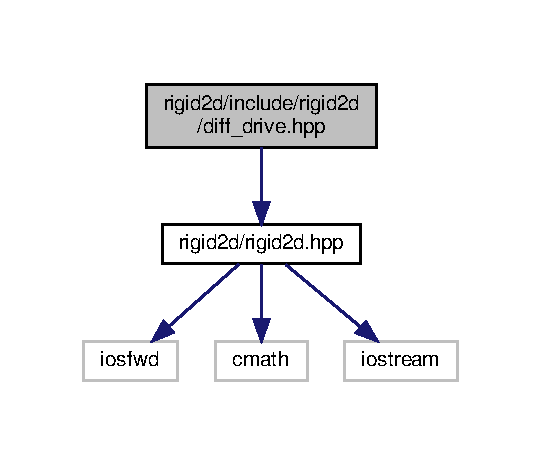
\includegraphics[width=260pt]{dd/d54/diff__drive_8hpp__incl}
\end{center}
\end{figure}
This graph shows which files directly or indirectly include this file\+:
\nopagebreak
\begin{figure}[H]
\begin{center}
\leavevmode
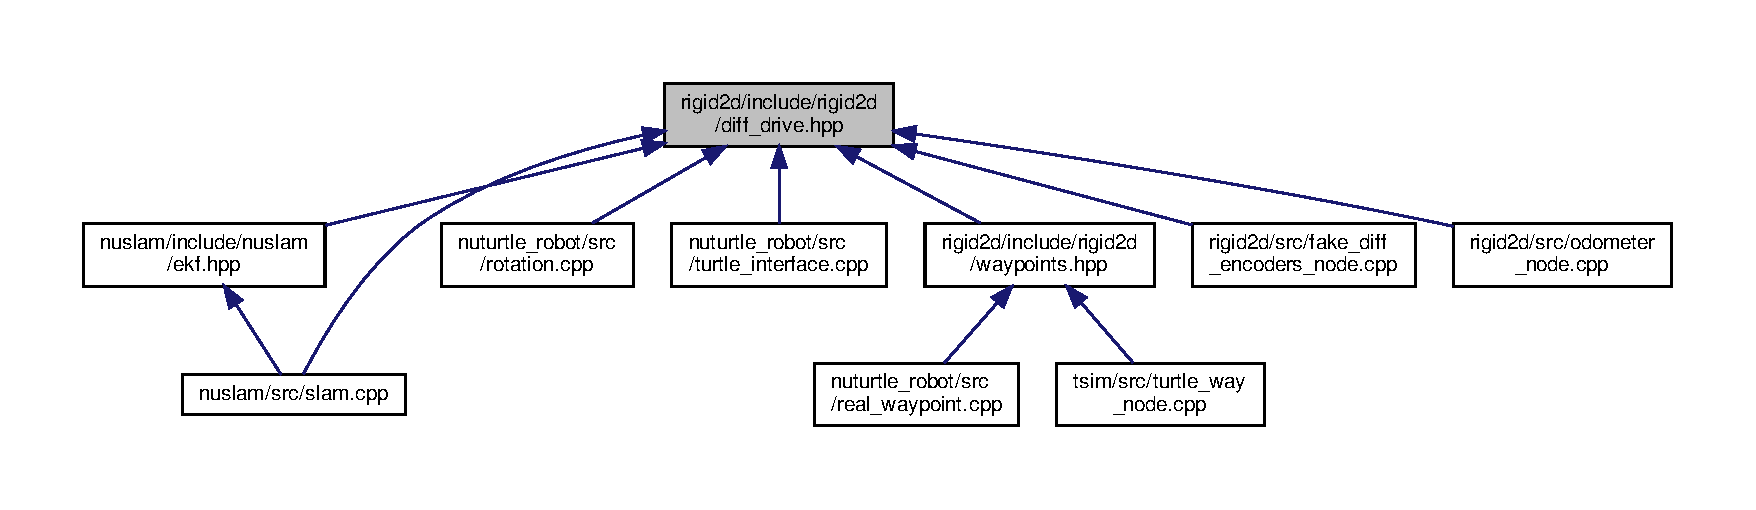
\includegraphics[width=350pt]{dc/d97/diff__drive_8hpp__dep__incl}
\end{center}
\end{figure}
\subsection*{Classes}
\begin{DoxyCompactItemize}
\item 
struct \hyperlink{structrigid2d_1_1Pose2D}{rigid2d\+::\+Pose2D}
\begin{DoxyCompactList}\small\item\em A 2-\/\+Dimensional Pose. \end{DoxyCompactList}\item 
struct \hyperlink{structrigid2d_1_1WheelVelocities}{rigid2d\+::\+Wheel\+Velocities}
\begin{DoxyCompactList}\small\item\em Wheel Velocities (rad/s) \end{DoxyCompactList}\item 
class \hyperlink{classrigid2d_1_1DiffDrive}{rigid2d\+::\+Diff\+Drive}
\begin{DoxyCompactList}\small\item\em create a \hyperlink{classrigid2d_1_1DiffDrive}{Diff\+Drive} model \end{DoxyCompactList}\end{DoxyCompactItemize}
\subsection*{Functions}
\begin{DoxyCompactItemize}
\item 
\mbox{\Hypertarget{diff__drive_8hpp_ae19b8bb4161a8164cdcedd017f0c1ef5}\label{diff__drive_8hpp_ae19b8bb4161a8164cdcedd017f0c1ef5}} 
constexpr double {\bfseries rigid2d\+::normalize\+\_\+encoders} (double rad)
\item 
std\+::ostream \& \hyperlink{diff__drive_8hpp_a7d9be2ae92a074c86f6d10807509a98a}{rigid2d\+::operator$<$$<$} (std\+::ostream \&os, const Diff\+Drive \&driver)
\begin{DoxyCompactList}\small\item\em should print a human readable version of the twist\+: An example output\+: wl\+: (rad), wr\+: (rad) \end{DoxyCompactList}\end{DoxyCompactItemize}


\subsection{Detailed Description}
Library Diff\+Drive robot kinematics and odometry. 



\subsection{Function Documentation}
\mbox{\Hypertarget{diff__drive_8hpp_file_a7d9be2ae92a074c86f6d10807509a98a}\label{diff__drive_8hpp_file_a7d9be2ae92a074c86f6d10807509a98a}} 
\index{diff\+\_\+drive.\+hpp@{diff\+\_\+drive.\+hpp}!operator$<$$<$@{operator$<$$<$}}
\index{operator$<$$<$@{operator$<$$<$}!diff\+\_\+drive.\+hpp@{diff\+\_\+drive.\+hpp}}
\subsubsection{\texorpdfstring{operator$<$$<$()}{operator<<()}}
{\footnotesize\ttfamily std\+::ostream \& rigid2d\+::operator$<$$<$ (\begin{DoxyParamCaption}\item[{std\+::ostream \&}]{os,  }\item[{const \hyperlink{classrigid2d_1_1DiffDrive}{Diff\+Drive} \&}]{driver }\end{DoxyParamCaption})}



should print a human readable version of the twist\+: An example output\+: wl\+: (rad), wr\+: (rad) 


\begin{DoxyParams}{Parameters}
{\em os} & -\/ an output stream \\
\hline
{\em dd} & -\/ the diffdrive wheel angles to print \\
\hline
\end{DoxyParams}

\hypertarget{rigid2d_8hpp}{}\section{rigid2d/include/rigid2d/rigid2d.hpp File Reference}
\label{rigid2d_8hpp}\index{rigid2d/include/rigid2d/rigid2d.\+hpp@{rigid2d/include/rigid2d/rigid2d.\+hpp}}


Library for two-\/dimensional rigid body transformations.  


{\ttfamily \#include $<$iosfwd$>$}\newline
{\ttfamily \#include $<$cmath$>$}\newline
{\ttfamily \#include $<$iostream$>$}\newline
Include dependency graph for rigid2d.\+hpp\+:\nopagebreak
\begin{figure}[H]
\begin{center}
\leavevmode
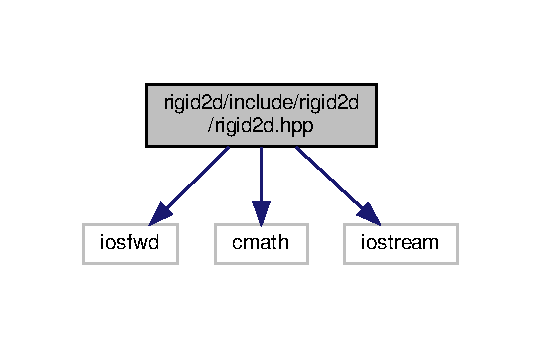
\includegraphics[width=260pt]{d9/d5e/rigid2d_8hpp__incl}
\end{center}
\end{figure}
This graph shows which files directly or indirectly include this file\+:\nopagebreak
\begin{figure}[H]
\begin{center}
\leavevmode
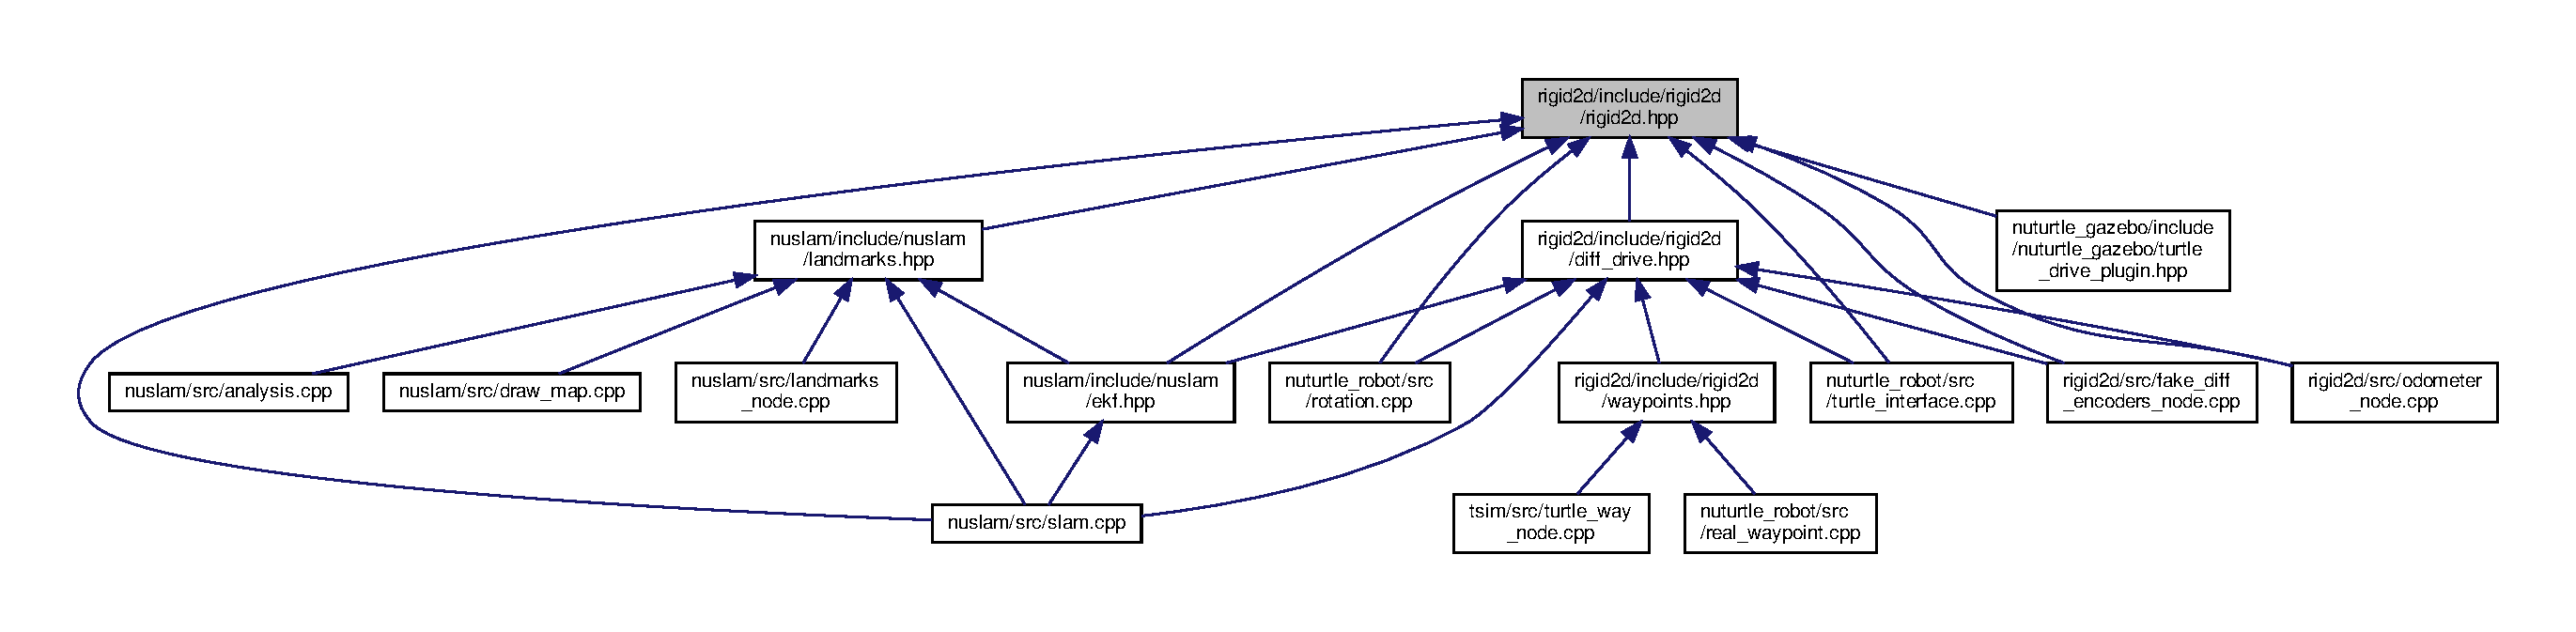
\includegraphics[width=350pt]{dc/ddb/rigid2d_8hpp__dep__incl}
\end{center}
\end{figure}
\subsection*{Classes}
\begin{DoxyCompactItemize}
\item 
struct \hyperlink{structrigid2d_1_1Vector2D}{rigid2d\+::\+Vector2D}
\begin{DoxyCompactList}\small\item\em A 2-\/\+Dimensional Vector. \end{DoxyCompactList}\item 
struct \hyperlink{structrigid2d_1_1Transform2DS}{rigid2d\+::\+Transform2\+DS}
\begin{DoxyCompactList}\small\item\em Struct version of \hyperlink{classrigid2d_1_1Transform2D}{Transform2D} to return private params. \end{DoxyCompactList}\item 
struct \hyperlink{structrigid2d_1_1Screw2D}{rigid2d\+::\+Screw2D}
\begin{DoxyCompactList}\small\item\em Screw Axis. \end{DoxyCompactList}\item 
class \hyperlink{classrigid2d_1_1Transform2D}{rigid2d\+::\+Transform2D}
\begin{DoxyCompactList}\small\item\em a rigid body transformation in 2 dimensions \end{DoxyCompactList}\item 
class \hyperlink{classrigid2d_1_1Twist2D}{rigid2d\+::\+Twist2D}
\begin{DoxyCompactList}\small\item\em a two-\/dimensional twist \end{DoxyCompactList}\end{DoxyCompactItemize}
\subsection*{Functions}
\begin{DoxyCompactItemize}
\item 
constexpr bool \hyperlink{rigid2d_8hpp_aa56fa40a409082af8395dbd4e1a25b1b}{rigid2d\+::almost\+\_\+equal} (double d1, double d2, double epsilon=1.\+0e-\/12)
\begin{DoxyCompactList}\small\item\em approximately compare two floating-\/point numbers using an absolute comparison \end{DoxyCompactList}\item 
constexpr double \hyperlink{rigid2d_8hpp_a58a218146f51c0c2454e5fe1a83cb04c}{rigid2d\+::deg2rad} (double deg)
\begin{DoxyCompactList}\small\item\em convert degrees to radians \end{DoxyCompactList}\item 
constexpr double \hyperlink{rigid2d_8hpp_a6883dbf1c0018c962e890754e9d5f62f}{rigid2d\+::rad2deg} (double rad)
\begin{DoxyCompactList}\small\item\em convert radians to degrees \end{DoxyCompactList}\item 
constexpr double \hyperlink{rigid2d_8hpp_a0366e0678d25f256b74525151b28b1e0}{rigid2d\+::normalize\+\_\+angle} (double rad)
\begin{DoxyCompactList}\small\item\em wraps an angle between +-\/ PI \end{DoxyCompactList}\item 
double \hyperlink{rigid2d_8hpp_a59fa968edf0be9b4222d18303ce2398c}{rigid2d\+::length} (const Vector2D \&v)
\begin{DoxyCompactList}\small\item\em compute the length of a \hyperlink{structrigid2d_1_1Vector2D}{Vector2D} \end{DoxyCompactList}\item 
double \hyperlink{rigid2d_8hpp_a981e57a9692ce07216b52877490f0b6f}{rigid2d\+::distance} (const Vector2D \&v1, const Vector2D \&v2)
\begin{DoxyCompactList}\small\item\em compute the distance between two Vector2\+Ds \end{DoxyCompactList}\item 
double \hyperlink{rigid2d_8hpp_ab6540af7e1f85c3892d9314653d75d9d}{rigid2d\+::angle} (const Vector2D \&v)
\begin{DoxyCompactList}\small\item\em compute the angle of a \hyperlink{structrigid2d_1_1Vector2D}{Vector2D} \end{DoxyCompactList}\item 
Vector2D \hyperlink{rigid2d_8hpp_a120e313a56ef91d46c3fed3b50674ec8}{rigid2d\+::operator+} (Vector2D lhs, const Vector2D \&rhs)
\begin{DoxyCompactList}\small\item\em perform vector addition \end{DoxyCompactList}\item 
Vector2D \hyperlink{rigid2d_8hpp_ac03d4e0cdb43893c885372b0afe358fb}{rigid2d\+::operator-\/} (Vector2D lhs, const Vector2D \&rhs)
\begin{DoxyCompactList}\small\item\em perform vector subtraction \end{DoxyCompactList}\item 
Vector2D \hyperlink{rigid2d_8hpp_affee9ba505ed1bc12215074e1b243ff5}{rigid2d\+::operator$\ast$} (Vector2D v, const double \&scalar)
\begin{DoxyCompactList}\small\item\em perform scalar multiplication on a vector from L\+HS \end{DoxyCompactList}\item 
Vector2D \hyperlink{rigid2d_8hpp_a255f1524443aead49cdf41e17a9ce443}{rigid2d\+::operator$\ast$} (const double \&scalar, Vector2D v)
\begin{DoxyCompactList}\small\item\em perform scalar multiplication on a vector from R\+HS \end{DoxyCompactList}\item 
\mbox{\Hypertarget{rigid2d_8hpp_ad6225047f92d9b508ea8169ac629a33d}\label{rigid2d_8hpp_ad6225047f92d9b508ea8169ac629a33d}} 
std\+::ostream \& \hyperlink{rigid2d_8hpp_ad6225047f92d9b508ea8169ac629a33d}{rigid2d\+::operator$<$$<$} (std\+::ostream \&os, const Vector2D \&v)
\begin{DoxyCompactList}\small\item\em output a 2 dimensional vector as \mbox{[}xcomponent ycomponent\mbox{]} os -\/ stream to output to v -\/ the vector to print \end{DoxyCompactList}\item 
\mbox{\Hypertarget{rigid2d_8hpp_a6be2725ac611fb926359452705a2a78b}\label{rigid2d_8hpp_a6be2725ac611fb926359452705a2a78b}} 
std\+::istream \& \hyperlink{rigid2d_8hpp_a6be2725ac611fb926359452705a2a78b}{rigid2d\+::operator$>$$>$} (std\+::istream \&is, Vector2D \&v)
\begin{DoxyCompactList}\small\item\em input a 2 dimensional vector You should be able to read vectors entered as two numbers separated by a newline or a space, or entered as \mbox{[}xcomponent ycomponent\mbox{]} is -\/ stream from which to read v \mbox{[}out\mbox{]} -\/ output vector Hint\+: The following may be useful\+: \href{https://en.cppreference.com/w/cpp/io/basic_istream/peek}{\tt https\+://en.\+cppreference.\+com/w/cpp/io/basic\+\_\+istream/peek} \href{https://en.cppreference.com/w/cpp/io/basic_istream/get}{\tt https\+://en.\+cppreference.\+com/w/cpp/io/basic\+\_\+istream/get} \end{DoxyCompactList}\item 
std\+::ostream \& \hyperlink{rigid2d_8hpp_aa6e4ecc06706f3e94aaebb9ba4598d30}{rigid2d\+::operator$<$$<$} (std\+::ostream \&os, const Transform2D \&tf)
\begin{DoxyCompactList}\small\item\em should print a human readable version of the transform\+: An example output\+: dtheta (degrees)\+: 90 dx\+: 3 dy\+: 5 \end{DoxyCompactList}\item 
std\+::istream \& \hyperlink{rigid2d_8hpp_aa8a4c013498f57be323a74a4a39d7355}{rigid2d\+::operator$>$$>$} (std\+::istream \&is, Transform2D \&tf)
\begin{DoxyCompactList}\small\item\em Read a transformation from stdin Should be able to read input either as output by operator$<$$<$ or as 3 numbers (degrees, dx, dy) separated by spaces or newlines. \end{DoxyCompactList}\item 
Transform2D \hyperlink{rigid2d_8hpp_a193e435d7d7f317928d3a297d4c24172}{rigid2d\+::operator$\ast$} (Transform2D lhs, const Transform2D \&rhs)
\begin{DoxyCompactList}\small\item\em multiply two transforms together, returning their composition \end{DoxyCompactList}\item 
std\+::ostream \& \hyperlink{rigid2d_8hpp_ac5c87da47bdcc94113443c120872aa2f}{rigid2d\+::operator$<$$<$} (std\+::ostream \&os, const Twist2D \&tw)
\begin{DoxyCompactList}\small\item\em should print a human readable version of the twist\+: An example output\+: dtheta (degrees)\+: 90 dx\+: 3 dy\+: 5 \end{DoxyCompactList}\item 
std\+::istream \& \hyperlink{rigid2d_8hpp_ab3dbb63aa66f6e11552fa74402b74166}{rigid2d\+::operator$>$$>$} (std\+::istream \&is, Twist2D \&tw)
\begin{DoxyCompactList}\small\item\em Read a twist from stdin Should be able to read input either as output by operator$<$$<$ or as 3 numbers (w\+\_\+z, v\+\_\+x, v\+\_\+y) separated by spaces or newlines. \end{DoxyCompactList}\end{DoxyCompactItemize}
\subsection*{Variables}
\begin{DoxyCompactItemize}
\item 
\mbox{\Hypertarget{rigid2d_8hpp_af68d2597a40a3021e2c66d1c23019952}\label{rigid2d_8hpp_af68d2597a40a3021e2c66d1c23019952}} 
constexpr double \hyperlink{rigid2d_8hpp_af68d2597a40a3021e2c66d1c23019952}{rigid2d\+::\+PI} =3.\+14159265358979323846
\begin{DoxyCompactList}\small\item\em PI. Not in C++ standard until C++20. \end{DoxyCompactList}\end{DoxyCompactItemize}


\subsection{Detailed Description}
Library for two-\/dimensional rigid body transformations. 



\subsection{Function Documentation}
\mbox{\Hypertarget{rigid2d_8hpp_file_aa56fa40a409082af8395dbd4e1a25b1b}\label{rigid2d_8hpp_file_aa56fa40a409082af8395dbd4e1a25b1b}} 
\index{rigid2d.\+hpp@{rigid2d.\+hpp}!almost\+\_\+equal@{almost\+\_\+equal}}
\index{almost\+\_\+equal@{almost\+\_\+equal}!rigid2d.\+hpp@{rigid2d.\+hpp}}
\subsubsection{\texorpdfstring{almost\+\_\+equal()}{almost\_equal()}}
{\footnotesize\ttfamily constexpr bool rigid2d\+::almost\+\_\+equal (\begin{DoxyParamCaption}\item[{double}]{d1,  }\item[{double}]{d2,  }\item[{double}]{epsilon = {\ttfamily 1.0e-\/12} }\end{DoxyParamCaption})}



approximately compare two floating-\/point numbers using an absolute comparison 


\begin{DoxyParams}{Parameters}
{\em d1} & -\/ a number to compare \\
\hline
{\em d2} & -\/ a second number to compare \\
\hline
{\em epsilon} & -\/ absolute threshold required for equality \\
\hline
\end{DoxyParams}
\begin{DoxyReturn}{Returns}
true if abs(d1 -\/ d2) $<$ epsilon Note\+: the fabs function in $<$cmath$>$ (c++ equivalent of math.\+h) will be useful here 
\end{DoxyReturn}
\mbox{\Hypertarget{rigid2d_8hpp_file_ab6540af7e1f85c3892d9314653d75d9d}\label{rigid2d_8hpp_file_ab6540af7e1f85c3892d9314653d75d9d}} 
\index{rigid2d.\+hpp@{rigid2d.\+hpp}!angle@{angle}}
\index{angle@{angle}!rigid2d.\+hpp@{rigid2d.\+hpp}}
\subsubsection{\texorpdfstring{angle()}{angle()}}
{\footnotesize\ttfamily double rigid2d\+::angle (\begin{DoxyParamCaption}\item[{const \hyperlink{structrigid2d_1_1Vector2D}{Vector2D} \&}]{v }\end{DoxyParamCaption})}



compute the angle of a Vector2D 


\begin{DoxyParams}{Parameters}
{\em v} & -\/ the Vector2D whose angle is computed \\
\hline
\end{DoxyParams}
\begin{DoxyReturn}{Returns}
a angle (double) 
\end{DoxyReturn}
\mbox{\Hypertarget{rigid2d_8hpp_file_a58a218146f51c0c2454e5fe1a83cb04c}\label{rigid2d_8hpp_file_a58a218146f51c0c2454e5fe1a83cb04c}} 
\index{rigid2d.\+hpp@{rigid2d.\+hpp}!deg2rad@{deg2rad}}
\index{deg2rad@{deg2rad}!rigid2d.\+hpp@{rigid2d.\+hpp}}
\subsubsection{\texorpdfstring{deg2rad()}{deg2rad()}}
{\footnotesize\ttfamily constexpr double rigid2d\+::deg2rad (\begin{DoxyParamCaption}\item[{double}]{deg }\end{DoxyParamCaption})}



convert degrees to radians 


\begin{DoxyParams}{Parameters}
{\em deg} & -\/ angle in degrees \\
\hline
\end{DoxyParams}
\begin{DoxyReturn}{Returns}
radians N\+O\+TE\+: implement this in the header file constexpr means that the function can be computed at compile time if given a compile-\/time constant as input 
\end{DoxyReturn}
\mbox{\Hypertarget{rigid2d_8hpp_file_a981e57a9692ce07216b52877490f0b6f}\label{rigid2d_8hpp_file_a981e57a9692ce07216b52877490f0b6f}} 
\index{rigid2d.\+hpp@{rigid2d.\+hpp}!distance@{distance}}
\index{distance@{distance}!rigid2d.\+hpp@{rigid2d.\+hpp}}
\subsubsection{\texorpdfstring{distance()}{distance()}}
{\footnotesize\ttfamily double rigid2d\+::distance (\begin{DoxyParamCaption}\item[{const \hyperlink{structrigid2d_1_1Vector2D}{Vector2D} \&}]{v1,  }\item[{const \hyperlink{structrigid2d_1_1Vector2D}{Vector2D} \&}]{v2 }\end{DoxyParamCaption})}



compute the distance between two Vector2\+Ds 


\begin{DoxyParams}{Parameters}
{\em v1} & -\/ the first Vector2D \\
\hline
{\em v2} & -\/ the second Vector2D \\
\hline
\end{DoxyParams}
\begin{DoxyReturn}{Returns}
a distance (double) 
\end{DoxyReturn}
\mbox{\Hypertarget{rigid2d_8hpp_file_a59fa968edf0be9b4222d18303ce2398c}\label{rigid2d_8hpp_file_a59fa968edf0be9b4222d18303ce2398c}} 
\index{rigid2d.\+hpp@{rigid2d.\+hpp}!length@{length}}
\index{length@{length}!rigid2d.\+hpp@{rigid2d.\+hpp}}
\subsubsection{\texorpdfstring{length()}{length()}}
{\footnotesize\ttfamily double rigid2d\+::length (\begin{DoxyParamCaption}\item[{const \hyperlink{structrigid2d_1_1Vector2D}{Vector2D} \&}]{v }\end{DoxyParamCaption})}



compute the length of a Vector2D 


\begin{DoxyParams}{Parameters}
{\em v} & -\/ the Vector2D whose length is computed \\
\hline
\end{DoxyParams}
\begin{DoxyReturn}{Returns}
a length (double) 
\end{DoxyReturn}
\mbox{\Hypertarget{rigid2d_8hpp_file_a0366e0678d25f256b74525151b28b1e0}\label{rigid2d_8hpp_file_a0366e0678d25f256b74525151b28b1e0}} 
\index{rigid2d.\+hpp@{rigid2d.\+hpp}!normalize\+\_\+angle@{normalize\+\_\+angle}}
\index{normalize\+\_\+angle@{normalize\+\_\+angle}!rigid2d.\+hpp@{rigid2d.\+hpp}}
\subsubsection{\texorpdfstring{normalize\+\_\+angle()}{normalize\_angle()}}
{\footnotesize\ttfamily constexpr double rigid2d\+::normalize\+\_\+angle (\begin{DoxyParamCaption}\item[{double}]{rad }\end{DoxyParamCaption})}



wraps an angle between +-\/ PI 


\begin{DoxyParams}{Parameters}
{\em rad} & -\/ angle in radians \\
\hline
\end{DoxyParams}
\begin{DoxyReturn}{Returns}
the wrapped angle in radians 
\end{DoxyReturn}
\mbox{\Hypertarget{rigid2d_8hpp_file_affee9ba505ed1bc12215074e1b243ff5}\label{rigid2d_8hpp_file_affee9ba505ed1bc12215074e1b243ff5}} 
\index{rigid2d.\+hpp@{rigid2d.\+hpp}!operator$\ast$@{operator$\ast$}}
\index{operator$\ast$@{operator$\ast$}!rigid2d.\+hpp@{rigid2d.\+hpp}}
\subsubsection{\texorpdfstring{operator$\ast$()}{operator*()}\hspace{0.1cm}{\footnotesize\ttfamily [1/3]}}
{\footnotesize\ttfamily \hyperlink{structrigid2d_1_1Vector2D}{rigid2d\+::\+Vector2D} rigid2d\+::operator$\ast$ (\begin{DoxyParamCaption}\item[{\hyperlink{structrigid2d_1_1Vector2D}{rigid2d\+::\+Vector2D}}]{v,  }\item[{const double \&}]{scalar }\end{DoxyParamCaption})}



perform scalar multiplication on a vector from L\+HS 


\begin{DoxyParams}{Parameters}
{\em v} & -\/ the vector \\
\hline
{\em scalar} & -\/ the scalar \\
\hline
\end{DoxyParams}
\begin{DoxyReturn}{Returns}
the scaled Vector2D H\+I\+NT\+: This function can be implemented in terms of $\ast$= 
\end{DoxyReturn}
\mbox{\Hypertarget{rigid2d_8hpp_file_a255f1524443aead49cdf41e17a9ce443}\label{rigid2d_8hpp_file_a255f1524443aead49cdf41e17a9ce443}} 
\index{rigid2d.\+hpp@{rigid2d.\+hpp}!operator$\ast$@{operator$\ast$}}
\index{operator$\ast$@{operator$\ast$}!rigid2d.\+hpp@{rigid2d.\+hpp}}
\subsubsection{\texorpdfstring{operator$\ast$()}{operator*()}\hspace{0.1cm}{\footnotesize\ttfamily [2/3]}}
{\footnotesize\ttfamily \hyperlink{structrigid2d_1_1Vector2D}{rigid2d\+::\+Vector2D} rigid2d\+::operator$\ast$ (\begin{DoxyParamCaption}\item[{const double \&}]{scalar,  }\item[{\hyperlink{structrigid2d_1_1Vector2D}{rigid2d\+::\+Vector2D}}]{v }\end{DoxyParamCaption})}



perform scalar multiplication on a vector from R\+HS 


\begin{DoxyParams}{Parameters}
{\em v} & -\/ the vector \\
\hline
{\em scalar} & -\/ the scalar \\
\hline
\end{DoxyParams}
\begin{DoxyReturn}{Returns}
the scaled Vector2D H\+I\+NT\+: This function can be implemented in terms of $\ast$= 
\end{DoxyReturn}
\mbox{\Hypertarget{rigid2d_8hpp_file_a193e435d7d7f317928d3a297d4c24172}\label{rigid2d_8hpp_file_a193e435d7d7f317928d3a297d4c24172}} 
\index{rigid2d.\+hpp@{rigid2d.\+hpp}!operator$\ast$@{operator$\ast$}}
\index{operator$\ast$@{operator$\ast$}!rigid2d.\+hpp@{rigid2d.\+hpp}}
\subsubsection{\texorpdfstring{operator$\ast$()}{operator*()}\hspace{0.1cm}{\footnotesize\ttfamily [3/3]}}
{\footnotesize\ttfamily \hyperlink{classrigid2d_1_1Transform2D}{rigid2d\+::\+Transform2D} rigid2d\+::operator$\ast$ (\begin{DoxyParamCaption}\item[{\hyperlink{classrigid2d_1_1Transform2D}{rigid2d\+::\+Transform2D}}]{lhs,  }\item[{const \hyperlink{classrigid2d_1_1Transform2D}{Transform2D} \&}]{rhs }\end{DoxyParamCaption})}



multiply two transforms together, returning their composition 


\begin{DoxyParams}{Parameters}
{\em lhs} & -\/ the left hand operand \\
\hline
{\em rhs} & -\/ the right hand operand \\
\hline
\end{DoxyParams}
\begin{DoxyReturn}{Returns}
the composition of the two transforms H\+I\+NT\+: This function can be implemented in terms of $\ast$= 
\end{DoxyReturn}
\mbox{\Hypertarget{rigid2d_8hpp_file_a120e313a56ef91d46c3fed3b50674ec8}\label{rigid2d_8hpp_file_a120e313a56ef91d46c3fed3b50674ec8}} 
\index{rigid2d.\+hpp@{rigid2d.\+hpp}!operator+@{operator+}}
\index{operator+@{operator+}!rigid2d.\+hpp@{rigid2d.\+hpp}}
\subsubsection{\texorpdfstring{operator+()}{operator+()}}
{\footnotesize\ttfamily \hyperlink{structrigid2d_1_1Vector2D}{rigid2d\+::\+Vector2D} rigid2d\+::operator+ (\begin{DoxyParamCaption}\item[{\hyperlink{structrigid2d_1_1Vector2D}{rigid2d\+::\+Vector2D}}]{lhs,  }\item[{const \hyperlink{structrigid2d_1_1Vector2D}{Vector2D} \&}]{rhs }\end{DoxyParamCaption})}



perform vector addition 


\begin{DoxyParams}{Parameters}
{\em lhs} & -\/ the vector to be added to \\
\hline
{\em rhs} & -\/ the vector to add (const) \\
\hline
\end{DoxyParams}
\begin{DoxyReturn}{Returns}
a reference to the newly transformed operator 
\end{DoxyReturn}
\mbox{\Hypertarget{rigid2d_8hpp_file_ac03d4e0cdb43893c885372b0afe358fb}\label{rigid2d_8hpp_file_ac03d4e0cdb43893c885372b0afe358fb}} 
\index{rigid2d.\+hpp@{rigid2d.\+hpp}!operator-\/@{operator-\/}}
\index{operator-\/@{operator-\/}!rigid2d.\+hpp@{rigid2d.\+hpp}}
\subsubsection{\texorpdfstring{operator-\/()}{operator-()}}
{\footnotesize\ttfamily \hyperlink{structrigid2d_1_1Vector2D}{rigid2d\+::\+Vector2D} rigid2d\+::operator-\/ (\begin{DoxyParamCaption}\item[{\hyperlink{structrigid2d_1_1Vector2D}{rigid2d\+::\+Vector2D}}]{lhs,  }\item[{const \hyperlink{structrigid2d_1_1Vector2D}{Vector2D} \&}]{rhs }\end{DoxyParamCaption})}



perform vector subtraction 


\begin{DoxyParams}{Parameters}
{\em lhs} & -\/ the vector to be subtracted from \\
\hline
{\em rhs} & -\/ the vector to subtract (const) \\
\hline
\end{DoxyParams}
\begin{DoxyReturn}{Returns}
a reference to the newly transformed operator 
\end{DoxyReturn}
\mbox{\Hypertarget{rigid2d_8hpp_file_aa6e4ecc06706f3e94aaebb9ba4598d30}\label{rigid2d_8hpp_file_aa6e4ecc06706f3e94aaebb9ba4598d30}} 
\index{rigid2d.\+hpp@{rigid2d.\+hpp}!operator$<$$<$@{operator$<$$<$}}
\index{operator$<$$<$@{operator$<$$<$}!rigid2d.\+hpp@{rigid2d.\+hpp}}
\subsubsection{\texorpdfstring{operator$<$$<$()}{operator<<()}\hspace{0.1cm}{\footnotesize\ttfamily [1/2]}}
{\footnotesize\ttfamily std\+::ostream \& rigid2d\+::operator$<$$<$ (\begin{DoxyParamCaption}\item[{std\+::ostream \&}]{os,  }\item[{const \hyperlink{classrigid2d_1_1Transform2D}{Transform2D} \&}]{tf }\end{DoxyParamCaption})}



should print a human readable version of the transform\+: An example output\+: dtheta (degrees)\+: 90 dx\+: 3 dy\+: 5 


\begin{DoxyParams}{Parameters}
{\em os} & -\/ an output stream \\
\hline
{\em tf} & -\/ the transform to print \\
\hline
\end{DoxyParams}
dtheta (degrees)\+: 90 dx\+: 3 dy\+: 5 \mbox{\Hypertarget{rigid2d_8hpp_file_ac5c87da47bdcc94113443c120872aa2f}\label{rigid2d_8hpp_file_ac5c87da47bdcc94113443c120872aa2f}} 
\index{rigid2d.\+hpp@{rigid2d.\+hpp}!operator$<$$<$@{operator$<$$<$}}
\index{operator$<$$<$@{operator$<$$<$}!rigid2d.\+hpp@{rigid2d.\+hpp}}
\subsubsection{\texorpdfstring{operator$<$$<$()}{operator<<()}\hspace{0.1cm}{\footnotesize\ttfamily [2/2]}}
{\footnotesize\ttfamily std\+::ostream \& rigid2d\+::operator$<$$<$ (\begin{DoxyParamCaption}\item[{std\+::ostream \&}]{os,  }\item[{const \hyperlink{classrigid2d_1_1Twist2D}{Twist2D} \&}]{tw }\end{DoxyParamCaption})}



should print a human readable version of the twist\+: An example output\+: dtheta (degrees)\+: 90 dx\+: 3 dy\+: 5 


\begin{DoxyParams}{Parameters}
{\em os} & -\/ an output stream \\
\hline
{\em tf} & -\/ the twist to print \\
\hline
\end{DoxyParams}
\mbox{\Hypertarget{rigid2d_8hpp_file_aa8a4c013498f57be323a74a4a39d7355}\label{rigid2d_8hpp_file_aa8a4c013498f57be323a74a4a39d7355}} 
\index{rigid2d.\+hpp@{rigid2d.\+hpp}!operator$>$$>$@{operator$>$$>$}}
\index{operator$>$$>$@{operator$>$$>$}!rigid2d.\+hpp@{rigid2d.\+hpp}}
\subsubsection{\texorpdfstring{operator$>$$>$()}{operator>>()}\hspace{0.1cm}{\footnotesize\ttfamily [1/2]}}
{\footnotesize\ttfamily std\+::istream \& rigid2d\+::operator$>$$>$ (\begin{DoxyParamCaption}\item[{std\+::istream \&}]{is,  }\item[{\hyperlink{classrigid2d_1_1Transform2D}{rigid2d\+::\+Transform2D} \&}]{tf }\end{DoxyParamCaption})}



Read a transformation from stdin Should be able to read input either as output by operator$<$$<$ or as 3 numbers (degrees, dx, dy) separated by spaces or newlines. 

\begin{DoxySeeAlso}{See also}
operator$>$$>$(...) (declared outside this class) for a description. friend tag allows non-\/member functions to access private params. 
\end{DoxySeeAlso}
\mbox{\Hypertarget{rigid2d_8hpp_file_ab3dbb63aa66f6e11552fa74402b74166}\label{rigid2d_8hpp_file_ab3dbb63aa66f6e11552fa74402b74166}} 
\index{rigid2d.\+hpp@{rigid2d.\+hpp}!operator$>$$>$@{operator$>$$>$}}
\index{operator$>$$>$@{operator$>$$>$}!rigid2d.\+hpp@{rigid2d.\+hpp}}
\subsubsection{\texorpdfstring{operator$>$$>$()}{operator>>()}\hspace{0.1cm}{\footnotesize\ttfamily [2/2]}}
{\footnotesize\ttfamily std\+::istream \& rigid2d\+::operator$>$$>$ (\begin{DoxyParamCaption}\item[{std\+::istream \&}]{is,  }\item[{\hyperlink{classrigid2d_1_1Twist2D}{rigid2d\+::\+Twist2D} \&}]{tw }\end{DoxyParamCaption})}



Read a twist from stdin Should be able to read input either as output by operator$<$$<$ or as 3 numbers (w\+\_\+z, v\+\_\+x, v\+\_\+y) separated by spaces or newlines. 

\begin{DoxySeeAlso}{See also}
operator$>$$>$(...) (declared outside this class) for a description. friend tag allows non-\/member functions to access private params. 
\end{DoxySeeAlso}
\mbox{\Hypertarget{rigid2d_8hpp_file_a6883dbf1c0018c962e890754e9d5f62f}\label{rigid2d_8hpp_file_a6883dbf1c0018c962e890754e9d5f62f}} 
\index{rigid2d.\+hpp@{rigid2d.\+hpp}!rad2deg@{rad2deg}}
\index{rad2deg@{rad2deg}!rigid2d.\+hpp@{rigid2d.\+hpp}}
\subsubsection{\texorpdfstring{rad2deg()}{rad2deg()}}
{\footnotesize\ttfamily constexpr double rigid2d\+::rad2deg (\begin{DoxyParamCaption}\item[{double}]{rad }\end{DoxyParamCaption})}



convert radians to degrees 


\begin{DoxyParams}{Parameters}
{\em rad} & -\/ angle in radians \\
\hline
\end{DoxyParams}
\begin{DoxyReturn}{Returns}
the angle in degrees 
\end{DoxyReturn}

\hypertarget{waypoints_8hpp}{}\section{rigid2d/include/rigid2d/waypoints.hpp File Reference}
\label{waypoints_8hpp}\index{rigid2d/include/rigid2d/waypoints.\+hpp@{rigid2d/include/rigid2d/waypoints.\+hpp}}


Library Diff\+Drive robot kinematics and odometry.  


{\ttfamily \#include \char`\"{}rigid2d/diff\+\_\+drive.\+hpp\char`\"{}}\newline
{\ttfamily \#include $<$vector$>$}\newline
{\ttfamily \#include $<$algorithm$>$}\newline
Include dependency graph for waypoints.\+hpp\+:\nopagebreak
\begin{figure}[H]
\begin{center}
\leavevmode
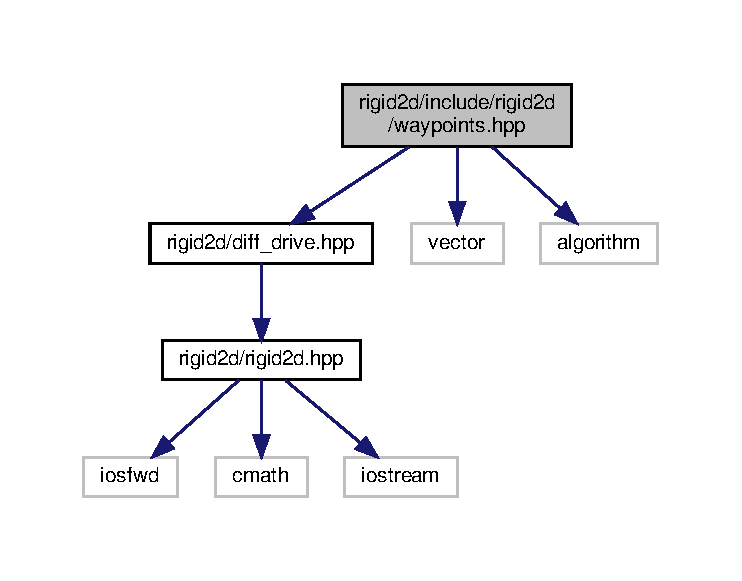
\includegraphics[width=350pt]{d1/d11/waypoints_8hpp__incl}
\end{center}
\end{figure}
This graph shows which files directly or indirectly include this file\+:\nopagebreak
\begin{figure}[H]
\begin{center}
\leavevmode
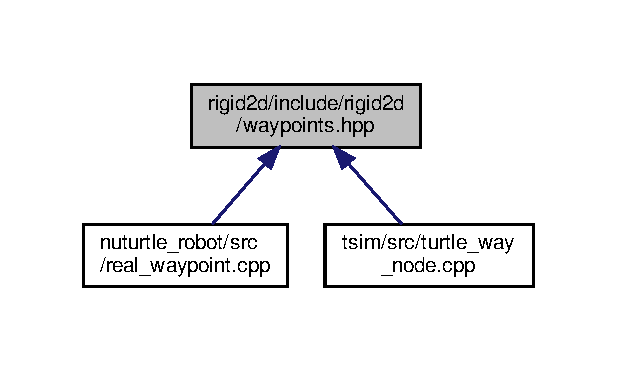
\includegraphics[width=296pt]{d0/d66/waypoints_8hpp__dep__incl}
\end{center}
\end{figure}
\subsection*{Classes}
\begin{DoxyCompactItemize}
\item 
class \hyperlink{classrigid2d_1_1Waypoints}{rigid2d\+::\+Waypoints}
\end{DoxyCompactItemize}


\subsection{Detailed Description}
Library Diff\+Drive robot kinematics and odometry. 


\hypertarget{fake__diff__encoders__node_8cpp}{}\section{rigid2d/src/fake\+\_\+diff\+\_\+encoders\+\_\+node.cpp File Reference}
\label{fake__diff__encoders__node_8cpp}\index{rigid2d/src/fake\+\_\+diff\+\_\+encoders\+\_\+node.\+cpp@{rigid2d/src/fake\+\_\+diff\+\_\+encoders\+\_\+node.\+cpp}}


Main\+: Publishes Fake Encoder Messages to /joint\+\_\+states.  


{\ttfamily \#include $<$ros/ros.\+h$>$}\newline
{\ttfamily \#include $<$geometry\+\_\+msgs/\+Twist.\+h$>$}\newline
{\ttfamily \#include $<$sensor\+\_\+msgs/\+Joint\+State.\+h$>$}\newline
{\ttfamily \#include $<$string$>$}\newline
{\ttfamily \#include \char`\"{}rigid2d/rigid2d.\+hpp\char`\"{}}\newline
{\ttfamily \#include \char`\"{}rigid2d/diff\+\_\+drive.\+hpp\char`\"{}}\newline
Include dependency graph for fake\+\_\+diff\+\_\+encoders\+\_\+node.\+cpp\+:
\nopagebreak
\begin{figure}[H]
\begin{center}
\leavevmode
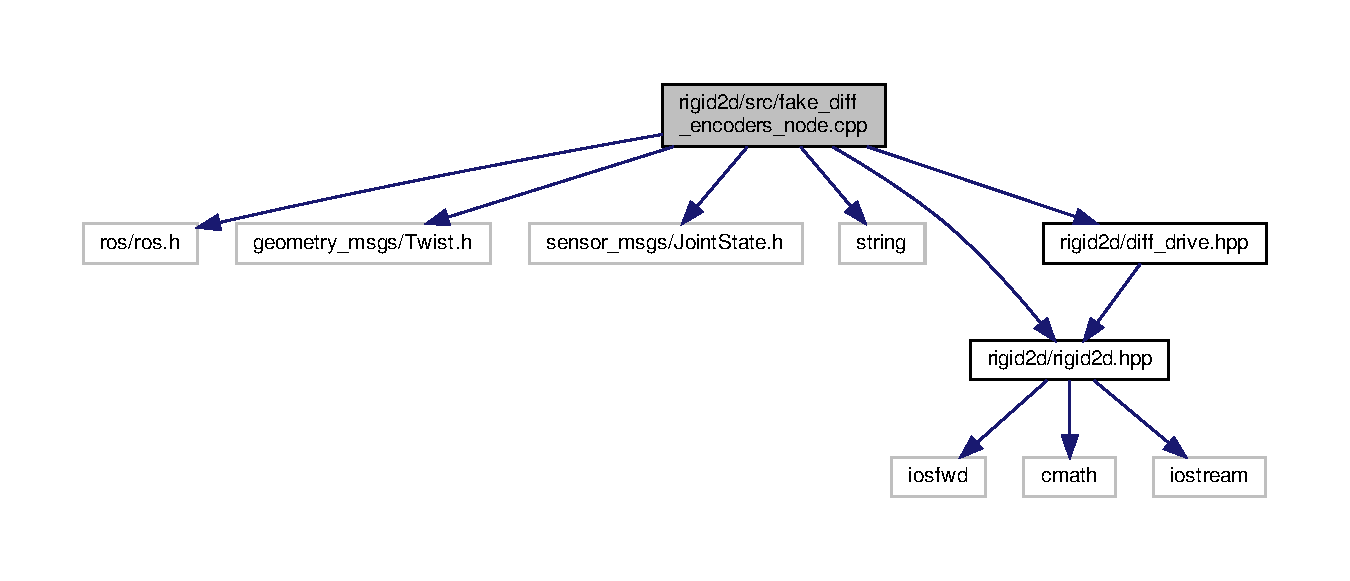
\includegraphics[width=350pt]{d4/dd2/fake__diff__encoders__node_8cpp__incl}
\end{center}
\end{figure}
\subsection*{Functions}
\begin{DoxyCompactItemize}
\item 
void \hyperlink{fake__diff__encoders__node_8cpp_a647c2d49e90958302787373cf0bf90b7}{vel\+\_\+callback} (const geometry\+\_\+msgs\+::\+Twist \&tw)
\item 
\mbox{\Hypertarget{fake__diff__encoders__node_8cpp_a3c04138a5bfe5d72780bb7e82a18e627}\label{fake__diff__encoders__node_8cpp_a3c04138a5bfe5d72780bb7e82a18e627}} 
int \hyperlink{fake__diff__encoders__node_8cpp_a3c04138a5bfe5d72780bb7e82a18e627}{main} (int argc, char $\ast$$\ast$argv)
\begin{DoxyCompactList}\small\item\em The Main Function ///. \end{DoxyCompactList}\end{DoxyCompactItemize}
\subsection*{Variables}
\begin{DoxyCompactItemize}
\item 
\mbox{\Hypertarget{fake__diff__encoders__node_8cpp_a2e231184bf093953a82dd28fe0151cd6}\label{fake__diff__encoders__node_8cpp_a2e231184bf093953a82dd28fe0151cd6}} 
\hyperlink{structrigid2d_1_1WheelVelocities}{rigid2d\+::\+Wheel\+Velocities} {\bfseries w\+\_\+ang}
\item 
\mbox{\Hypertarget{fake__diff__encoders__node_8cpp_aae05b70475acb90fabcbcb02075b4a5c}\label{fake__diff__encoders__node_8cpp_aae05b70475acb90fabcbcb02075b4a5c}} 
\hyperlink{classrigid2d_1_1DiffDrive}{rigid2d\+::\+Diff\+Drive} {\bfseries driver}
\item 
\mbox{\Hypertarget{fake__diff__encoders__node_8cpp_a4c45cdff103e6644a620ba5061509f22}\label{fake__diff__encoders__node_8cpp_a4c45cdff103e6644a620ba5061509f22}} 
double {\bfseries frequency} = 60
\item 
\mbox{\Hypertarget{fake__diff__encoders__node_8cpp_a3ee0ad2c2fb892e39c44a42e14f18ce4}\label{fake__diff__encoders__node_8cpp_a3ee0ad2c2fb892e39c44a42e14f18ce4}} 
bool {\bfseries callback\+\_\+flag} = false
\end{DoxyCompactItemize}


\subsection{Detailed Description}
Main\+: Publishes Fake Encoder Messages to /joint\+\_\+states. 

P\+A\+R\+A\+M\+E\+T\+E\+RS\+: wl\+\_\+fid\+\_\+ (string)\+: the left wheel joint name in diff\+\_\+drive.\+urdf.\+xacro of nuturtle\+\_\+desctipion pkg wr\+\_\+fid\+\_\+ (string)\+: the right wheel joint name in diff\+\_\+drive.\+urdf.\+xacro of nuturtle\+\_\+desctipion pkg wbase\+\_\+ (float)\+: wheel base of modeled diff drive robot wrad\+\_\+ (float)\+: wheel radius of modeled diff drive robot frequency (int)\+: frequency of control loop. callback\+\_\+flag (bool)\+: specifies whether to send a new transform (only when new pose is read)

pose (\hyperlink{structrigid2d_1_1Pose2D}{rigid2d\+::\+Pose2D})\+: modeled diff drive robot pose based on read wheel encoder angles wl\+\_\+enc (float)\+: left wheel encoder angles wr\+\_\+enc (float)\+: right wheel encoder angles driver (\hyperlink{classrigid2d_1_1DiffDrive}{rigid2d\+::\+Diff\+Drive})\+: model of the diff drive robot Vb (\hyperlink{classrigid2d_1_1Twist2D}{rigid2d\+::\+Twist2D})\+: read from cmd\+\_\+vel subscriber w\+\_\+ang (\hyperlink{structrigid2d_1_1WheelVelocities}{rigid2d\+::\+Wheel\+Velocities})\+: wheel angles used to calculate ddrive robot twist (overloaded struct)

js (sensor\+\_\+msgs\+::\+Joint\+State)\+: used to publish simulated wheel encoder readings to /joint\+\_\+states topic

P\+U\+B\+L\+I\+S\+H\+ES\+: js (sensor\+\_\+msgs\+::\+Joint\+State)\+: publishes joint state message containing left and right wheel angles S\+U\+B\+S\+C\+R\+I\+B\+ES\+: /cmd\+\_\+vel (geometry\+\_\+msgs\+::\+Twist)\+: subscriber, which records the commanded twist

F\+U\+N\+C\+T\+I\+O\+NS\+: vel\+\_\+callback (void)\+: callback for /cmd\+\_\+vel subscriber, which records the commanded twist 

\subsection{Function Documentation}
\mbox{\Hypertarget{fake__diff__encoders__node_8cpp_a647c2d49e90958302787373cf0bf90b7}\label{fake__diff__encoders__node_8cpp_a647c2d49e90958302787373cf0bf90b7}} 
\index{fake\+\_\+diff\+\_\+encoders\+\_\+node.\+cpp@{fake\+\_\+diff\+\_\+encoders\+\_\+node.\+cpp}!vel\+\_\+callback@{vel\+\_\+callback}}
\index{vel\+\_\+callback@{vel\+\_\+callback}!fake\+\_\+diff\+\_\+encoders\+\_\+node.\+cpp@{fake\+\_\+diff\+\_\+encoders\+\_\+node.\+cpp}}
\subsubsection{\texorpdfstring{vel\+\_\+callback()}{vel\_callback()}}
{\footnotesize\ttfamily void vel\+\_\+callback (\begin{DoxyParamCaption}\item[{const geometry\+\_\+msgs\+::\+Twist \&}]{tw }\end{DoxyParamCaption})}

cmd\+\_\+vel subscriber callback. Records commanded twist


\begin{DoxyParams}{Parameters}
{\em tw} & (geometry\+\_\+msgs\+::\+Twist)\+: the commanded linear and angular velocity \\
\hline
\end{DoxyParams}
\begin{DoxyReturn}{Returns}
w\+\_\+ang (\hyperlink{structrigid2d_1_1WheelVelocities}{rigid2d\+::\+Wheel\+Velocities})\+: the left and right wheel angles
\end{DoxyReturn}
This function runs every time we get a geometry\+\_\+msgs\+::\+Twist message on the \char`\"{}cmd\+\_\+vel\char`\"{} topic. We generally use the const $<$message$>$Const\+Ptr \&msg syntax to prevent our node from accidentally changing the message, in the case that another node is also listening to it.
\hypertarget{odometer__node_8cpp}{}\section{rigid2d/src/odometer\+\_\+node.cpp File Reference}
\label{odometer__node_8cpp}\index{rigid2d/src/odometer\+\_\+node.\+cpp@{rigid2d/src/odometer\+\_\+node.\+cpp}}


Main\+: Publishes Odometry messages for diff drive robot based on wheel joint states.  


{\ttfamily \#include $<$ros/ros.\+h$>$}\newline
{\ttfamily \#include $<$sensor\+\_\+msgs/\+Joint\+State.\+h$>$}\newline
{\ttfamily \#include $<$nav\+\_\+msgs/\+Odometry.\+h$>$}\newline
{\ttfamily \#include $<$tf2/\+Linear\+Math/\+Quaternion.\+h$>$}\newline
{\ttfamily \#include $<$tf2\+\_\+ros/transform\+\_\+broadcaster.\+h$>$}\newline
{\ttfamily \#include $<$tf2\+\_\+geometry\+\_\+msgs/tf2\+\_\+geometry\+\_\+msgs.\+h$>$}\newline
{\ttfamily \#include \char`\"{}rigid2d/\+Set\+Pose.\+h\char`\"{}}\newline
{\ttfamily \#include $<$string$>$}\newline
{\ttfamily \#include \char`\"{}rigid2d/rigid2d.\+hpp\char`\"{}}\newline
{\ttfamily \#include \char`\"{}rigid2d/diff\+\_\+drive.\+hpp\char`\"{}}\newline
Include dependency graph for odometer\+\_\+node.\+cpp\+:\nopagebreak
\begin{figure}[H]
\begin{center}
\leavevmode
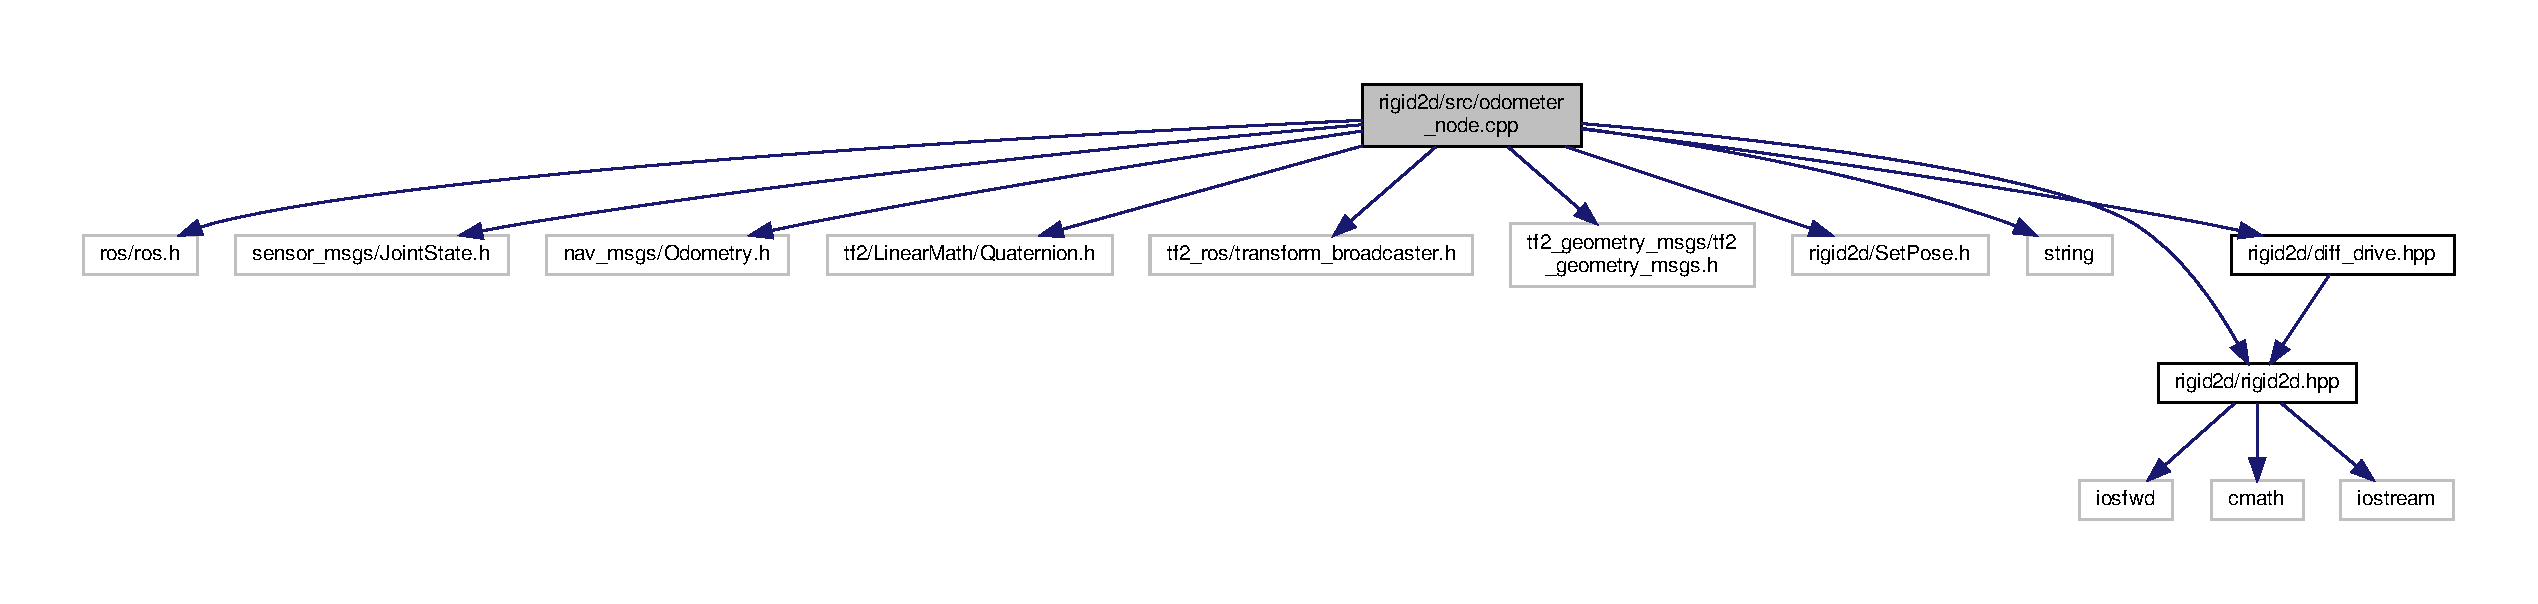
\includegraphics[width=350pt]{d9/d43/odometer__node_8cpp__incl}
\end{center}
\end{figure}
\subsection*{Functions}
\begin{DoxyCompactItemize}
\item 
void \hyperlink{odometer__node_8cpp_a8f0c3d2ac4fed55d807bd69afb5243b4}{js\+\_\+callback} (const sensor\+\_\+msgs\+::\+Joint\+State\+::\+Const\+Ptr \&js)
\item 
bool \hyperlink{odometer__node_8cpp_adb6929707bcc4d4fb332481cb33e4f2b}{set\+\_\+pose\+Callback} (rigid2d\+::\+Set\+Pose\+::\+Request \&req, rigid2d\+::\+Set\+Pose\+::\+Response \&res)
\begin{DoxyCompactList}\small\item\em set\+\_\+pose service callback. Sets the turtlebot\textquotesingle{}s pose belief to desired value. \end{DoxyCompactList}\item 
\mbox{\Hypertarget{odometer__node_8cpp_a3c04138a5bfe5d72780bb7e82a18e627}\label{odometer__node_8cpp_a3c04138a5bfe5d72780bb7e82a18e627}} 
int \hyperlink{odometer__node_8cpp_a3c04138a5bfe5d72780bb7e82a18e627}{main} (int argc, char $\ast$$\ast$argv)
\begin{DoxyCompactList}\small\item\em The Main Function ///. \end{DoxyCompactList}\end{DoxyCompactItemize}
\subsection*{Variables}
\begin{DoxyCompactItemize}
\item 
\mbox{\Hypertarget{odometer__node_8cpp_ad1ee493a9c3d90ec79d68e9de39a0d62}\label{odometer__node_8cpp_ad1ee493a9c3d90ec79d68e9de39a0d62}} 
float {\bfseries wl\+\_\+enc} = 0
\item 
\mbox{\Hypertarget{odometer__node_8cpp_a82d2473bdd4614b5a4532a95a0382487}\label{odometer__node_8cpp_a82d2473bdd4614b5a4532a95a0382487}} 
float {\bfseries wr\+\_\+enc} = 0
\item 
\mbox{\Hypertarget{odometer__node_8cpp_abb35a308e88b2a5d113795948e6273a3}\label{odometer__node_8cpp_abb35a308e88b2a5d113795948e6273a3}} 
\hyperlink{classrigid2d_1_1Twist2D}{rigid2d\+::\+Twist2D} {\bfseries Vb}
\item 
\mbox{\Hypertarget{odometer__node_8cpp_a002f817728ce76d60fecd0d2b5bcd214}\label{odometer__node_8cpp_a002f817728ce76d60fecd0d2b5bcd214}} 
\hyperlink{structrigid2d_1_1WheelVelocities}{rigid2d\+::\+Wheel\+Velocities} {\bfseries w\+\_\+vel}
\item 
\mbox{\Hypertarget{odometer__node_8cpp_aabf3dfeb602efbe1bc76a7918ae6e838}\label{odometer__node_8cpp_aabf3dfeb602efbe1bc76a7918ae6e838}} 
\hyperlink{structrigid2d_1_1Pose2D}{rigid2d\+::\+Pose2D} {\bfseries reset\+\_\+pose}
\item 
\mbox{\Hypertarget{odometer__node_8cpp_aae05b70475acb90fabcbcb02075b4a5c}\label{odometer__node_8cpp_aae05b70475acb90fabcbcb02075b4a5c}} 
\hyperlink{classrigid2d_1_1DiffDrive}{rigid2d\+::\+Diff\+Drive} {\bfseries driver}
\item 
\mbox{\Hypertarget{odometer__node_8cpp_a3ee0ad2c2fb892e39c44a42e14f18ce4}\label{odometer__node_8cpp_a3ee0ad2c2fb892e39c44a42e14f18ce4}} 
bool {\bfseries callback\+\_\+flag} = true
\item 
\mbox{\Hypertarget{odometer__node_8cpp_a13c6e8170f4eaffabda3cd95e02d139c}\label{odometer__node_8cpp_a13c6e8170f4eaffabda3cd95e02d139c}} 
bool {\bfseries service\+\_\+flag} = false
\end{DoxyCompactItemize}


\subsection{Detailed Description}
Main\+: Publishes Odometry messages for diff drive robot based on wheel joint states. 

P\+A\+R\+A\+M\+E\+T\+E\+RS\+: o\+\_\+fid\+\_\+ (string)\+: parent frame ID for the published tf transform o\+\_\+fid\+\_\+ (string)\+: child frame ID for the published tf transform wbase\+\_\+ (float)\+: wheel base of modeled diff drive robot wrad\+\_\+ (float)\+: wheel radius of modeled diff drive robot frequency (int)\+: frequency of control loop. callback\+\_\+flag (bool)\+: specifies whether to send a new transform (only when new pose is read)

pose (\hyperlink{structrigid2d_1_1Pose2D}{rigid2d\+::\+Pose2D})\+: modeled diff drive robot pose based on read wheel encoder angles wl\+\_\+enc (float)\+: left wheel encoder angles wr\+\_\+enc (float)\+: right wheel encoder angles driver (\hyperlink{classrigid2d_1_1DiffDrive}{rigid2d\+::\+Diff\+Drive})\+: model of the diff drive robot Vb (\hyperlink{classrigid2d_1_1Twist2D}{rigid2d\+::\+Twist2D})\+: read from driver instances to publish to odom message w\+\_\+vel (\hyperlink{structrigid2d_1_1WheelVelocities}{rigid2d\+::\+Wheel\+Velocities})\+: wheel velocities used to calculate ddrive robot twist

odom\+\_\+tf (geometry\+\_\+msgs\+::\+Transform\+Stamped)\+: odometry frame transform used to update R\+Viz sim odom (nav\+\_\+msgs\+::\+Odometry)\+: odometry message containing pose and twist published to odom topic

P\+U\+B\+L\+I\+S\+H\+ES\+: odom (nav\+\_\+msgs\+::\+Odometry)\+: publishes odometry message containing pose(x,y,z) and twist(lin,ang) S\+U\+B\+S\+C\+R\+I\+B\+ES\+: /joint\+\_\+states (sensor\+\_\+msgs\+::\+Joint\+State), which records the ddrive robot\textquotesingle{}s joint states

F\+U\+N\+C\+T\+I\+O\+NS\+: js\+\_\+callback (void)\+: callback for /joint\+\_\+states subscriber, which records the ddrive robot\textquotesingle{}s joint states set\+\_\+pose\+Callback (bool)\+: callback for set\+\_\+pose service, which resets the robot\textquotesingle{}s pose in the tf tree 

\subsection{Function Documentation}
\mbox{\Hypertarget{odometer__node_8cpp_a8f0c3d2ac4fed55d807bd69afb5243b4}\label{odometer__node_8cpp_a8f0c3d2ac4fed55d807bd69afb5243b4}} 
\index{odometer\+\_\+node.\+cpp@{odometer\+\_\+node.\+cpp}!js\+\_\+callback@{js\+\_\+callback}}
\index{js\+\_\+callback@{js\+\_\+callback}!odometer\+\_\+node.\+cpp@{odometer\+\_\+node.\+cpp}}
\subsubsection{\texorpdfstring{js\+\_\+callback()}{js\_callback()}}
{\footnotesize\ttfamily void js\+\_\+callback (\begin{DoxyParamCaption}\item[{const sensor\+\_\+msgs\+::\+Joint\+State\+::\+Const\+Ptr \&}]{js }\end{DoxyParamCaption})}

/joint\+\_\+states subscriber callback. Records left and right wheel angles


\begin{DoxyParams}{Parameters}
{\em js} & (sensor\+\_\+msgs\+::\+Joint\+State)\+: the left and right wheel joint angles \\
\hline
\end{DoxyParams}
\begin{DoxyReturn}{Returns}
pose (\hyperlink{structrigid2d_1_1Pose2D}{rigid2d\+::\+Pose2D})\+: modeled diff drive robot pose based on read wheel encoder angles
\end{DoxyReturn}
This function runs every time we get a sensor\+\_\+msgs\+::\+Joint\+State message on the \char`\"{}/joint\+\_\+states\char`\"{} topic. We generally use the const $<$message$>$Const\+Ptr \&msg syntax to prevent our node from accidentally changing the message, in the case that another node is also listening to it.\mbox{\Hypertarget{odometer__node_8cpp_adb6929707bcc4d4fb332481cb33e4f2b}\label{odometer__node_8cpp_adb6929707bcc4d4fb332481cb33e4f2b}} 
\index{odometer\+\_\+node.\+cpp@{odometer\+\_\+node.\+cpp}!set\+\_\+pose\+Callback@{set\+\_\+pose\+Callback}}
\index{set\+\_\+pose\+Callback@{set\+\_\+pose\+Callback}!odometer\+\_\+node.\+cpp@{odometer\+\_\+node.\+cpp}}
\subsubsection{\texorpdfstring{set\+\_\+pose\+Callback()}{set\_poseCallback()}}
{\footnotesize\ttfamily bool set\+\_\+pose\+Callback (\begin{DoxyParamCaption}\item[{rigid2d\+::\+Set\+Pose\+::\+Request \&}]{req,  }\item[{rigid2d\+::\+Set\+Pose\+::\+Response \&}]{res }\end{DoxyParamCaption})}



set\+\_\+pose service callback. Sets the turtlebot\textquotesingle{}s pose belief to desired value. 


\begin{DoxyParams}{Parameters}
{\em x} & (float32)\+: desired x pose. \\
\hline
{\em y} & (float32)\+: desired y pose. \\
\hline
{\em theta} & (float32)\+: desired theta pose. \\
\hline
\end{DoxyParams}
\begin{DoxyReturn}{Returns}
result (bool)\+: True or False. 
\end{DoxyReturn}

\hypertarget{turtle__rect_8cpp}{}\section{tsim/src/turtle\+\_\+rect.cpp File Reference}
\label{turtle__rect_8cpp}\index{tsim/src/turtle\+\_\+rect.\+cpp@{tsim/src/turtle\+\_\+rect.\+cpp}}


Class Constructor for Turtle\+Rect.  


{\ttfamily \#include \char`\"{}tsim/turtle\+\_\+rect.\+h\char`\"{}}\newline
Include dependency graph for turtle\+\_\+rect.\+cpp\+:
\nopagebreak
\begin{figure}[H]
\begin{center}
\leavevmode
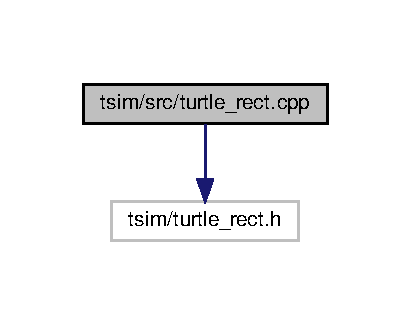
\includegraphics[width=197pt]{d7/df1/turtle__rect_8cpp__incl}
\end{center}
\end{figure}


\subsection{Detailed Description}
Class Constructor for Turtle\+Rect. 

P\+A\+R\+A\+M\+E\+T\+E\+RS\+: x\+\_\+ (int)\+: x coordinate for lower left corner of rectangle. y\+\_\+ (int)\+: y coordinate for lower left corner of rectangle. width\+\_\+ (int)\+: width of rectangle. height\+\_\+ (int)\+: height of rectangle. trans\+\_\+vel\+\_\+ (int)\+: translational velocity of robot. rot\+\_\+vel\+\_\+ (int)\+: rotational velocity of robot. frequency\+\_\+ (int)\+: frequency of control loop. threshold\+\_\+ (float)\+: specifies when the target pose has been reached.

goal\+\_\+x (float)\+: target turtle position in x. goal\+\_\+y (float)\+: target turtle position in y. goal\+\_\+head (float)\+: target turtle position in theta.

x\+\_\+pos\+\_\+ (float)\+: turtle position in x read from turtle1/pose topic. y\+\_\+pos\+\_\+ (float)\+: turtle position in y read from turtle1/pose topic. head\+\_\+ (float)\+: turtle position in theta read from turtle1/pose topic.

x\+\_\+o\+\_\+ (float)\+: turtle position in x predicted using forward model propagation. y\+\_\+o\+\_\+ (float)\+: turtle position in y predicted using forward model propagation. head\+\_\+o\+\_\+ (float)\+: turtle position in theta predicted using forward model propagation.

x\+\_\+error\+\_\+ (float)\+: turtle position error in x between read and predicted values. y\+\_\+error\+\_\+ (float)\+: turtle position error in y between read and predicted values. theta\+\_\+error\+\_\+ (float)\+: turtle position error in theta between read and predicted values.

pose\+\_\+error\+\_\+ (Pose\+Error)\+: custom message that stores x\+\_\+error, y\+\_\+error and theta\+\_\+error. twist\+\_\+ (Twist)\+: used to publish linear and angular velocities to turtle1/cmd\+\_\+vel.

done\+\_\+flag\+\_\+ (bool)\+: true when correct position or heading has been achieved in loop. lin\+\_\+ang\+\_\+flag\+\_\+ (bool)\+: true when angular velocity should be applied, linear otherwise. count)vertex\+\_\+ (int)\+: counter which resets to zero once all rectangle vertices have been reached.

F\+U\+N\+C\+T\+I\+O\+NS\+: traj\+\_\+reset\+Callback (bool)\+: callback for traj\+\_\+reset service, which teleports turtle back to initial config. pose\+Callback (void)\+: callback for turtle1/pose subscriber, which records the turtle\textquotesingle{}s pose for use elsewhere. move (void)\+: helper function which publishes Twist messages to turtle1/cmd\+\_\+vel to actuate the turtle. predict(void)\+: helper function which forward propagates the open-\/loop model and publishes Pose\+Error to pose\+\_\+error. control(void)\+: main class method. Houses state machine and calls helper function to perform trajectory and plot.

taken from \href{https://magiccvs.byu.edu/wiki/#!ros_tutorials/c++_node_class.md}{\tt https\+://magiccvs.\+byu.\+edu/wiki/\#!ros\+\_\+tutorials/c++\+\_\+node\+\_\+class.\+md} 
\hypertarget{turtle__rect__node_8cpp}{}\section{tsim/src/turtle\+\_\+rect\+\_\+node.cpp File Reference}
\label{turtle__rect__node_8cpp}\index{tsim/src/turtle\+\_\+rect\+\_\+node.\+cpp@{tsim/src/turtle\+\_\+rect\+\_\+node.\+cpp}}


Main\+: makes turtle in turtlesim move in a rectangular trajectory.  


{\ttfamily \#include $<$ros/ros.\+h$>$}\newline
{\ttfamily \#include $<$turtlesim/\+Pose.\+h$>$}\newline
{\ttfamily \#include $<$geometry\+\_\+msgs/\+Twist.\+h$>$}\newline
{\ttfamily \#include $<$std\+\_\+srvs/\+Empty.\+h$>$}\newline
{\ttfamily \#include \char`\"{}tsim/turtle\+\_\+rect.\+h\char`\"{}}\newline
Include dependency graph for turtle\+\_\+rect\+\_\+node.\+cpp\+:\nopagebreak
\begin{figure}[H]
\begin{center}
\leavevmode
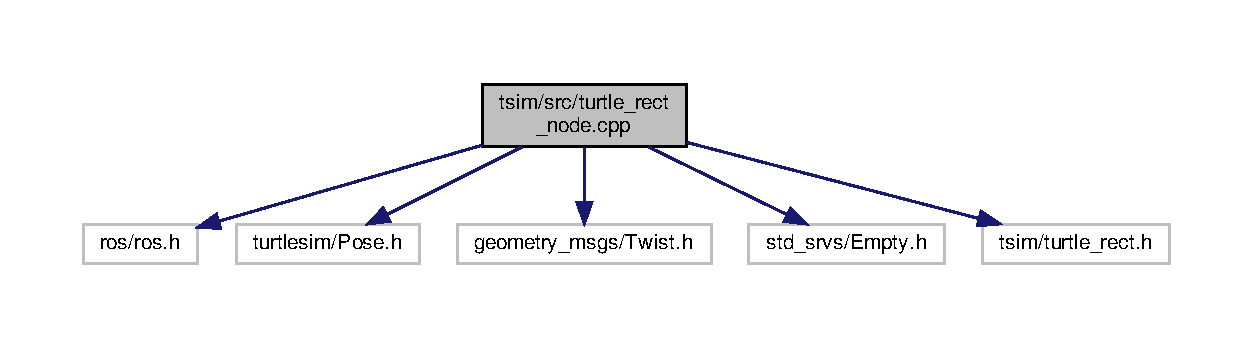
\includegraphics[width=350pt]{d5/d1c/turtle__rect__node_8cpp__incl}
\end{center}
\end{figure}
\subsection*{Functions}
\begin{DoxyCompactItemize}
\item 
\mbox{\Hypertarget{turtle__rect__node_8cpp_a3c04138a5bfe5d72780bb7e82a18e627}\label{turtle__rect__node_8cpp_a3c04138a5bfe5d72780bb7e82a18e627}} 
int \hyperlink{turtle__rect__node_8cpp_a3c04138a5bfe5d72780bb7e82a18e627}{main} (int argc, char $\ast$$\ast$argv)
\begin{DoxyCompactList}\small\item\em The Main Function ///. \end{DoxyCompactList}\end{DoxyCompactItemize}


\subsection{Detailed Description}
Main\+: makes turtle in turtlesim move in a rectangular trajectory. 

P\+A\+R\+A\+M\+E\+T\+E\+RS\+: x (int)\+: x coordinate for lower left corner of rectangle. y (int)\+: y coordinate for lower left corner of rectangle. width (int)\+: width of rectangle. height (int)\+: height of rectangle. trans\+\_\+vel (int)\+: translational velocity of robot. rot\+\_\+vel (int)\+: rotational velocity of robot. frequency(int)\+: frequency of control loop. threshold(float)\+: specifies when the target pose has been reached. P\+U\+B\+L\+I\+S\+H\+ES\+: turtle1/cmd\+\_\+vel (Twist)\+: publishes a twist with linear (x) and angular (z) velocities to command turtle pose\+\_\+error (Pose\+Error)\+: publishes pose error in x, y, and theta for plotting S\+U\+B\+S\+C\+R\+I\+B\+ES\+: turtle1/pose (Pose)\+: feceives the x, y, and theta position of the turtle from turtlesim. S\+E\+R\+V\+I\+C\+ES\+: traj\+\_\+reset (Empty)\+: teleports the turtle back to (x,y) with 0 heading, and without leaving a pen trace. also resets the predicted pose estimate to these values.

taken from \href{https://magiccvs.byu.edu/wiki/#!ros_tutorials/c++_node_class.md}{\tt https\+://magiccvs.\+byu.\+edu/wiki/\#!ros\+\_\+tutorials/c++\+\_\+node\+\_\+class.\+md} 
\hypertarget{turtle__way__node_8cpp}{}\section{tsim/src/turtle\+\_\+way\+\_\+node.cpp File Reference}
\label{turtle__way__node_8cpp}\index{tsim/src/turtle\+\_\+way\+\_\+node.\+cpp@{tsim/src/turtle\+\_\+way\+\_\+node.\+cpp}}


Makes turtlesim modeled as Diff Drive robot follow a user-\/specified trajectory in turtle\+\_\+way.\+yaml.  


{\ttfamily \#include $<$ros/ros.\+h$>$}\newline
{\ttfamily \#include $<$turtlesim/\+Pose.\+h$>$}\newline
{\ttfamily \#include $<$geometry\+\_\+msgs/\+Twist.\+h$>$}\newline
{\ttfamily \#include $<$std\+\_\+srvs/\+Empty.\+h$>$}\newline
{\ttfamily \#include $<$tsim/\+Pose\+Error.\+h$>$}\newline
{\ttfamily \#include $<$turtlesim/\+Set\+Pen.\+h$>$}\newline
{\ttfamily \#include $<$turtlesim/\+Teleport\+Absolute.\+h$>$}\newline
{\ttfamily \#include $<$math.\+h$>$}\newline
{\ttfamily \#include $<$string$>$}\newline
{\ttfamily \#include $<$vector$>$}\newline
{\ttfamily \#include $<$boost/iterator/zip\+\_\+iterator.\+hpp$>$}\newline
{\ttfamily \#include \char`\"{}rigid2d/waypoints.\+hpp\char`\"{}}\newline
Include dependency graph for turtle\+\_\+way\+\_\+node.\+cpp\+:\nopagebreak
\begin{figure}[H]
\begin{center}
\leavevmode
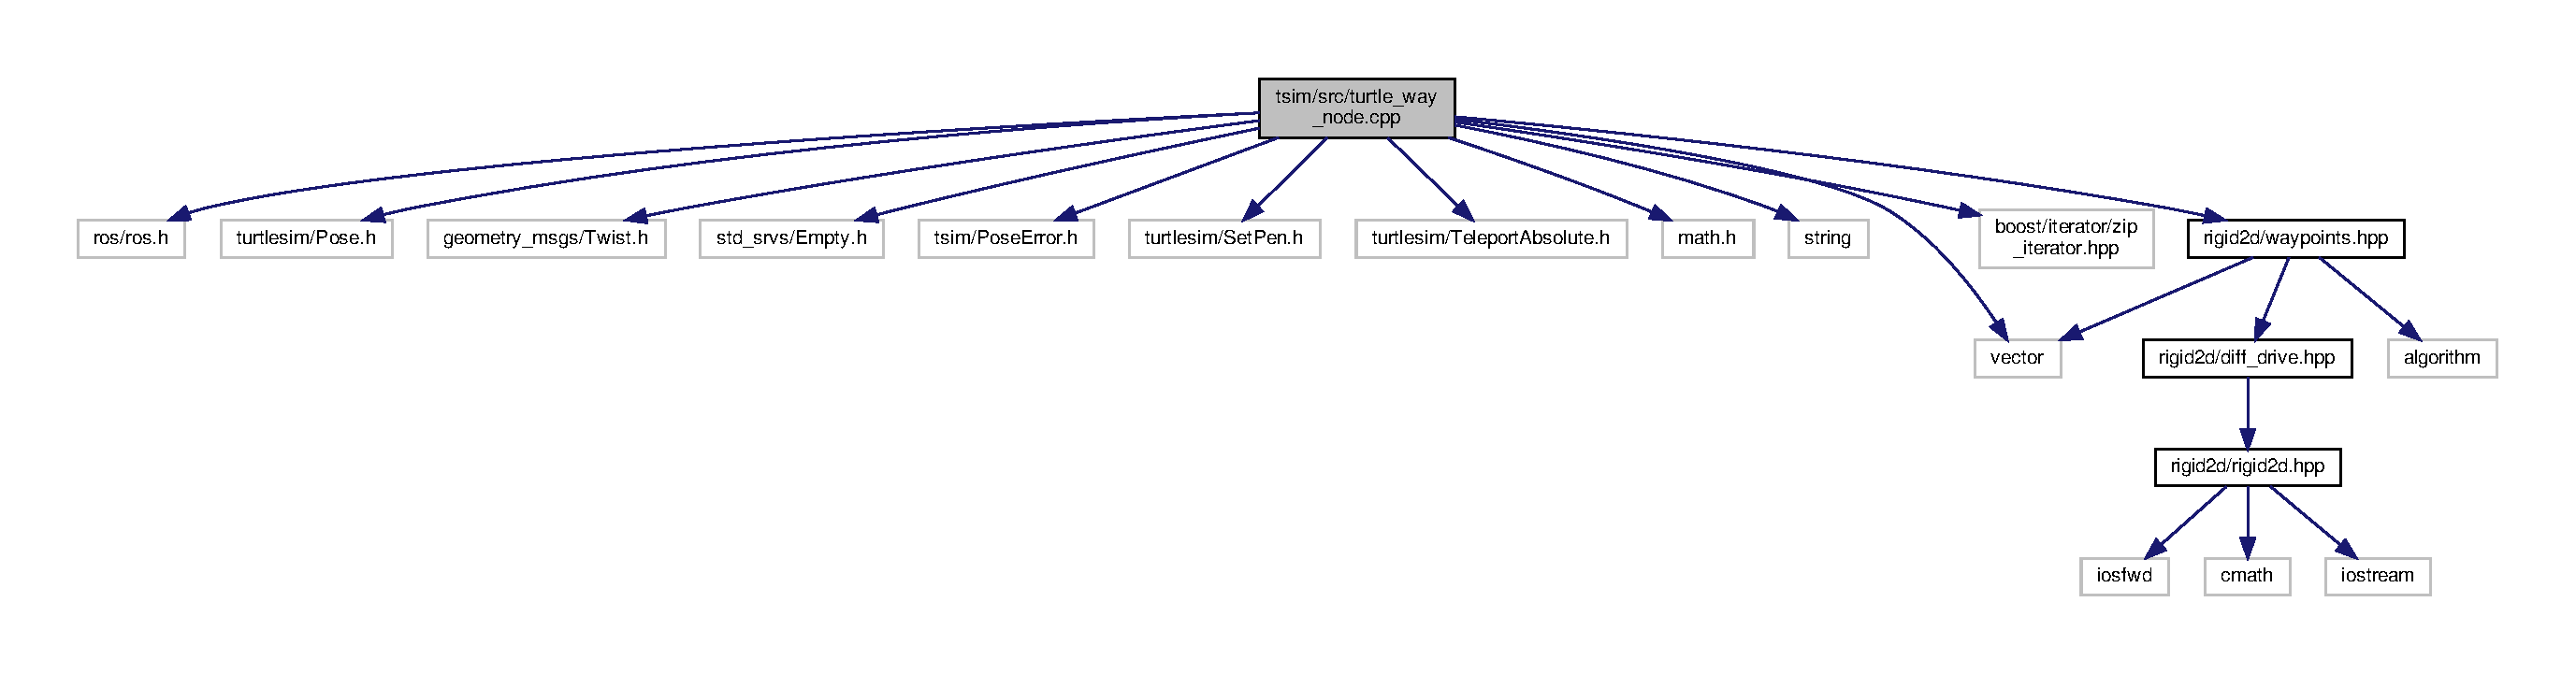
\includegraphics[width=350pt]{d2/d39/turtle__way__node_8cpp__incl}
\end{center}
\end{figure}
\subsection*{Functions}
\begin{DoxyCompactItemize}
\item 
void \hyperlink{turtle__way__node_8cpp_a32f38e8ed5c6dc1fe5766d378c21f115}{pose\+Callback} (const turtlesim\+::\+Pose\+Const\+Ptr \&pos)
\item 
\mbox{\Hypertarget{turtle__way__node_8cpp_a3c04138a5bfe5d72780bb7e82a18e627}\label{turtle__way__node_8cpp_a3c04138a5bfe5d72780bb7e82a18e627}} 
int \hyperlink{turtle__way__node_8cpp_a3c04138a5bfe5d72780bb7e82a18e627}{main} (int argc, char $\ast$$\ast$argv)
\begin{DoxyCompactList}\small\item\em The Main Function ///. \end{DoxyCompactList}\end{DoxyCompactItemize}
\subsection*{Variables}
\begin{DoxyCompactItemize}
\item 
\mbox{\Hypertarget{turtle__way__node_8cpp_aff33052d2147e2cb1ed2cfbc439023df}\label{turtle__way__node_8cpp_aff33052d2147e2cb1ed2cfbc439023df}} 
\hyperlink{structrigid2d_1_1Pose2D}{Pose2D} {\bfseries pose}
\end{DoxyCompactItemize}


\subsection{Detailed Description}
Makes turtlesim modeled as Diff Drive robot follow a user-\/specified trajectory in turtle\+\_\+way.\+yaml. 

P\+A\+R\+A\+M\+E\+T\+E\+RS\+: waypoint\+\_\+x (vector$<$float$>$)\+: x-\/coordinates of the waypoints to visit waypoint\+\_\+y (vector$<$float$>$)\+: y-\/coordinates of the waypoints to visit frequency (int)\+: frequency of control loop. threshold (float)\+: specifies when the target pose has been reached.

pose (turtlesim\+::\+Pose)\+: turtle position as read by turtle1/pose topic driver\+\_\+pose (\hyperlink{structrigid2d_1_1Pose2D}{rigid2d\+::\+Pose2D})\+: modeled diff drive robot pose based on feedforward prediction

x\+\_\+error (float)\+: turtle position error in x between read and predicted values. y\+\_\+error (float)\+: turtle position error in y between read and predicted values. theta\+\_\+error (float)\+: turtle position error in theta between read and predicted values. pose\+\_\+error (Pose\+Error)\+: custom message that stores x\+\_\+error, y\+\_\+error and theta\+\_\+error. tw (Twist)\+: used to publish linear and angular velocities to turtle1/cmd\+\_\+vel.

Vb (\hyperlink{classrigid2d_1_1Twist2D}{rigid2d\+::\+Twist2D})\+: scaled from tw based on loop rate to predict simulated diff drive robot path driver (\hyperlink{classrigid2d_1_1DiffDrive}{rigid2d\+::\+Diff\+Drive})\+: model of the diff drive robot waypoints\+\_\+ (vector$<$rigid2d\+::\+Vector2\+D$>$)\+: intermediate storage of waypoints combined using waypoint\+\_\+x and y waypoints (\hyperlink{classrigid2d_1_1Waypoints}{rigid2d\+::\+Waypoints})\+: stores waypoints to visit and returns \hyperlink{classrigid2d_1_1Twist2D}{rigid2d\+::\+Twist2D} required to do so

P\+U\+B\+L\+I\+S\+H\+ES\+: turtle1/cmd\+\_\+vel (geometry\+\_\+msgs\+::\+Twist)\+: publishes a twist with linear (x) and angular (z) velocities to command turtle pose\+\_\+error (tsim\+:Pose\+Error)\+: publishes pose error in x, y, and theta for plotting S\+U\+B\+S\+C\+R\+I\+B\+ES\+: turtle1/pose (turtlesim\+::\+Pose)\+: feceives the x, y, and theta position of the turtle from turtlesim.

F\+U\+N\+C\+T\+I\+O\+NS\+: pose\+Callback (void)\+: callback for turtle1/pose subscriber, which records the turtle\textquotesingle{}s pose for use elsewhere. 

\subsection{Function Documentation}
\mbox{\Hypertarget{turtle__way__node_8cpp_a32f38e8ed5c6dc1fe5766d378c21f115}\label{turtle__way__node_8cpp_a32f38e8ed5c6dc1fe5766d378c21f115}} 
\index{turtle\+\_\+way\+\_\+node.\+cpp@{turtle\+\_\+way\+\_\+node.\+cpp}!pose\+Callback@{pose\+Callback}}
\index{pose\+Callback@{pose\+Callback}!turtle\+\_\+way\+\_\+node.\+cpp@{turtle\+\_\+way\+\_\+node.\+cpp}}
\subsubsection{\texorpdfstring{pose\+Callback()}{poseCallback()}}
{\footnotesize\ttfamily void pose\+Callback (\begin{DoxyParamCaption}\item[{const turtlesim\+::\+Pose\+Const\+Ptr \&}]{pos }\end{DoxyParamCaption})}

turtle1/pose subscriber callback. Records turtle1 pose (x, y, theta)


\begin{DoxyParams}{Parameters}
{\em pos} & (turtlesim\+::\+Pose)\+: turtle1\textquotesingle{}s pose in x, y, and theta. \\
\hline
\end{DoxyParams}
\begin{DoxyReturn}{Returns}
pose (turtlesim\+::\+Pose)
\end{DoxyReturn}
This function runs every time we get a turtlesim\+::\+Pose message on the \char`\"{}turtle1/pose\char`\"{} topic. We generally use the const $<$message$>$Const\+Ptr \&msg syntax to prevent our node from accidentally changing the message, in the case that another node is also listening to it.
%--- End generated contents ---

% Index
\backmatter
\newpage
\phantomsection
\clearemptydoublepage
\addcontentsline{toc}{chapter}{Index}
\printindex

\end{document}
